% ------------------------------------------------------------------
% Submitted manuscript -- IEEE Transactions on Control Systems Technology (Paper)
% IEEEtran journal, two columns. All figures are pgfplots/TikZ (figures/*.tex) with data in figures/data/*.csv.
% Submitted November 2026 (PaperPlaza no. 26-1618); the release tag v0.8.0 reproduces the results.
% Compile: pdflatex three times (inline bibliography).
% ------------------------------------------------------------------
\pdfminorversion=4
\documentclass[journal]{IEEEtran}
\usepackage{amsmath,amssymb,bm}
\usepackage{booktabs}
\usepackage{siunitx}
\usepackage{graphicx}
\usepackage{cite}
\usepackage{xcolor}
\usepackage{pgfplots}
% Common pgfplots style for the manuscript figures (v0.8).
% Okabe--Ito palette; every series also differs in line style or marker (readable in greyscale).
\usepgfplotslibrary{groupplots,fillbetween}
\usetikzlibrary{plotmarks,patterns,calc,arrows.meta,positioning,decorations.pathreplacing}
\pgfplotsset{compat=1.18}
\definecolor{cRef}{HTML}{000000}
\definecolor{cGB}{HTML}{D55E00}    % grey-box EKF (vermilion)
\definecolor{cSPMe}{HTML}{56B4E9}  % SPMe UKF (sky blue)
\definecolor{cOra}{HTML}{E69F00}
\definecolor{cGre}{HTML}{009E73}
\definecolor{cBlu}{HTML}{0072B2}
\definecolor{cPur}{HTML}{CC79A7}
\definecolor{cGrey}{HTML}{999999}
\pgfplotsset{
  paper/.style={
    font=\footnotesize,
    scale only axis,
    axis line style={line width=0.4pt},
    tick style={line width=0.4pt, black},
    major tick length=2pt, minor tick length=1.2pt,
    tick align=inside,
    every tick label/.append style={font=\footnotesize},
    label style={font=\footnotesize},
    legend style={font=\footnotesize, draw=none, fill=white, fill opacity=0.85, text opacity=1,
      inner sep=1pt, row sep=-1pt, cells={anchor=west}},
    legend cell align=left,
    /pgf/number format/1000 sep={},
    enlargelimits=false,
    clip mode=individual,
    ylabel shift=-2pt, xlabel shift=-2pt,
  },
  lref/.style={cRef, line width=0.8pt},
  lgb/.style={cGB, line width=0.8pt, dash pattern=on 3pt off 1.5pt},
  lspme/.style={cSPMe, line width=1.1pt, dash pattern=on 0.9pt off 1.3pt},
  panel/.style={
    every axis title/.style={at={(0,1)}, anchor=south west, xshift=-1.8em, yshift=0pt, font=\footnotesize},
  },
}
\newcommand{\ptag}[1]{\node[anchor=north east, font=\footnotesize, inner sep=2pt] at (rel axis cs:1,1) {#1};}
% panel letter at the top-left corner of the named axis' outer box
\newcommand{\plab}[2]{\node[anchor=south west, font=\footnotesize, inner sep=0pt] at ($(#1.outer north west |- #1.north)+(0,1.2mm)$) {(#2)};}
\tikzset{zero/.style={cGrey, line width=0.3pt}, vmark/.style={cGrey, line width=0.3pt}}
\pgfplotsset{barleg/.style={legend image code/.code={\fill[##1] (0cm,-0.07cm) rectangle (0.22cm,0.11cm);}},
  lineleg/.style={legend image code/.code={\draw[##1] (0cm,0cm) -- (0.45cm,0cm);}}}

\usepackage[hidelinks]{hyperref}
\sisetup{group-separator={},detect-all}

\newcommand{\vz}{\bm{z}}\newcommand{\vj}{\bm{j}}\newcommand{\vy}{\bm{y}}\newcommand{\vw}{\bm{w}}
\newcommand{\vth}{\bm{\theta}}\newcommand{\vF}{\bm{F}}\newcommand{\mA}{\bm{A}}\newcommand{\mB}{\bm{B}}
\newcommand{\mC}{\bm{C}}\newcommand{\mP}{\bm{P}}\newcommand{\mLam}{\bm{\Lambda}}\newcommand{\dd}{\mathrm{d}}
\newcommand{\ce}{c_{\mathrm{e}}}\newcommand{\Ds}{D_{\mathrm{s}}}\newcommand{\Rf}{R_{\mathrm{f}}}
\newcommand{\LAM}{\mathrm{LAM}}\newcommand{\LLI}{\mathrm{LLI}}\newcommand{\phipl}{\phi_{\mathrm{pl}}}
\newcommand{\norm}[1]{\left\lVert #1 \right\rVert}
\newcommand{\todo}[1]{\textcolor{red!70!black}{[#1]}}

\renewcommand{\dbltopfraction}{0.85}\setcounter{dbltopnumber}{3}
\begin{document}

\title{Extended Kalman Filtering on the Full Doyle--Fuller--Newman Model via the Implicit Function Theorem: Plating-Potential Estimation and Ageing Tracking}

\author{Lorenzo~Brancato, Alexander~Gabriel~Harej, Marco~Giglio, and Francesco~Cadini\thanks{This work received no external funding.}\thanks{L. Brancato, A. G. Harej, M. Giglio and F. Cadini are with the Department of Mechanical Engineering, Politecnico di Milano, Via La Masa 1, 20156 Milan, Italy (corresponding author: F. Cadini, e-mail: francesco.cadini@polimi.it).}}

\markboth{IEEE Transactions on Control Systems Technology}{Brancato \emph{et al.}: Extended Kalman filtering on the full DFN model}

\maketitle

\begin{abstract}A battery management system must charge lithium-ion cells fast without plating lithium and know how far each cell has aged, yet it measures only current, voltage and temperature. Full-order electrochemical models describe the internal potentials that decide plating, but are rarely used online: an extended Kalman filter needs the derivative of every model step, and the model hides an iterative solver. We split the Doyle--Fuller--Newman model into a linear part (diffusion), integrated exactly, and a small nonlinear part (reaction kinetics), solved by Newton's method. The implicit function theorem then gives the exact step derivative almost for free. The 653-state filter takes 7.9 ms per step, 36 times less than an unscented filter on the same model. Against a high-resolution reference, it tracks the plating potential at the separator within 0.6 mV during 2C charge pulses, where a filter on the single particle model with electrolyte errs by up to 23.8 mV, and flags plating conditions during a 1C charge within seconds, not minutes. It estimates three ageing parameters within 1.1\% of their range for aged cells and, in a 294-hour simulated ageing run, tracks resistance growth and active-material and lithium losses for 178 hours unless its parameters are updated or read in the constant-voltage phase; there, a sub-millivolt model error is mistaken for ageing. A test design separating identifiability, model bias and filter consistency traces most remaining errors to their cause.
\end{abstract}

\begin{IEEEkeywords}
Energy storage, Kalman filtering, observers for nonlinear systems, differential-algebraic systems.
\end{IEEEkeywords}

% ===================================================================
\section{Introduction}
\IEEEPARstart{A}{} battery management system (BMS) supervises every lithium-ion cell in a vehicle or a grid battery, but it sees each cell only from the outside: the current through it, the voltage across it and, usually, its surface temperature. What limits safe and long operation happens inside (Fig.~\ref{fig:cell}). During fast charging, lithium can deposit as metal on the negative electrode instead of entering its particles; this \emph{plating} is possible wherever the local potential of the solid against the electrolyte, the plating potential $\phipl$, falls below zero\cite{arora1999,waldmann2018}, and it happens first next to the separator. Ageing, in turn, is the slow drift of a few internal properties: the resistance of the surface film (the solid-electrolyte interphase, SEI), the fraction of active material still in use, the amount of cyclable lithium, and how fast lithium diffuses in the particles\cite{birkl2017}; models of these mechanisms are reviewed in\cite{reniers2019,okane2022}. A BMS that could estimate these quantities from voltage alone could charge faster without plating and know how far each cell has aged.

\begin{figure}[t]
\centering
% Fig. 1: cell cross-section and degradation at a graphite particle (generated by gen/gen_fig_cell2.py; TikZ, no data).
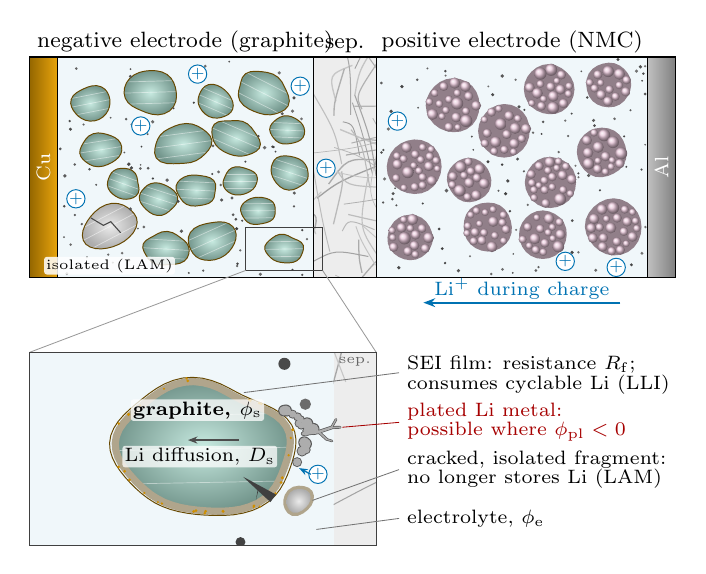
\begin{tikzpicture}[x=1mm, y=1mm, font=\footnotesize, ion/.style={circle, draw=cBlu, fill=white, line width=0.35pt, inner sep=0pt, minimum size=1.7mm, font=\tiny, text=cBlu}, lead/.style={black!55, line width=0.3pt}]
\fill[cBlu!6] (3.5,34.0) rectangle (78.5,62.0);
\fill[black!7] (36,34.0) rectangle (44,62.0);
\begin{scope}\clip (36,34.0) rectangle (44,62.0);
\draw[black!29, line width=0.41pt] (41.23,55.74) .. controls (47.96,55.75) .. (51.49,58.86);
\draw[black!28, line width=0.35pt] (39.69,39.89) .. controls (40.47,41.45) .. (43.79,40.07);
\draw[black!22, line width=0.49pt] (38.89,56.38) .. controls (37.96,59.76) .. (40.98,60.94);
\draw[black!28, line width=0.30pt] (44.60,37.31) .. controls (48.39,41.62) .. (48.43,48.35);
\draw[black!26, line width=0.32pt] (44.65,44.26) .. controls (45.20,47.90) .. (47.10,48.99);
\draw[black!31, line width=0.37pt] (40.86,51.07) .. controls (43.29,51.66) .. (47.20,52.41);
\draw[black!33, line width=0.46pt] (42.05,33.82) .. controls (45.27,37.63) .. (52.36,39.13);
\draw[black!28, line width=0.28pt] (38.66,50.51) .. controls (41.91,49.51) .. (47.18,45.96);
\draw[black!25, line width=0.40pt] (39.62,48.40) .. controls (38.79,52.58) .. (35.72,57.83);
\draw[black!33, line width=0.48pt] (37.96,45.86) .. controls (40.30,49.10) .. (43.93,48.95);
\draw[black!26, line width=0.43pt] (40.45,42.00) .. controls (44.80,40.99) .. (50.67,40.11);
\draw[black!33, line width=0.46pt] (42.20,34.59) .. controls (41.81,36.39) .. (41.77,38.82);
\draw[black!28, line width=0.28pt] (35.56,61.31) .. controls (37.99,66.09) .. (38.56,67.27);
\draw[black!23, line width=0.46pt] (41.30,57.22) .. controls (41.82,60.25) .. (43.98,63.67);
\draw[black!32, line width=0.37pt] (44.99,59.27) .. controls (41.48,64.08) .. (39.64,69.65);
\draw[black!37, line width=0.47pt] (36.47,44.06) .. controls (39.17,46.15) .. (44.43,48.29);
\draw[black!33, line width=0.42pt] (40.15,49.54) .. controls (45.95,50.59) .. (50.44,49.57);
\draw[black!31, line width=0.49pt] (38.63,54.54) .. controls (38.66,56.24) .. (39.96,60.52);
\draw[black!36, line width=0.32pt] (43.52,47.18) .. controls (42.25,52.38) .. (40.98,56.20);
\draw[black!27, line width=0.47pt] (38.57,40.76) .. controls (39.84,46.03) .. (39.61,47.48);
\draw[black!33, line width=0.48pt] (44.57,48.58) .. controls (47.27,49.43) .. (50.15,48.74);
\draw[black!30, line width=0.43pt] (42.20,55.37) .. controls (41.34,57.05) .. (44.27,61.45);
\draw[black!23, line width=0.50pt] (39.41,52.80) .. controls (45.68,50.21) .. (48.10,50.30);
\draw[black!23, line width=0.35pt] (43.92,35.55) .. controls (42.07,38.67) .. (41.42,40.50);
\draw[black!34, line width=0.49pt] (35.72,38.54) .. controls (36.71,41.96) .. (34.85,42.45);
\draw[black!38, line width=0.33pt] (41.89,49.51) .. controls (41.15,53.47) .. (39.76,53.77);
\draw[black!27, line width=0.40pt] (43.19,45.41) .. controls (42.25,50.92) .. (40.80,52.78);
\draw[black!32, line width=0.39pt] (44.68,51.48) .. controls (48.63,49.52) .. (51.66,50.43);
\draw[black!37, line width=0.32pt] (41.29,60.52) .. controls (43.92,65.90) .. (42.76,72.24);
\draw[black!31, line width=0.37pt] (44.61,61.24) .. controls (43.80,65.46) .. (43.66,71.12);
\draw[black!36, line width=0.31pt] (44.84,47.74) .. controls (43.45,48.33) .. (45.73,51.83);
\draw[black!23, line width=0.31pt] (38.92,47.37) .. controls (43.73,46.33) .. (50.39,48.06);
\draw[black!25, line width=0.25pt] (44.89,41.38) .. controls (42.95,44.56) .. (44.01,49.48);
\draw[black!33, line width=0.42pt] (42.08,51.63) .. controls (47.09,51.05) .. (49.59,53.40);
\draw[black!28, line width=0.25pt] (35.03,49.70) .. controls (41.60,50.44) .. (45.94,51.75);
\draw[black!34, line width=0.37pt] (40.76,54.66) .. controls (40.77,60.93) .. (39.32,65.44);
\draw[black!35, line width=0.40pt] (43.99,46.88) .. controls (43.22,51.94) .. (41.26,57.22);
\draw[black!26, line width=0.36pt] (38.11,37.29) .. controls (37.13,41.27) .. (35.82,48.85);
\draw[black!22, line width=0.33pt] (42.33,40.55) .. controls (46.30,36.95) .. (50.85,36.80);
\draw[black!25, line width=0.43pt] (39.05,47.57) .. controls (40.27,45.69) .. (44.40,45.46);
\draw[black!24, line width=0.41pt] (44.18,36.79) .. controls (41.78,40.40) .. (43.03,47.14);
\draw[black!26, line width=0.25pt] (38.79,34.30) .. controls (41.65,32.92) .. (47.77,30.05);
\draw[black!31, line width=0.29pt] (39.89,43.31) .. controls (42.94,43.73) .. (44.94,44.10);
\draw[black!29, line width=0.31pt] (44.10,49.76) .. controls (44.83,52.06) .. (43.56,54.23);
\draw[black!22, line width=0.41pt] (36.34,39.50) .. controls (35.03,42.87) .. (37.04,44.89);
\draw[black!36, line width=0.37pt] (35.91,35.99) .. controls (38.75,37.51) .. (43.00,36.66);
\end{scope}
\shade[left color=cOra!65!black, right color=cOra!95!white] (0,34.0) rectangle (3.5,62.0);
\shade[left color=black!25, right color=black!50] (78.5,34.0) rectangle (82,62.0);
\shade[inner color=cGre!22!white, outer color=cGre!40!black!55] plot[smooth cycle, tension=0.75] coordinates {(23.55,44.98) (23.62,45.40) (23.60,45.87) (23.37,46.32) (22.92,46.65) (22.36,46.83) (21.79,46.92) (21.25,46.99) (20.69,47.01) (20.13,46.94) (19.60,46.75) (19.15,46.46) (18.80,46.10) (18.60,45.67) (18.59,45.21) (18.74,44.78) (18.95,44.38) (19.18,44.00) (19.48,43.61) (19.91,43.28) (20.47,43.10) (21.06,43.07) (21.63,43.14) (22.19,43.24) (22.73,43.41) (23.16,43.72) (23.41,44.13) (23.49,44.56)};
\begin{scope}\clip plot[smooth cycle, tension=0.75] coordinates {(23.55,44.98) (23.62,45.40) (23.60,45.87) (23.37,46.32) (22.92,46.65) (22.36,46.83) (21.79,46.92) (21.25,46.99) (20.69,47.01) (20.13,46.94) (19.60,46.75) (19.15,46.46) (18.80,46.10) (18.60,45.67) (18.59,45.21) (18.74,44.78) (18.95,44.38) (19.18,44.00) (19.48,43.61) (19.91,43.28) (20.47,43.10) (21.06,43.07) (21.63,43.14) (22.19,43.24) (22.73,43.41) (23.16,43.72) (23.41,44.13) (23.49,44.56)};
\draw[white, opacity=0.45, line width=0.25pt] (17.65,44.22) -- (24.57,43.89);
\draw[white, opacity=0.45, line width=0.25pt] (17.70,45.25) -- (24.62,44.92);
\draw[white, opacity=0.45, line width=0.25pt] (17.75,46.29) -- (24.67,45.96);
\end{scope}
\draw[cOra!45!black, line width=0.35pt] plot[smooth cycle, tension=0.75] coordinates {(23.55,44.98) (23.62,45.40) (23.60,45.87) (23.37,46.32) (22.92,46.65) (22.36,46.83) (21.79,46.92) (21.25,46.99) (20.69,47.01) (20.13,46.94) (19.60,46.75) (19.15,46.46) (18.80,46.10) (18.60,45.67) (18.59,45.21) (18.74,44.78) (18.95,44.38) (19.18,44.00) (19.48,43.61) (19.91,43.28) (20.47,43.10) (21.06,43.07) (21.63,43.14) (22.19,43.24) (22.73,43.41) (23.16,43.72) (23.41,44.13) (23.49,44.56)};
\shade[inner color=cGre!22!white, outer color=cGre!40!black!55] plot[smooth cycle, tension=0.75] coordinates {(26.09,40.01) (25.78,40.48) (25.30,40.83) (24.72,41.02) (24.08,41.07) (23.46,41.01) (22.85,40.92) (22.22,40.79) (21.55,40.59) (20.90,40.24) (20.40,39.72) (20.15,39.11) (20.13,38.50) (20.27,37.96) (20.48,37.47) (20.75,37.03) (21.13,36.64) (21.63,36.36) (22.22,36.21) (22.86,36.17) (23.52,36.25) (24.18,36.47) (24.78,36.81) (25.28,37.25) (25.68,37.76) (25.98,38.30) (26.17,38.87) (26.22,39.45)};
\begin{scope}\clip plot[smooth cycle, tension=0.75] coordinates {(26.09,40.01) (25.78,40.48) (25.30,40.83) (24.72,41.02) (24.08,41.07) (23.46,41.01) (22.85,40.92) (22.22,40.79) (21.55,40.59) (20.90,40.24) (20.40,39.72) (20.15,39.11) (20.13,38.50) (20.27,37.96) (20.48,37.47) (20.75,37.03) (21.13,36.64) (21.63,36.36) (22.22,36.21) (22.86,36.17) (23.52,36.25) (24.18,36.47) (24.78,36.81) (25.28,37.25) (25.68,37.76) (25.98,38.30) (26.17,38.87) (26.22,39.45)};
\draw[white, opacity=0.45, line width=0.25pt] (19.88,35.83) -- (27.50,39.27);
\draw[white, opacity=0.45, line width=0.25pt] (19.36,36.97) -- (26.98,40.41);
\draw[white, opacity=0.45, line width=0.25pt] (18.85,38.11) -- (26.46,41.55);
\end{scope}
\draw[cOra!45!black, line width=0.35pt] plot[smooth cycle, tension=0.75] coordinates {(26.09,40.01) (25.78,40.48) (25.30,40.83) (24.72,41.02) (24.08,41.07) (23.46,41.01) (22.85,40.92) (22.22,40.79) (21.55,40.59) (20.90,40.24) (20.40,39.72) (20.15,39.11) (20.13,38.50) (20.27,37.96) (20.48,37.47) (20.75,37.03) (21.13,36.64) (21.63,36.36) (22.22,36.21) (22.86,36.17) (23.52,36.25) (24.18,36.47) (24.78,36.81) (25.28,37.25) (25.68,37.76) (25.98,38.30) (26.17,38.87) (26.22,39.45)};
\shade[inner color=cGre!22!white, outer color=cGre!40!black!55] plot[smooth cycle, tension=0.75] coordinates {(31.18,42.49) (31.17,42.87) (31.08,43.25) (30.85,43.61) (30.47,43.88) (30.01,44.06) (29.52,44.16) (29.02,44.19) (28.52,44.15) (28.05,44.02) (27.63,43.81) (27.26,43.54) (26.97,43.22) (26.80,42.85) (26.79,42.46) (26.90,42.08) (27.08,41.73) (27.30,41.39) (27.60,41.07) (28.02,40.83) (28.53,40.73) (29.05,40.76) (29.53,40.84) (30.00,40.94) (30.47,41.11) (30.85,41.37) (31.08,41.73) (31.17,42.12)};
\begin{scope}\clip plot[smooth cycle, tension=0.75] coordinates {(31.18,42.49) (31.17,42.87) (31.08,43.25) (30.85,43.61) (30.47,43.88) (30.01,44.06) (29.52,44.16) (29.02,44.19) (28.52,44.15) (28.05,44.02) (27.63,43.81) (27.26,43.54) (26.97,43.22) (26.80,42.85) (26.79,42.46) (26.90,42.08) (27.08,41.73) (27.30,41.39) (27.60,41.07) (28.02,40.83) (28.53,40.73) (29.05,40.76) (29.53,40.84) (30.00,40.94) (30.47,41.11) (30.85,41.37) (31.08,41.73) (31.17,42.12)};
\draw[white, opacity=0.45, line width=0.25pt] (26.01,41.54) -- (32.07,41.59);
\draw[white, opacity=0.45, line width=0.25pt] (26.01,42.45) -- (32.06,42.50);
\draw[white, opacity=0.45, line width=0.25pt] (26.00,43.36) -- (32.05,43.40);
\end{scope}
\draw[cOra!45!black, line width=0.35pt] plot[smooth cycle, tension=0.75] coordinates {(31.18,42.49) (31.17,42.87) (31.08,43.25) (30.85,43.61) (30.47,43.88) (30.01,44.06) (29.52,44.16) (29.02,44.19) (28.52,44.15) (28.05,44.02) (27.63,43.81) (27.26,43.54) (26.97,43.22) (26.80,42.85) (26.79,42.46) (26.90,42.08) (27.08,41.73) (27.30,41.39) (27.60,41.07) (28.02,40.83) (28.53,40.73) (29.05,40.76) (29.53,40.84) (30.00,40.94) (30.47,41.11) (30.85,41.37) (31.08,41.73) (31.17,42.12)};
\shade[inner color=cGre!22!white, outer color=cGre!40!black!55] plot[smooth cycle, tension=0.75] coordinates {(35.31,46.57) (35.37,47.00) (35.33,47.44) (35.23,47.89) (35.02,48.34) (34.66,48.76) (34.17,49.07) (33.61,49.27) (33.05,49.39) (32.47,49.45) (31.90,49.41) (31.40,49.22) (31.04,48.89) (30.83,48.49) (30.70,48.08) (30.65,47.66) (30.69,47.23) (30.83,46.80) (31.05,46.38) (31.35,45.95) (31.76,45.54) (32.29,45.22) (32.91,45.09) (33.50,45.16) (34.00,45.37) (34.42,45.62) (34.80,45.88) (35.12,46.19)};
\begin{scope}\clip plot[smooth cycle, tension=0.75] coordinates {(35.31,46.57) (35.37,47.00) (35.33,47.44) (35.23,47.89) (35.02,48.34) (34.66,48.76) (34.17,49.07) (33.61,49.27) (33.05,49.39) (32.47,49.45) (31.90,49.41) (31.40,49.22) (31.04,48.89) (30.83,48.49) (30.70,48.08) (30.65,47.66) (30.69,47.23) (30.83,46.80) (31.05,46.38) (31.35,45.95) (31.76,45.54) (32.29,45.22) (32.91,45.09) (33.50,45.16) (34.00,45.37) (34.42,45.62) (34.80,45.88) (35.12,46.19)};
\draw[white, opacity=0.45, line width=0.25pt] (29.37,47.42) -- (35.95,45.28);
\draw[white, opacity=0.45, line width=0.25pt] (29.69,48.41) -- (36.27,46.26);
\draw[white, opacity=0.45, line width=0.25pt] (30.02,49.39) -- (36.59,47.25);
\end{scope}
\draw[cOra!45!black, line width=0.35pt] plot[smooth cycle, tension=0.75] coordinates {(35.31,46.57) (35.37,47.00) (35.33,47.44) (35.23,47.89) (35.02,48.34) (34.66,48.76) (34.17,49.07) (33.61,49.27) (33.05,49.39) (32.47,49.45) (31.90,49.41) (31.40,49.22) (31.04,48.89) (30.83,48.49) (30.70,48.08) (30.65,47.66) (30.69,47.23) (30.83,46.80) (31.05,46.38) (31.35,45.95) (31.76,45.54) (32.29,45.22) (32.91,45.09) (33.50,45.16) (34.00,45.37) (34.42,45.62) (34.80,45.88) (35.12,46.19)};
\shade[inner color=cGre!22!white, outer color=cGre!40!black!55] plot[smooth cycle, tension=0.75] coordinates {(23.14,51.38) (22.92,51.97) (22.47,52.46) (21.93,52.87) (21.34,53.22) (20.65,53.48) (19.87,53.56) (19.08,53.45) (18.36,53.21) (17.70,52.91) (17.09,52.56) (16.59,52.10) (16.26,51.58) (16.05,51.02) (15.91,50.44) (15.86,49.80) (16.06,49.18) (16.61,48.70) (17.41,48.47) (18.24,48.44) (19.01,48.47) (19.73,48.51) (20.46,48.60) (21.16,48.85) (21.75,49.23) (22.26,49.68) (22.71,50.18) (23.05,50.76)};
\begin{scope}\clip plot[smooth cycle, tension=0.75] coordinates {(23.14,51.38) (22.92,51.97) (22.47,52.46) (21.93,52.87) (21.34,53.22) (20.65,53.48) (19.87,53.56) (19.08,53.45) (18.36,53.21) (17.70,52.91) (17.09,52.56) (16.59,52.10) (16.26,51.58) (16.05,51.02) (15.91,50.44) (15.86,49.80) (16.06,49.18) (16.61,48.70) (17.41,48.47) (18.24,48.44) (19.01,48.47) (19.73,48.51) (20.46,48.60) (21.16,48.85) (21.75,49.23) (22.26,49.68) (22.71,50.18) (23.05,50.76)};
\draw[white, opacity=0.45, line width=0.25pt] (15.01,48.92) -- (24.19,50.12);
\draw[white, opacity=0.45, line width=0.25pt] (14.83,50.30) -- (24.01,51.50);
\draw[white, opacity=0.45, line width=0.25pt] (14.65,51.67) -- (23.83,52.87);
\end{scope}
\draw[cOra!45!black, line width=0.35pt] plot[smooth cycle, tension=0.75] coordinates {(23.14,51.38) (22.92,51.97) (22.47,52.46) (21.93,52.87) (21.34,53.22) (20.65,53.48) (19.87,53.56) (19.08,53.45) (18.36,53.21) (17.70,52.91) (17.09,52.56) (16.59,52.10) (16.26,51.58) (16.05,51.02) (15.91,50.44) (15.86,49.80) (16.06,49.18) (16.61,48.70) (17.41,48.47) (18.24,48.44) (19.01,48.47) (19.73,48.51) (20.46,48.60) (21.16,48.85) (21.75,49.23) (22.26,49.68) (22.71,50.18) (23.05,50.76)};
\shade[inner color=cGre!22!white, outer color=cGre!40!black!55] plot[smooth cycle, tension=0.75] coordinates {(25.77,55.37) (25.85,55.81) (25.79,56.25) (25.63,56.68) (25.41,57.08) (25.12,57.46) (24.76,57.81) (24.34,58.13) (23.84,58.39) (23.28,58.54) (22.72,58.50) (22.25,58.28) (21.92,57.95) (21.69,57.57) (21.53,57.20) (21.41,56.81) (21.37,56.39) (21.45,55.96) (21.64,55.53) (21.92,55.12) (22.29,54.74) (22.75,54.44) (23.29,54.27) (23.83,54.24) (24.33,54.32) (24.79,54.48) (25.21,54.69) (25.55,54.99)};
\begin{scope}\clip plot[smooth cycle, tension=0.75] coordinates {(25.77,55.37) (25.85,55.81) (25.79,56.25) (25.63,56.68) (25.41,57.08) (25.12,57.46) (24.76,57.81) (24.34,58.13) (23.84,58.39) (23.28,58.54) (22.72,58.50) (22.25,58.28) (21.92,57.95) (21.69,57.57) (21.53,57.20) (21.41,56.81) (21.37,56.39) (21.45,55.96) (21.64,55.53) (21.92,55.12) (22.29,54.74) (22.75,54.44) (23.29,54.27) (23.83,54.24) (24.33,54.32) (24.79,54.48) (25.21,54.69) (25.55,54.99)};
\draw[white, opacity=0.45, line width=0.25pt] (20.15,56.71) -- (26.20,54.11);
\draw[white, opacity=0.45, line width=0.25pt] (20.54,57.62) -- (26.59,55.02);
\draw[white, opacity=0.45, line width=0.25pt] (20.93,58.53) -- (26.98,55.93);
\end{scope}
\draw[cOra!45!black, line width=0.35pt] plot[smooth cycle, tension=0.75] coordinates {(25.77,55.37) (25.85,55.81) (25.79,56.25) (25.63,56.68) (25.41,57.08) (25.12,57.46) (24.76,57.81) (24.34,58.13) (23.84,58.39) (23.28,58.54) (22.72,58.50) (22.25,58.28) (21.92,57.95) (21.69,57.57) (21.53,57.20) (21.41,56.81) (21.37,56.39) (21.45,55.96) (21.64,55.53) (21.92,55.12) (22.29,54.74) (22.75,54.44) (23.29,54.27) (23.83,54.24) (24.33,54.32) (24.79,54.48) (25.21,54.69) (25.55,54.99)};
\shade[inner color=cGre!22!white, outer color=cGre!40!black!55] plot[smooth cycle, tension=0.75] coordinates {(29.15,50.40) (29.30,50.93) (29.17,51.51) (28.85,52.05) (28.51,52.54) (28.15,53.04) (27.67,53.50) (27.05,53.82) (26.38,53.93) (25.76,53.91) (25.18,53.89) (24.56,53.87) (23.94,53.77) (23.44,53.46) (23.18,52.99) (23.13,52.45) (23.19,51.91) (23.34,51.36) (23.63,50.83) (24.09,50.36) (24.66,49.98) (25.27,49.70) (25.89,49.50) (26.53,49.41) (27.14,49.43) (27.70,49.56) (28.23,49.75) (28.74,50.01)};
\begin{scope}\clip plot[smooth cycle, tension=0.75] coordinates {(29.15,50.40) (29.30,50.93) (29.17,51.51) (28.85,52.05) (28.51,52.54) (28.15,53.04) (27.67,53.50) (27.05,53.82) (26.38,53.93) (25.76,53.91) (25.18,53.89) (24.56,53.87) (23.94,53.77) (23.44,53.46) (23.18,52.99) (23.13,52.45) (23.19,51.91) (23.34,51.36) (23.63,50.83) (24.09,50.36) (24.66,49.98) (25.27,49.70) (25.89,49.50) (26.53,49.41) (27.14,49.43) (27.70,49.56) (28.23,49.75) (28.74,50.01)};
\draw[white, opacity=0.45, line width=0.25pt] (21.97,52.20) -- (29.35,49.00);
\draw[white, opacity=0.45, line width=0.25pt] (22.45,53.31) -- (29.83,50.11);
\draw[white, opacity=0.45, line width=0.25pt] (22.93,54.42) -- (30.31,51.22);
\end{scope}
\draw[cOra!45!black, line width=0.35pt] plot[smooth cycle, tension=0.75] coordinates {(29.15,50.40) (29.30,50.93) (29.17,51.51) (28.85,52.05) (28.51,52.54) (28.15,53.04) (27.67,53.50) (27.05,53.82) (26.38,53.93) (25.76,53.91) (25.18,53.89) (24.56,53.87) (23.94,53.77) (23.44,53.46) (23.18,52.99) (23.13,52.45) (23.19,51.91) (23.34,51.36) (23.63,50.83) (24.09,50.36) (24.66,49.98) (25.27,49.70) (25.89,49.50) (26.53,49.41) (27.14,49.43) (27.70,49.56) (28.23,49.75) (28.74,50.01)};
\shade[inner color=cGre!22!white, outer color=cGre!40!black!55] plot[smooth cycle, tension=0.75] coordinates {(10.18,56.59) (10.07,57.05) (9.87,57.50) (9.55,57.91) (9.09,58.21) (8.53,58.36) (7.94,58.34) (7.39,58.19) (6.89,57.98) (6.42,57.75) (5.95,57.47) (5.53,57.10) (5.27,56.63) (5.20,56.12) (5.32,55.64) (5.55,55.20) (5.84,54.82) (6.18,54.47) (6.60,54.18) (7.09,53.96) (7.65,53.86) (8.24,53.89) (8.80,54.07) (9.28,54.37) (9.67,54.76) (9.94,55.19) (10.11,55.65) (10.19,56.12)};
\begin{scope}\clip plot[smooth cycle, tension=0.75] coordinates {(10.18,56.59) (10.07,57.05) (9.87,57.50) (9.55,57.91) (9.09,58.21) (8.53,58.36) (7.94,58.34) (7.39,58.19) (6.89,57.98) (6.42,57.75) (5.95,57.47) (5.53,57.10) (5.27,56.63) (5.20,56.12) (5.32,55.64) (5.55,55.20) (5.84,54.82) (6.18,54.47) (6.60,54.18) (7.09,53.96) (7.65,53.86) (8.24,53.89) (8.80,54.07) (9.28,54.37) (9.67,54.76) (9.94,55.19) (10.11,55.65) (10.19,56.12)};
\draw[white, opacity=0.45, line width=0.25pt] (4.48,54.38) -- (11.53,55.75);
\draw[white, opacity=0.45, line width=0.25pt] (4.28,55.43) -- (11.32,56.81);
\draw[white, opacity=0.45, line width=0.25pt] (4.07,56.49) -- (11.11,57.87);
\end{scope}
\draw[cOra!45!black, line width=0.35pt] plot[smooth cycle, tension=0.75] coordinates {(10.18,56.59) (10.07,57.05) (9.87,57.50) (9.55,57.91) (9.09,58.21) (8.53,58.36) (7.94,58.34) (7.39,58.19) (6.89,57.98) (6.42,57.75) (5.95,57.47) (5.53,57.10) (5.27,56.63) (5.20,56.12) (5.32,55.64) (5.55,55.20) (5.84,54.82) (6.18,54.47) (6.60,54.18) (7.09,53.96) (7.65,53.86) (8.24,53.89) (8.80,54.07) (9.28,54.37) (9.67,54.76) (9.94,55.19) (10.11,55.65) (10.19,56.12)};
\shade[inner color=black!8, outer color=black!32] plot[smooth cycle, tension=0.75] coordinates {(13.27,42.10) (12.88,42.52) (12.42,42.88) (11.87,43.19) (11.22,43.39) (10.45,43.42) (9.64,43.22) (8.89,42.83) (8.26,42.32) (7.75,41.76) (7.33,41.18) (7.00,40.58) (6.76,39.95) (6.68,39.32) (6.80,38.71) (7.14,38.21) (7.68,37.86) (8.35,37.67) (9.08,37.63) (9.83,37.72) (10.58,37.91) (11.31,38.20) (12.01,38.60) (12.63,39.10) (13.15,39.68) (13.50,40.33) (13.65,40.99) (13.56,41.59)};
\begin{scope}\clip plot[smooth cycle, tension=0.75] coordinates {(13.27,42.10) (12.88,42.52) (12.42,42.88) (11.87,43.19) (11.22,43.39) (10.45,43.42) (9.64,43.22) (8.89,42.83) (8.26,42.32) (7.75,41.76) (7.33,41.18) (7.00,40.58) (6.76,39.95) (6.68,39.32) (6.80,38.71) (7.14,38.21) (7.68,37.86) (8.35,37.67) (9.08,37.63) (9.83,37.72) (10.58,37.91) (11.31,38.20) (12.01,38.60) (12.63,39.10) (13.15,39.68) (13.50,40.33) (13.65,40.99) (13.56,41.59)};
\draw[white, opacity=0.5, line width=0.25pt] (6.61,37.02) -- (14.96,41.39);
\draw[white, opacity=0.5, line width=0.25pt] (5.96,38.27) -- (14.31,42.65);
\draw[white, opacity=0.5, line width=0.25pt] (5.30,39.53) -- (13.65,43.90);
\end{scope}
\draw[cOra!45!black, line width=0.35pt] plot[smooth cycle, tension=0.75] coordinates {(13.27,42.10) (12.88,42.52) (12.42,42.88) (11.87,43.19) (11.22,43.39) (10.45,43.42) (9.64,43.22) (8.89,42.83) (8.26,42.32) (7.75,41.76) (7.33,41.18) (7.00,40.58) (6.76,39.95) (6.68,39.32) (6.80,38.71) (7.14,38.21) (7.68,37.86) (8.35,37.67) (9.08,37.63) (9.83,37.72) (10.58,37.91) (11.31,38.20) (12.01,38.60) (12.63,39.10) (13.15,39.68) (13.50,40.33) (13.65,40.99) (13.56,41.59)};
\draw[black!70, line width=0.4pt] (7.77,41.56) -- (9.35,40.62) -- (10.29,41.09) -- (11.55,39.67);
\shade[inner color=cGre!22!white, outer color=cGre!40!black!55] plot[smooth cycle, tension=0.75] coordinates {(11.67,50.63) (11.52,51.07) (11.24,51.46) (10.83,51.76) (10.35,51.99) (9.84,52.16) (9.29,52.30) (8.67,52.36) (8.04,52.25) (7.49,51.96) (7.10,51.55) (6.82,51.12) (6.59,50.70) (6.40,50.26) (6.35,49.80) (6.49,49.36) (6.78,48.98) (7.16,48.65) (7.59,48.36) (8.11,48.14) (8.71,48.06) (9.33,48.14) (9.89,48.34) (10.41,48.59) (10.88,48.89) (11.29,49.26) (11.57,49.69) (11.69,50.16)};
\begin{scope}\clip plot[smooth cycle, tension=0.75] coordinates {(11.67,50.63) (11.52,51.07) (11.24,51.46) (10.83,51.76) (10.35,51.99) (9.84,52.16) (9.29,52.30) (8.67,52.36) (8.04,52.25) (7.49,51.96) (7.10,51.55) (6.82,51.12) (6.59,50.70) (6.40,50.26) (6.35,49.80) (6.49,49.36) (6.78,48.98) (7.16,48.65) (7.59,48.36) (8.11,48.14) (8.71,48.06) (9.33,48.14) (9.89,48.34) (10.41,48.59) (10.88,48.89) (11.29,49.26) (11.57,49.69) (11.69,50.16)};
\draw[white, opacity=0.45, line width=0.25pt] (5.61,48.59) -- (12.73,49.70);
\draw[white, opacity=0.45, line width=0.25pt] (5.44,49.66) -- (12.56,50.77);
\draw[white, opacity=0.45, line width=0.25pt] (5.28,50.73) -- (12.40,51.84);
\end{scope}
\draw[cOra!45!black, line width=0.35pt] plot[smooth cycle, tension=0.75] coordinates {(11.67,50.63) (11.52,51.07) (11.24,51.46) (10.83,51.76) (10.35,51.99) (9.84,52.16) (9.29,52.30) (8.67,52.36) (8.04,52.25) (7.49,51.96) (7.10,51.55) (6.82,51.12) (6.59,50.70) (6.40,50.26) (6.35,49.80) (6.49,49.36) (6.78,48.98) (7.16,48.65) (7.59,48.36) (8.11,48.14) (8.71,48.06) (9.33,48.14) (9.89,48.34) (10.41,48.59) (10.88,48.89) (11.29,49.26) (11.57,49.69) (11.69,50.16)};
\shade[inner color=cGre!22!white, outer color=cGre!40!black!55] plot[smooth cycle, tension=0.75] coordinates {(13.88,45.19) (13.83,45.61) (13.74,45.99) (13.69,46.37) (13.61,46.78) (13.42,47.21) (13.05,47.56) (12.58,47.77) (12.08,47.86) (11.59,47.86) (11.11,47.78) (10.70,47.58) (10.38,47.28) (10.17,46.93) (10.02,46.57) (9.90,46.19) (9.86,45.78) (9.95,45.36) (10.17,44.97) (10.49,44.63) (10.86,44.35) (11.28,44.12) (11.75,43.97) (12.24,43.93) (12.72,43.99) (13.17,44.14) (13.55,44.40) (13.80,44.77)};
\begin{scope}\clip plot[smooth cycle, tension=0.75] coordinates {(13.88,45.19) (13.83,45.61) (13.74,45.99) (13.69,46.37) (13.61,46.78) (13.42,47.21) (13.05,47.56) (12.58,47.77) (12.08,47.86) (11.59,47.86) (11.11,47.78) (10.70,47.58) (10.38,47.28) (10.17,46.93) (10.02,46.57) (9.90,46.19) (9.86,45.78) (9.95,45.36) (10.17,44.97) (10.49,44.63) (10.86,44.35) (11.28,44.12) (11.75,43.97) (12.24,43.93) (12.72,43.99) (13.17,44.14) (13.55,44.40) (13.80,44.77)};
\draw[white, opacity=0.45, line width=0.25pt] (8.72,46.05) -- (14.49,44.00);
\draw[white, opacity=0.45, line width=0.25pt] (9.03,46.92) -- (14.80,44.86);
\draw[white, opacity=0.45, line width=0.25pt] (9.34,47.78) -- (15.11,45.73);
\end{scope}
\draw[cOra!45!black, line width=0.35pt] plot[smooth cycle, tension=0.75] coordinates {(13.88,45.19) (13.83,45.61) (13.74,45.99) (13.69,46.37) (13.61,46.78) (13.42,47.21) (13.05,47.56) (12.58,47.77) (12.08,47.86) (11.59,47.86) (11.11,47.78) (10.70,47.58) (10.38,47.28) (10.17,46.93) (10.02,46.57) (9.90,46.19) (9.86,45.78) (9.95,45.36) (10.17,44.97) (10.49,44.63) (10.86,44.35) (11.28,44.12) (11.75,43.97) (12.24,43.93) (12.72,43.99) (13.17,44.14) (13.55,44.40) (13.80,44.77)};
\shade[inner color=cGre!22!white, outer color=cGre!40!black!55] plot[smooth cycle, tension=0.75] coordinates {(18.60,57.60) (18.48,58.20) (18.27,58.78) (17.93,59.33) (17.43,59.79) (16.79,60.10) (16.08,60.25) (15.35,60.28) (14.63,60.21) (13.92,60.04) (13.25,59.73) (12.69,59.28) (12.28,58.71) (12.04,58.08) (11.98,57.42) (12.13,56.77) (12.49,56.20) (13.02,55.76) (13.61,55.44) (14.21,55.18) (14.82,54.93) (15.51,54.73) (16.28,54.65) (17.07,54.79) (17.76,55.15) (18.26,55.69) (18.55,56.33) (18.64,56.98)};
\begin{scope}\clip plot[smooth cycle, tension=0.75] coordinates {(18.60,57.60) (18.48,58.20) (18.27,58.78) (17.93,59.33) (17.43,59.79) (16.79,60.10) (16.08,60.25) (15.35,60.28) (14.63,60.21) (13.92,60.04) (13.25,59.73) (12.69,59.28) (12.28,58.71) (12.04,58.08) (11.98,57.42) (12.13,56.77) (12.49,56.20) (13.02,55.76) (13.61,55.44) (14.21,55.18) (14.82,54.93) (15.51,54.73) (16.28,54.65) (17.07,54.79) (17.76,55.15) (18.26,55.69) (18.55,56.33) (18.64,56.98)};
\draw[white, opacity=0.45, line width=0.25pt] (10.78,55.97) -- (20.16,56.24);
\draw[white, opacity=0.45, line width=0.25pt] (10.74,57.38) -- (20.12,57.65);
\draw[white, opacity=0.45, line width=0.25pt] (10.70,58.79) -- (20.08,59.05);
\end{scope}
\draw[cOra!45!black, line width=0.35pt] plot[smooth cycle, tension=0.75] coordinates {(18.60,57.60) (18.48,58.20) (18.27,58.78) (17.93,59.33) (17.43,59.79) (16.79,60.10) (16.08,60.25) (15.35,60.28) (14.63,60.21) (13.92,60.04) (13.25,59.73) (12.69,59.28) (12.28,58.71) (12.04,58.08) (11.98,57.42) (12.13,56.77) (12.49,56.20) (13.02,55.76) (13.61,55.44) (14.21,55.18) (14.82,54.93) (15.51,54.73) (16.28,54.65) (17.07,54.79) (17.76,55.15) (18.26,55.69) (18.55,56.33) (18.64,56.98)};
\shade[inner color=cGre!22!white, outer color=cGre!40!black!55] plot[smooth cycle, tension=0.75] coordinates {(18.56,43.27) (18.76,43.68) (18.79,44.16) (18.63,44.63) (18.29,45.04) (17.86,45.37) (17.40,45.63) (16.92,45.84) (16.40,45.99) (15.87,46.02) (15.37,45.92) (14.94,45.70) (14.60,45.41) (14.30,45.08) (14.05,44.71) (13.92,44.29) (13.95,43.82) (14.15,43.38) (14.45,42.98) (14.80,42.62) (15.21,42.28) (15.69,42.01) (16.24,41.87) (16.79,41.90) (17.26,42.09) (17.64,42.35) (17.96,42.64) (18.27,42.93)};
\begin{scope}\clip plot[smooth cycle, tension=0.75] coordinates {(18.56,43.27) (18.76,43.68) (18.79,44.16) (18.63,44.63) (18.29,45.04) (17.86,45.37) (17.40,45.63) (16.92,45.84) (16.40,45.99) (15.87,46.02) (15.37,45.92) (14.94,45.70) (14.60,45.41) (14.30,45.08) (14.05,44.71) (13.92,44.29) (13.95,43.82) (14.15,43.38) (14.45,42.98) (14.80,42.62) (15.21,42.28) (15.69,42.01) (16.24,41.87) (16.79,41.90) (17.26,42.09) (17.64,42.35) (17.96,42.64) (18.27,42.93)};
\draw[white, opacity=0.45, line width=0.25pt] (12.84,44.05) -- (19.20,42.02);
\draw[white, opacity=0.45, line width=0.25pt] (13.15,45.00) -- (19.50,42.97);
\draw[white, opacity=0.45, line width=0.25pt] (13.45,45.96) -- (19.81,43.92);
\end{scope}
\draw[cOra!45!black, line width=0.35pt] plot[smooth cycle, tension=0.75] coordinates {(18.56,43.27) (18.76,43.68) (18.79,44.16) (18.63,44.63) (18.29,45.04) (17.86,45.37) (17.40,45.63) (16.92,45.84) (16.40,45.99) (15.87,46.02) (15.37,45.92) (14.94,45.70) (14.60,45.41) (14.30,45.08) (14.05,44.71) (13.92,44.29) (13.95,43.82) (14.15,43.38) (14.45,42.98) (14.80,42.62) (15.21,42.28) (15.69,42.01) (16.24,41.87) (16.79,41.90) (17.26,42.09) (17.64,42.35) (17.96,42.64) (18.27,42.93)};
\shade[inner color=cGre!22!white, outer color=cGre!40!black!55] plot[smooth cycle, tension=0.75] coordinates {(32.82,55.80) (32.97,56.40) (32.86,57.06) (32.61,57.67) (32.33,58.25) (32.02,58.85) (31.55,59.41) (30.90,59.82) (30.17,60.04) (29.45,60.14) (28.74,60.19) (28.03,60.14) (27.41,59.88) (27.01,59.41) (26.82,58.84) (26.69,58.29) (26.54,57.73) (26.48,57.10) (26.68,56.44) (27.16,55.85) (27.81,55.41) (28.50,55.09) (29.18,54.85) (29.88,54.68) (30.57,54.66) (31.23,54.78) (31.85,55.00) (32.41,55.32)};
\begin{scope}\clip plot[smooth cycle, tension=0.75] coordinates {(32.82,55.80) (32.97,56.40) (32.86,57.06) (32.61,57.67) (32.33,58.25) (32.02,58.85) (31.55,59.41) (30.90,59.82) (30.17,60.04) (29.45,60.14) (28.74,60.19) (28.03,60.14) (27.41,59.88) (27.01,59.41) (26.82,58.84) (26.69,58.29) (26.54,57.73) (26.48,57.10) (26.68,56.44) (27.16,55.85) (27.81,55.41) (28.50,55.09) (29.18,54.85) (29.88,54.68) (30.57,54.66) (31.23,54.78) (31.85,55.00) (32.41,55.32)};
\draw[white, opacity=0.45, line width=0.25pt] (24.98,58.24) -- (33.12,54.11);
\draw[white, opacity=0.45, line width=0.25pt] (25.60,59.46) -- (33.74,55.33);
\draw[white, opacity=0.45, line width=0.25pt] (26.22,60.69) -- (34.36,56.55);
\end{scope}
\draw[cOra!45!black, line width=0.35pt] plot[smooth cycle, tension=0.75] coordinates {(32.82,55.80) (32.97,56.40) (32.86,57.06) (32.61,57.67) (32.33,58.25) (32.02,58.85) (31.55,59.41) (30.90,59.82) (30.17,60.04) (29.45,60.14) (28.74,60.19) (28.03,60.14) (27.41,59.88) (27.01,59.41) (26.82,58.84) (26.69,58.29) (26.54,57.73) (26.48,57.10) (26.68,56.44) (27.16,55.85) (27.81,55.41) (28.50,55.09) (29.18,54.85) (29.88,54.68) (30.57,54.66) (31.23,54.78) (31.85,55.00) (32.41,55.32)};
\shade[inner color=cGre!22!white, outer color=cGre!40!black!55] plot[smooth cycle, tension=0.75] coordinates {(20.25,37.44) (20.18,37.91) (19.94,38.36) (19.56,38.74) (19.13,39.07) (18.67,39.40) (18.13,39.70) (17.47,39.85) (16.80,39.79) (16.23,39.55) (15.74,39.27) (15.25,39.01) (14.76,38.70) (14.42,38.28) (14.35,37.79) (14.50,37.31) (14.75,36.86) (15.02,36.43) (15.40,36.02) (15.94,35.73) (16.58,35.61) (17.22,35.61) (17.82,35.64) (18.45,35.68) (19.08,35.80) (19.63,36.08) (20.00,36.49) (20.19,36.95)};
\begin{scope}\clip plot[smooth cycle, tension=0.75] coordinates {(20.25,37.44) (20.18,37.91) (19.94,38.36) (19.56,38.74) (19.13,39.07) (18.67,39.40) (18.13,39.70) (17.47,39.85) (16.80,39.79) (16.23,39.55) (15.74,39.27) (15.25,39.01) (14.76,38.70) (14.42,38.28) (14.35,37.79) (14.50,37.31) (14.75,36.86) (15.02,36.43) (15.40,36.02) (15.94,35.73) (16.58,35.61) (17.22,35.61) (17.82,35.64) (18.45,35.68) (19.08,35.80) (19.63,36.08) (20.00,36.49) (20.19,36.95)};
\draw[white, opacity=0.45, line width=0.25pt] (13.49,36.70) -- (21.05,36.25);
\draw[white, opacity=0.45, line width=0.25pt] (13.56,37.83) -- (21.12,37.38);
\draw[white, opacity=0.45, line width=0.25pt] (13.63,38.97) -- (21.18,38.52);
\end{scope}
\draw[cOra!45!black, line width=0.35pt] plot[smooth cycle, tension=0.75] coordinates {(20.25,37.44) (20.18,37.91) (19.94,38.36) (19.56,38.74) (19.13,39.07) (18.67,39.40) (18.13,39.70) (17.47,39.85) (16.80,39.79) (16.23,39.55) (15.74,39.27) (15.25,39.01) (14.76,38.70) (14.42,38.28) (14.35,37.79) (14.50,37.31) (14.75,36.86) (15.02,36.43) (15.40,36.02) (15.94,35.73) (16.58,35.61) (17.22,35.61) (17.82,35.64) (18.45,35.68) (19.08,35.80) (19.63,36.08) (20.00,36.49) (20.19,36.95)};
\shade[inner color=cGre!22!white, outer color=cGre!40!black!55] plot[smooth cycle, tension=0.75] coordinates {(34.77,37.66) (34.74,38.08) (34.49,38.45) (34.07,38.72) (33.62,38.90) (33.22,39.08) (32.81,39.31) (32.30,39.48) (31.74,39.48) (31.23,39.30) (30.81,39.02) (30.44,38.71) (30.10,38.38) (29.87,37.99) (29.85,37.57) (30.03,37.17) (30.30,36.82) (30.60,36.51) (30.95,36.24) (31.38,36.04) (31.86,35.92) (32.37,35.86) (32.90,35.85) (33.45,35.92) (33.94,36.13) (34.30,36.46) (34.52,36.86) (34.67,37.25)};
\begin{scope}\clip plot[smooth cycle, tension=0.75] coordinates {(34.77,37.66) (34.74,38.08) (34.49,38.45) (34.07,38.72) (33.62,38.90) (33.22,39.08) (32.81,39.31) (32.30,39.48) (31.74,39.48) (31.23,39.30) (30.81,39.02) (30.44,38.71) (30.10,38.38) (29.87,37.99) (29.85,37.57) (30.03,37.17) (30.30,36.82) (30.60,36.51) (30.95,36.24) (31.38,36.04) (31.86,35.92) (32.37,35.86) (32.90,35.85) (33.45,35.92) (33.94,36.13) (34.30,36.46) (34.52,36.86) (34.67,37.25)};
\draw[white, opacity=0.45, line width=0.25pt] (29.18,36.60) -- (35.52,36.72);
\draw[white, opacity=0.45, line width=0.25pt] (29.16,37.55) -- (35.51,37.67);
\draw[white, opacity=0.45, line width=0.25pt] (29.14,38.50) -- (35.49,38.63);
\end{scope}
\draw[cOra!45!black, line width=0.35pt] plot[smooth cycle, tension=0.75] coordinates {(34.77,37.66) (34.74,38.08) (34.49,38.45) (34.07,38.72) (33.62,38.90) (33.22,39.08) (32.81,39.31) (32.30,39.48) (31.74,39.48) (31.23,39.30) (30.81,39.02) (30.44,38.71) (30.10,38.38) (29.87,37.99) (29.85,37.57) (30.03,37.17) (30.30,36.82) (30.60,36.51) (30.95,36.24) (31.38,36.04) (31.86,35.92) (32.37,35.86) (32.90,35.85) (33.45,35.92) (33.94,36.13) (34.30,36.46) (34.52,36.86) (34.67,37.25)};
\shade[inner color=cGre!22!white, outer color=cGre!40!black!55] plot[smooth cycle, tension=0.75] coordinates {(28.89,46.26) (28.91,46.64) (28.80,47.03) (28.51,47.36) (28.10,47.60) (27.65,47.77) (27.19,47.92) (26.69,48.04) (26.15,48.06) (25.65,47.91) (25.26,47.62) (25.02,47.27) (24.85,46.93) (24.70,46.60) (24.58,46.26) (24.55,45.89) (24.65,45.51) (24.87,45.16) (25.21,44.85) (25.65,44.61) (26.16,44.48) (26.69,44.48) (27.20,44.58) (27.65,44.75) (28.05,44.97) (28.38,45.24) (28.62,45.55) (28.78,45.89)};
\begin{scope}\clip plot[smooth cycle, tension=0.75] coordinates {(28.89,46.26) (28.91,46.64) (28.80,47.03) (28.51,47.36) (28.10,47.60) (27.65,47.77) (27.19,47.92) (26.69,48.04) (26.15,48.06) (25.65,47.91) (25.26,47.62) (25.02,47.27) (24.85,46.93) (24.70,46.60) (24.58,46.26) (24.55,45.89) (24.65,45.51) (24.87,45.16) (25.21,44.85) (25.65,44.61) (26.16,44.48) (26.69,44.48) (27.20,44.58) (27.65,44.75) (28.05,44.97) (28.38,45.24) (28.62,45.55) (28.78,45.89)};
\draw[white, opacity=0.45, line width=0.25pt] (23.69,45.36) -- (29.70,45.36);
\draw[white, opacity=0.45, line width=0.25pt] (23.69,46.26) -- (29.70,46.26);
\draw[white, opacity=0.45, line width=0.25pt] (23.69,47.16) -- (29.70,47.16);
\end{scope}
\draw[cOra!45!black, line width=0.35pt] plot[smooth cycle, tension=0.75] coordinates {(28.89,46.26) (28.91,46.64) (28.80,47.03) (28.51,47.36) (28.10,47.60) (27.65,47.77) (27.19,47.92) (26.69,48.04) (26.15,48.06) (25.65,47.91) (25.26,47.62) (25.02,47.27) (24.85,46.93) (24.70,46.60) (24.58,46.26) (24.55,45.89) (24.65,45.51) (24.87,45.16) (25.21,44.85) (25.65,44.61) (26.16,44.48) (26.69,44.48) (27.20,44.58) (27.65,44.75) (28.05,44.97) (28.38,45.24) (28.62,45.55) (28.78,45.89)};
\shade[inner color=cGre!22!white, outer color=cGre!40!black!55] plot[smooth cycle, tension=0.75] coordinates {(34.91,52.61) (34.84,53.01) (34.67,53.38) (34.40,53.71) (34.06,53.98) (33.69,54.22) (33.26,54.41) (32.78,54.53) (32.28,54.52) (31.82,54.37) (31.42,54.14) (31.08,53.86) (30.77,53.56) (30.55,53.20) (30.47,52.79) (30.56,52.39) (30.75,52.02) (30.99,51.68) (31.29,51.36) (31.67,51.11) (32.14,50.97) (32.63,50.95) (33.10,51.01) (33.55,51.10) (34.01,51.24) (34.41,51.47) (34.72,51.80) (34.88,52.20)};
\begin{scope}\clip plot[smooth cycle, tension=0.75] coordinates {(34.91,52.61) (34.84,53.01) (34.67,53.38) (34.40,53.71) (34.06,53.98) (33.69,54.22) (33.26,54.41) (32.78,54.53) (32.28,54.52) (31.82,54.37) (31.42,54.14) (31.08,53.86) (30.77,53.56) (30.55,53.20) (30.47,52.79) (30.56,52.39) (30.75,52.02) (30.99,51.68) (31.29,51.36) (31.67,51.11) (32.14,50.97) (32.63,50.95) (33.10,51.01) (33.55,51.10) (34.01,51.24) (34.41,51.47) (34.72,51.80) (34.88,52.20)};
\draw[white, opacity=0.45, line width=0.25pt] (29.65,51.92) -- (35.68,51.67);
\draw[white, opacity=0.45, line width=0.25pt] (29.69,52.83) -- (35.72,52.57);
\draw[white, opacity=0.45, line width=0.25pt] (29.72,53.73) -- (35.76,53.48);
\end{scope}
\draw[cOra!45!black, line width=0.35pt] plot[smooth cycle, tension=0.75] coordinates {(34.91,52.61) (34.84,53.01) (34.67,53.38) (34.40,53.71) (34.06,53.98) (33.69,54.22) (33.26,54.41) (32.78,54.53) (32.28,54.52) (31.82,54.37) (31.42,54.14) (31.08,53.86) (30.77,53.56) (30.55,53.20) (30.47,52.79) (30.56,52.39) (30.75,52.02) (30.99,51.68) (31.29,51.36) (31.67,51.11) (32.14,50.97) (32.63,50.95) (33.10,51.01) (33.55,51.10) (34.01,51.24) (34.41,51.47) (34.72,51.80) (34.88,52.20)};
\fill[cPur!35!black!60] plot[smooth cycle, tension=0.75] coordinates {(61.23,40.42) (61.09,41.21) (60.81,41.95) (60.36,42.63) (59.73,43.15) (58.97,43.44) (58.16,43.51) (57.35,43.42) (56.58,43.16) (55.90,42.68) (55.42,42.00) (55.17,41.22) (55.11,40.42) (55.20,39.63) (55.48,38.87) (55.96,38.22) (56.61,37.73) (57.35,37.42) (58.16,37.29) (58.97,37.39) (59.73,37.69) (60.39,38.19) (60.90,38.84) (61.18,39.61)};
\shade[ball color=cPur!40] (58.83,42.65) circle (0.47);
\shade[ball color=cPur!40] (56.72,42.49) circle (0.50);
\shade[ball color=cPur!40] (57.83,42.27) circle (0.46);
\shade[ball color=cPur!40] (55.99,41.96) circle (0.47);
\shade[ball color=cPur!40] (60.14,41.94) circle (0.51);
\shade[ball color=cPur!40] (58.86,41.10) circle (0.67);
\shade[ball color=cPur!40] (60.02,40.98) circle (0.53);
\shade[ball color=cPur!40] (57.10,40.84) circle (0.45);
\shade[ball color=cPur!40] (55.62,40.55) circle (0.50);
\shade[ball color=cPur!40] (60.48,40.11) circle (0.57);
\shade[ball color=cPur!40] (56.55,39.75) circle (0.59);
\shade[ball color=cPur!40] (57.69,39.69) circle (0.52);
\shade[ball color=cPur!40] (55.52,39.64) circle (0.46);
\shade[ball color=cPur!40] (59.06,39.33) circle (0.50);
\shade[ball color=cPur!40] (57.43,38.71) circle (0.60);
\shade[ball color=cPur!40] (60.17,38.66) circle (0.48);
\shade[ball color=cPur!40] (56.38,38.62) circle (0.53);
\shade[ball color=cPur!40] (58.70,37.90) circle (0.69);
\fill[cPur!35!black!60] plot[smooth cycle, tension=0.75] coordinates {(52.31,48.06) (52.21,48.96) (51.88,49.81) (51.33,50.54) (50.61,51.11) (49.75,51.45) (48.84,51.53) (47.95,51.38) (47.13,51.03) (46.41,50.49) (45.85,49.78) (45.49,48.96) (45.34,48.06) (45.44,47.14) (45.78,46.29) (46.36,45.58) (47.11,45.06) (47.95,44.73) (48.84,44.60) (49.75,44.69) (50.59,45.03) (51.30,45.60) (51.83,46.33) (52.18,47.16)};
\shade[ball color=cPur!40] (49.89,50.54) circle (0.50);
\shade[ball color=cPur!40] (47.85,50.52) circle (0.67);
\shade[ball color=cPur!40] (50.98,50.28) circle (0.47);
\shade[ball color=cPur!40] (48.95,49.64) circle (0.55);
\shade[ball color=cPur!40] (46.63,49.44) circle (0.52);
\shade[ball color=cPur!40] (50.79,49.37) circle (0.55);
\shade[ball color=cPur!40] (47.47,49.06) circle (0.51);
\shade[ball color=cPur!40] (49.66,48.96) circle (0.51);
\shade[ball color=cPur!40] (51.61,48.86) circle (0.51);
\shade[ball color=cPur!40] (46.68,48.37) circle (0.65);
\shade[ball color=cPur!40] (48.76,48.22) circle (0.47);
\shade[ball color=cPur!40] (50.68,48.13) circle (0.63);
\shade[ball color=cPur!40] (51.75,47.82) circle (0.45);
\shade[ball color=cPur!40] (49.42,47.55) circle (0.50);
\shade[ball color=cPur!40] (48.01,47.36) circle (0.75);
\shade[ball color=cPur!40] (49.88,46.74) circle (0.54);
\shade[ball color=cPur!40] (46.53,46.64) circle (0.52);
\shade[ball color=cPur!40] (51.05,46.30) circle (0.64);
\shade[ball color=cPur!40] (49.88,45.71) circle (0.54);
\shade[ball color=cPur!40] (48.89,45.50) circle (0.55);
\shade[ball color=cPur!40] (47.51,45.40) circle (0.46);
\fill[cPur!35!black!60] plot[smooth cycle, tension=0.75] coordinates {(63.49,52.62) (63.40,53.46) (63.13,54.28) (62.64,55.00) (61.96,55.57) (61.14,55.92) (60.26,56.03) (59.38,55.89) (58.59,55.50) (57.94,54.94) (57.43,54.25) (57.07,53.47) (56.94,52.62) (57.06,51.76) (57.40,50.97) (57.91,50.28) (58.58,49.71) (59.38,49.34) (60.26,49.22) (61.13,49.35) (61.94,49.70) (62.62,50.26) (63.11,50.97) (63.40,51.78)};
\shade[ball color=cPur!40] (59.56,55.44) circle (0.47);
\shade[ball color=cPur!40] (58.64,54.99) circle (0.57);
\shade[ball color=cPur!40] (60.86,54.54) circle (0.63);
\shade[ball color=cPur!40] (61.97,54.19) circle (0.50);
\shade[ball color=cPur!40] (57.73,54.05) circle (0.46);
\shade[ball color=cPur!40] (59.80,53.50) circle (0.75);
\shade[ball color=cPur!40] (61.64,52.96) circle (0.72);
\shade[ball color=cPur!40] (63.02,52.89) circle (0.66);
\shade[ball color=cPur!40] (58.08,52.33) circle (0.58);
\shade[ball color=cPur!40] (60.58,52.18) circle (0.60);
\shade[ball color=cPur!40] (62.48,51.64) circle (0.53);
\shade[ball color=cPur!40] (59.16,51.21) circle (0.72);
\shade[ball color=cPur!40] (57.80,51.04) circle (0.54);
\shade[ball color=cPur!40] (61.52,51.01) circle (0.66);
\shade[ball color=cPur!40] (60.27,50.24) circle (0.54);
\shade[ball color=cPur!40] (58.97,50.03) circle (0.52);
\shade[ball color=cPur!40] (61.43,49.96) circle (0.48);
\fill[cPur!35!black!60] plot[smooth cycle, tension=0.75] coordinates {(75.79,49.89) (75.65,50.70) (75.35,51.45) (74.88,52.13) (74.23,52.65) (73.46,52.94) (72.64,53.03) (71.83,52.92) (71.07,52.62) (70.41,52.12) (69.89,51.48) (69.57,50.71) (69.48,49.89) (69.62,49.08) (69.94,48.33) (70.42,47.66) (71.04,47.12) (71.81,46.79) (72.64,46.73) (73.44,46.89) (74.19,47.21) (74.87,47.66) (75.42,48.28) (75.74,49.06)};
\shade[ball color=cPur!40] (71.66,52.39) circle (0.49);
\shade[ball color=cPur!40] (72.94,52.08) circle (0.78);
\shade[ball color=cPur!40] (70.75,51.43) circle (0.65);
\shade[ball color=cPur!40] (74.07,51.19) circle (0.76);
\shade[ball color=cPur!40] (72.19,50.56) circle (0.72);
\shade[ball color=cPur!40] (70.89,49.84) circle (0.68);
\shade[ball color=cPur!40] (75.10,49.76) circle (0.78);
\shade[ball color=cPur!40] (73.12,49.38) circle (0.62);
\shade[ball color=cPur!40] (73.95,48.90) circle (0.45);
\shade[ball color=cPur!40] (72.15,48.82) circle (0.47);
\shade[ball color=cPur!40] (74.93,48.47) circle (0.61);
\shade[ball color=cPur!40] (70.95,48.46) circle (0.74);
\shade[ball color=cPur!40] (73.83,48.08) circle (0.48);
\shade[ball color=cPur!40] (72.11,47.79) circle (0.60);
\shade[ball color=cPur!40] (73.10,47.43) circle (0.49);
\fill[cPur!35!black!60] plot[smooth cycle, tension=0.75] coordinates {(57.12,55.86) (57.03,56.74) (56.73,57.57) (56.21,58.30) (55.49,58.86) (54.66,59.20) (53.76,59.31) (52.88,59.18) (52.06,58.81) (51.37,58.25) (50.82,57.56) (50.44,56.75) (50.29,55.86) (50.42,54.96) (50.79,54.14) (51.36,53.45) (52.07,52.93) (52.89,52.59) (53.76,52.45) (54.66,52.52) (55.51,52.84) (56.23,53.39) (56.75,54.14) (57.03,54.99)};
\shade[ball color=cPur!40] (53.97,58.69) circle (0.71);
\shade[ball color=cPur!40] (52.57,58.27) circle (0.58);
\shade[ball color=cPur!40] (55.33,58.26) circle (0.69);
\shade[ball color=cPur!40] (54.29,57.43) circle (0.50);
\shade[ball color=cPur!40] (51.43,57.42) circle (0.51);
\shade[ball color=cPur!40] (55.73,57.03) circle (0.59);
\shade[ball color=cPur!40] (53.23,56.62) circle (0.51);
\shade[ball color=cPur!40] (50.75,56.31) circle (0.49);
\shade[ball color=cPur!40] (54.28,56.11) circle (0.77);
\shade[ball color=cPur!40] (52.01,56.06) circle (0.50);
\shade[ball color=cPur!40] (56.69,55.83) circle (0.63);
\shade[ball color=cPur!40] (52.84,55.25) circle (0.49);
\shade[ball color=cPur!40] (55.39,55.13) circle (0.52);
\shade[ball color=cPur!40] (51.15,54.73) circle (0.71);
\shade[ball color=cPur!40] (52.34,54.47) circle (0.46);
\shade[ball color=cPur!40] (54.16,54.34) circle (0.64);
\shade[ball color=cPur!40] (55.42,53.90) circle (0.79);
\shade[ball color=cPur!40] (53.22,53.11) circle (0.59);
\shade[ball color=cPur!40] (54.35,53.08) circle (0.45);
\fill[cPur!35!black!60] plot[smooth cycle, tension=0.75] coordinates {(51.18,39.07) (51.05,39.81) (50.77,40.49) (50.34,41.11) (49.76,41.59) (49.06,41.89) (48.30,41.98) (47.55,41.87) (46.86,41.58) (46.27,41.10) (45.85,40.49) (45.57,39.81) (45.43,39.07) (45.48,38.32) (45.77,37.61) (46.26,37.03) (46.87,36.60) (47.56,36.31) (48.30,36.19) (49.05,36.28) (49.75,36.58) (50.34,37.03) (50.81,37.62) (51.11,38.32)};
\shade[ball color=cPur!40] (48.62,41.37) circle (0.71);
\shade[ball color=cPur!40] (47.48,41.35) circle (0.48);
\shade[ball color=cPur!40] (47.21,40.32) circle (0.64);
\shade[ball color=cPur!40] (48.33,40.25) circle (0.49);
\shade[ball color=cPur!40] (49.82,40.24) circle (0.57);
\shade[ball color=cPur!40] (46.01,39.98) circle (0.47);
\shade[ball color=cPur!40] (49.00,39.43) circle (0.62);
\shade[ball color=cPur!40] (46.09,39.08) circle (0.48);
\shade[ball color=cPur!40] (50.64,39.05) circle (0.70);
\shade[ball color=cPur!40] (47.59,38.99) circle (0.79);
\shade[ball color=cPur!40] (48.85,38.06) circle (0.62);
\shade[ball color=cPur!40] (46.21,37.86) circle (0.60);
\shade[ball color=cPur!40] (50.22,37.69) circle (0.59);
\shade[ball color=cPur!40] (48.02,37.32) circle (0.60);
\shade[ball color=cPur!40] (48.96,36.93) circle (0.50);
\fill[cPur!35!black!60] plot[smooth cycle, tension=0.75] coordinates {(68.20,39.43) (68.13,40.22) (67.84,40.97) (67.34,41.60) (66.70,42.07) (65.97,42.39) (65.17,42.52) (64.37,42.41) (63.64,42.09) (63.02,41.58) (62.54,40.95) (62.23,40.22) (62.14,39.43) (62.25,38.64) (62.54,37.91) (63.01,37.26) (63.63,36.76) (64.37,36.45) (65.17,36.35) (65.97,36.45) (66.72,36.76) (67.34,37.26) (67.79,37.92) (68.08,38.65)};
\shade[ball color=cPur!40] (64.38,41.62) circle (0.45);
\shade[ball color=cPur!40] (65.94,41.49) circle (0.68);
\shade[ball color=cPur!40] (67.26,41.03) circle (0.53);
\shade[ball color=cPur!40] (63.23,40.42) circle (0.56);
\shade[ball color=cPur!40] (66.36,40.40) circle (0.47);
\shade[ball color=cPur!40] (64.83,40.19) circle (0.57);
\shade[ball color=cPur!40] (65.83,39.71) circle (0.48);
\shade[ball color=cPur!40] (67.39,39.48) circle (0.66);
\shade[ball color=cPur!40] (66.41,38.97) circle (0.45);
\shade[ball color=cPur!40] (64.14,38.93) circle (0.71);
\shade[ball color=cPur!40] (62.59,38.84) circle (0.51);
\shade[ball color=cPur!40] (65.42,38.37) circle (0.58);
\shade[ball color=cPur!40] (63.42,38.04) circle (0.46);
\shade[ball color=cPur!40] (67.13,37.93) circle (0.74);
\shade[ball color=cPur!40] (64.26,37.51) circle (0.55);
\shade[ball color=cPur!40] (65.21,37.23) circle (0.50);
\fill[cPur!35!black!60] plot[smooth cycle, tension=0.75] coordinates {(77.70,40.42) (77.58,41.34) (77.23,42.20) (76.67,42.94) (75.94,43.52) (75.09,43.91) (74.15,44.06) (73.22,43.92) (72.36,43.53) (71.62,42.96) (71.02,42.23) (70.61,41.37) (70.50,40.42) (70.69,39.50) (71.11,38.67) (71.68,37.95) (72.39,37.37) (73.23,36.96) (74.15,36.80) (75.10,36.89) (75.99,37.24) (76.74,37.83) (77.29,38.61) (77.60,39.50)};
\shade[ball color=cPur!40] (74.08,42.86) circle (0.77);
\shade[ball color=cPur!40] (72.67,42.66) circle (0.69);
\shade[ball color=cPur!40] (75.56,42.64) circle (0.53);
\shade[ball color=cPur!40] (76.54,42.31) circle (0.46);
\shade[ball color=cPur!40] (74.60,41.56) circle (0.59);
\shade[ball color=cPur!40] (73.23,41.45) circle (0.47);
\shade[ball color=cPur!40] (71.66,41.45) circle (0.68);
\shade[ball color=cPur!40] (76.92,41.18) circle (0.49);
\shade[ball color=cPur!40] (75.87,41.10) circle (0.63);
\shade[ball color=cPur!40] (72.37,40.38) circle (0.55);
\shade[ball color=cPur!40] (73.79,40.30) circle (0.70);
\shade[ball color=cPur!40] (71.30,40.29) circle (0.64);
\shade[ball color=cPur!40] (77.09,40.23) circle (0.49);
\shade[ball color=cPur!40] (75.45,39.83) circle (0.56);
\shade[ball color=cPur!40] (76.55,39.18) circle (0.64);
\shade[ball color=cPur!40] (72.85,39.04) circle (0.61);
\shade[ball color=cPur!40] (71.51,39.02) circle (0.63);
\shade[ball color=cPur!40] (74.56,38.55) circle (0.58);
\shade[ball color=cPur!40] (75.74,38.31) circle (0.45);
\shade[ball color=cPur!40] (72.75,37.90) circle (0.63);
\shade[ball color=cPur!40] (75.00,37.50) circle (0.59);
\shade[ball color=cPur!40] (73.90,37.36) circle (0.56);
\fill[cPur!35!black!60] plot[smooth cycle, tension=0.75] coordinates {(76.39,58.45) (76.30,59.20) (75.99,59.88) (75.52,60.46) (74.93,60.92) (74.25,61.21) (73.51,61.28) (72.78,61.16) (72.09,60.90) (71.47,60.49) (70.99,59.90) (70.73,59.19) (70.68,58.45) (70.78,57.72) (71.03,57.02) (71.47,56.41) (72.07,55.97) (72.77,55.71) (73.51,55.61) (74.25,55.68) (74.94,55.96) (75.52,56.44) (75.95,57.04) (76.26,57.71)};
\shade[ball color=cPur!40] (73.46,60.18) circle (0.73);
\shade[ball color=cPur!40] (74.88,59.84) circle (0.72);
\shade[ball color=cPur!40] (72.14,59.76) circle (0.59);
\shade[ball color=cPur!40] (75.79,59.08) circle (0.55);
\shade[ball color=cPur!40] (71.11,58.76) circle (0.50);
\shade[ball color=cPur!40] (72.50,58.73) circle (0.46);
\shade[ball color=cPur!40] (74.86,58.42) circle (0.51);
\shade[ball color=cPur!40] (71.73,58.03) circle (0.53);
\shade[ball color=cPur!40] (73.62,57.88) circle (0.55);
\shade[ball color=cPur!40] (75.69,57.60) circle (0.61);
\shade[ball color=cPur!40] (72.57,57.21) circle (0.64);
\shade[ball color=cPur!40] (74.39,56.98) circle (0.54);
\shade[ball color=cPur!40] (73.42,56.37) circle (0.64);
\fill[cPur!35!black!60] plot[smooth cycle, tension=0.75] coordinates {(69.38,46.07) (69.30,46.91) (69.00,47.71) (68.46,48.38) (67.76,48.86) (66.98,49.16) (66.15,49.31) (65.30,49.24) (64.51,48.91) (63.85,48.36) (63.35,47.68) (63.00,46.91) (62.87,46.07) (63.00,45.22) (63.35,44.45) (63.86,43.78) (64.51,43.24) (65.30,42.90) (66.15,42.82) (66.98,42.95) (67.76,43.27) (68.45,43.76) (68.97,44.44) (69.28,45.23)};
\shade[ball color=cPur!40] (67.15,48.74) circle (0.50);
\shade[ball color=cPur!40] (66.03,48.65) circle (0.69);
\shade[ball color=cPur!40] (64.68,48.16) circle (0.59);
\shade[ball color=cPur!40] (68.09,48.11) circle (0.52);
\shade[ball color=cPur!40] (66.93,47.91) circle (0.47);
\shade[ball color=cPur!40] (65.80,47.58) circle (0.51);
\shade[ball color=cPur!40] (63.68,47.12) circle (0.58);
\shade[ball color=cPur!40] (67.66,47.00) circle (0.63);
\shade[ball color=cPur!40] (66.36,46.78) circle (0.56);
\shade[ball color=cPur!40] (68.84,46.47) circle (0.64);
\shade[ball color=cPur!40] (65.35,46.33) circle (0.53);
\shade[ball color=cPur!40] (63.77,46.01) circle (0.53);
\shade[ball color=cPur!40] (64.66,45.71) circle (0.45);
\shade[ball color=cPur!40] (66.35,45.50) circle (0.49);
\shade[ball color=cPur!40] (64.02,45.13) circle (0.50);
\shade[ball color=cPur!40] (67.73,45.13) circle (0.52);
\shade[ball color=cPur!40] (65.39,45.12) circle (0.55);
\shade[ball color=cPur!40] (68.64,44.66) circle (0.48);
\shade[ball color=cPur!40] (64.05,44.13) circle (0.49);
\shade[ball color=cPur!40] (67.34,43.95) circle (0.77);
\shade[ball color=cPur!40] (65.52,43.43) circle (0.58);
\fill[cPur!35!black!60] plot[smooth cycle, tension=0.75] coordinates {(69.19,57.89) (69.07,58.72) (68.71,59.47) (68.17,60.09) (67.53,60.59) (66.79,60.95) (65.97,61.11) (65.14,61.00) (64.37,60.66) (63.72,60.14) (63.20,59.49) (62.86,58.72) (62.75,57.89) (62.88,57.06) (63.22,56.30) (63.74,55.66) (64.40,55.18) (65.16,54.87) (65.97,54.73) (66.80,54.79) (67.59,55.09) (68.25,55.61) (68.74,56.29) (69.06,57.06)};
\shade[ball color=cPur!40] (66.21,60.38) circle (0.77);
\shade[ball color=cPur!40] (64.85,59.89) circle (0.78);
\shade[ball color=cPur!40] (67.52,59.74) circle (0.59);
\shade[ball color=cPur!40] (66.93,58.97) circle (0.45);
\shade[ball color=cPur!40] (64.84,58.58) circle (0.51);
\shade[ball color=cPur!40] (68.49,58.31) circle (0.50);
\shade[ball color=cPur!40] (66.16,58.23) circle (0.59);
\shade[ball color=cPur!40] (63.49,58.14) circle (0.64);
\shade[ball color=cPur!40] (67.40,57.88) circle (0.65);
\shade[ball color=cPur!40] (64.46,57.40) circle (0.70);
\shade[ball color=cPur!40] (68.41,57.33) circle (0.50);
\shade[ball color=cPur!40] (66.49,57.02) circle (0.70);
\shade[ball color=cPur!40] (65.24,56.68) circle (0.47);
\shade[ball color=cPur!40] (63.75,56.15) circle (0.46);
\shade[ball color=cPur!40] (67.77,56.11) circle (0.62);
\shade[ball color=cPur!40] (64.98,55.77) circle (0.58);
\shade[ball color=cPur!40] (66.46,55.56) circle (0.77);
\fill[cPur!35!black!60] plot[smooth cycle, tension=0.75] coordinates {(58.62,46.37) (58.48,47.08) (58.19,47.74) (57.76,48.31) (57.20,48.77) (56.54,49.08) (55.82,49.20) (55.09,49.10) (54.41,48.81) (53.83,48.36) (53.35,47.79) (53.04,47.11) (52.98,46.37) (53.15,45.65) (53.47,45.02) (53.89,44.44) (54.43,43.96) (55.09,43.64) (55.82,43.55) (56.54,43.67) (57.22,43.94) (57.83,44.35) (58.31,44.93) (58.57,45.63)};
\shade[ball color=cPur!40] (55.69,48.69) circle (0.54);
\shade[ball color=cPur!40] (54.71,48.04) circle (0.75);
\shade[ball color=cPur!40] (57.12,47.79) circle (0.69);
\shade[ball color=cPur!40] (56.02,47.50) circle (0.55);
\shade[ball color=cPur!40] (55.14,46.96) circle (0.51);
\shade[ball color=cPur!40] (53.73,46.84) circle (0.61);
\shade[ball color=cPur!40] (56.79,46.66) circle (0.58);
\shade[ball color=cPur!40] (55.80,46.03) circle (0.65);
\shade[ball color=cPur!40] (57.71,45.94) circle (0.69);
\shade[ball color=cPur!40] (53.65,45.78) circle (0.52);
\shade[ball color=cPur!40] (54.60,45.04) circle (0.76);
\shade[ball color=cPur!40] (56.70,44.46) circle (0.66);
\shade[ball color=cPur!40] (55.59,44.23) circle (0.54);
\fill[black!58] (63.25,43.23) circle (0.16);
\fill[black!72] (74.71,61.69) circle (0.20);
\fill[black!61] (5.91,60.53) circle (0.18);
\fill[black!69] (61.95,49.04) circle (0.20);
\fill[black!67] (46.41,45.33) circle (0.12);
\fill[black!71] (65.00,52.23) circle (0.13);
\fill[black!57] (60.04,35.03) circle (0.20);
\fill[black!72] (69.67,47.22) circle (0.15);
\fill[black!58] (5.20,38.17) circle (0.18);
\fill[black!72] (33.59,58.10) circle (0.22);
\fill[black!58] (52.81,59.64) circle (0.14);
\fill[black!55] (45.54,52.85) circle (0.22);
\fill[black!59] (58.62,34.44) circle (0.18);
\fill[black!60] (23.27,50.72) circle (0.19);
\fill[black!71] (29.06,51.95) circle (0.16);
\fill[black!69] (33.56,56.80) circle (0.22);
\fill[black!65] (54.44,34.86) circle (0.23);
\fill[black!56] (12.96,53.44) circle (0.18);
\fill[black!63] (25.68,44.09) circle (0.21);
\fill[black!69] (10.56,35.89) circle (0.15);
\fill[black!73] (47.27,58.24) circle (0.23);
\fill[black!70] (52.79,60.20) circle (0.17);
\fill[black!71] (12.91,47.91) circle (0.23);
\fill[black!72] (20.84,56.20) circle (0.15);
\fill[black!66] (6.02,35.28) circle (0.24);
\fill[black!66] (49.21,59.11) circle (0.18);
\fill[black!72] (68.88,37.18) circle (0.23);
\fill[black!66] (60.01,59.60) circle (0.24);
\fill[black!55] (34.51,54.14) circle (0.19);
\fill[black!67] (56.15,51.90) circle (0.14);
\fill[black!64] (5.72,48.35) circle (0.17);
\fill[black!65] (15.04,47.88) circle (0.19);
\fill[black!74] (33.37,34.98) circle (0.14);
\fill[black!71] (72.42,45.07) circle (0.15);
\fill[black!69] (70.81,56.86) circle (0.17);
\fill[black!75] (60.44,44.64) circle (0.22);
\fill[black!70] (56.33,50.21) circle (0.12);
\fill[black!62] (26.34,35.46) circle (0.17);
\fill[black!72] (18.85,43.66) circle (0.21);
\fill[black!67] (8.44,45.77) circle (0.14);
\fill[black!75] (18.27,55.48) circle (0.13);
\fill[black!63] (12.02,49.87) circle (0.12);
\fill[black!67] (12.78,42.70) circle (0.23);
\fill[black!56] (78.16,60.83) circle (0.16);
\fill[black!72] (4.38,43.05) circle (0.17);
\fill[black!72] (27.39,48.71) circle (0.14);
\fill[black!60] (7.83,35.29) circle (0.13);
\fill[black!70] (77.78,58.98) circle (0.13);
\fill[black!71] (30.82,50.61) circle (0.17);
\fill[black!69] (46.57,43.16) circle (0.14);
\fill[black!75] (30.97,50.57) circle (0.17);
\fill[black!63] (44.66,58.70) circle (0.18);
\fill[black!71] (34.61,40.01) circle (0.17);
\fill[black!63] (6.61,40.78) circle (0.17);
\fill[black!66] (24.37,43.84) circle (0.22);
\fill[black!59] (14.50,40.42) circle (0.19);
\fill[black!68] (77.56,60.76) circle (0.23);
\fill[black!65] (14.98,52.20) circle (0.13);
\fill[black!73] (52.75,35.83) circle (0.17);
\fill[black!63] (71.60,53.94) circle (0.22);
\fill[black!69] (45.90,55.10) circle (0.24);
\fill[black!69] (26.18,41.38) circle (0.19);
\fill[black!55] (55.92,36.70) circle (0.14);
\fill[black!63] (46.59,54.59) circle (0.17);
\fill[black!66] (3.88,50.33) circle (0.19);
\fill[black!58] (35.20,38.87) circle (0.16);
\fill[black!74] (14.20,50.62) circle (0.12);
\fill[black!64] (33.60,44.72) circle (0.21);
\fill[black!73] (20.53,59.72) circle (0.17);
\fill[black!66] (65.20,53.76) circle (0.18);
\fill[black!64] (62.76,47.48) circle (0.15);
\fill[black!56] (69.68,37.20) circle (0.17);
\fill[black!66] (12.78,59.54) circle (0.20);
\fill[black!68] (7.27,36.56) circle (0.15);
\fill[black!67] (26.98,41.21) circle (0.15);
\fill[black!58] (29.83,50.48) circle (0.24);
\fill[black!63] (13.74,40.21) circle (0.12);
\fill[black!63] (70.98,46.95) circle (0.22);
\fill[black!73] (60.99,42.42) circle (0.17);
\fill[black!65] (12.80,60.47) circle (0.13);
\fill[black!70] (12.58,48.39) circle (0.24);
\fill[black!64] (61.41,36.99) circle (0.12);
\fill[black!56] (11.73,37.09) circle (0.18);
\fill[black!55] (77.05,60.21) circle (0.22);
\fill[black!68] (46.06,43.95) circle (0.18);
\fill[black!73] (26.39,35.74) circle (0.18);
\fill[black!70] (58.79,57.22) circle (0.22);
\fill[black!59] (23.98,47.41) circle (0.20);
\fill[black!57] (58.24,58.26) circle (0.13);
\fill[black!62] (64.28,34.89) circle (0.20);
\fill[black!73] (76.41,35.61) circle (0.20);
\fill[black!56] (77.75,37.07) circle (0.20);
\fill[black!74] (15.64,46.57) circle (0.15);
\fill[black!61] (50.51,60.55) circle (0.14);
\fill[black!59] (24.26,45.75) circle (0.18);
\fill[black!62] (64.62,35.31) circle (0.16);
\fill[black!66] (25.33,61.41) circle (0.13);
\fill[black!55] (45.06,46.51) circle (0.22);
\fill[black!73] (49.91,43.39) circle (0.15);
\fill[black!72] (75.49,51.92) circle (0.15);
\fill[black!69] (44.67,49.87) circle (0.17);
\fill[black!55] (68.02,36.82) circle (0.17);
\fill[black!59] (67.18,49.92) circle (0.17);
\fill[black!58] (71.89,34.92) circle (0.20);
\fill[black!64] (4.46,46.90) circle (0.24);
\fill[black!61] (17.45,46.36) circle (0.23);
\fill[black!58] (15.61,53.77) circle (0.23);
\fill[black!56] (33.38,55.13) circle (0.22);
\fill[black!71] (51.99,40.16) circle (0.19);
\fill[black!74] (21.94,60.63) circle (0.16);
\fill[black!65] (4.35,39.13) circle (0.13);
\fill[black!66] (49.33,55.56) circle (0.13);
\fill[black!58] (9.96,36.90) circle (0.16);
\fill[black!63] (12.25,54.11) circle (0.18);
\fill[black!60] (78.16,50.86) circle (0.12);
\fill[black!67] (4.71,34.49) circle (0.20);
\fill[black!69] (5.08,53.87) circle (0.16);
\fill[black!75] (58.20,48.69) circle (0.21);
\fill[black!64] (25.83,41.97) circle (0.20);
\fill[black!69] (71.72,53.29) circle (0.19);
\fill[black!65] (8.41,35.34) circle (0.19);
\fill[black!65] (70.05,60.18) circle (0.12);
\fill[black!68] (46.15,44.66) circle (0.21);
\fill[black!66] (44.88,43.52) circle (0.17);
\fill[black!63] (12.60,36.21) circle (0.23);
\fill[black!75] (52.39,37.66) circle (0.20);
\fill[black!60] (14.05,47.85) circle (0.19);
\fill[black!70] (60.72,46.26) circle (0.23);
\fill[black!73] (23.17,47.14) circle (0.14);
\fill[black!60] (68.38,51.96) circle (0.16);
\fill[black!64] (76.30,55.24) circle (0.14);
\fill[black!69] (7.59,47.75) circle (0.17);
\fill[black!59] (29.29,34.41) circle (0.21);
\fill[black!70] (20.20,34.58) circle (0.14);
\fill[black!58] (22.29,60.84) circle (0.20);
\fill[black!66] (5.73,41.93) circle (0.16);
\fill[black!59] (63.92,52.39) circle (0.17);
\fill[black!70] (77.70,47.70) circle (0.15);
\fill[black!58] (69.69,46.73) circle (0.14);
\fill[black!69] (61.35,34.58) circle (0.13);
\fill[black!55] (68.01,53.92) circle (0.16);
\fill[black!55] (61.77,40.04) circle (0.15);
\fill[black!55] (69.31,48.19) circle (0.13);
\fill[black!64] (22.03,34.87) circle (0.16);
\fill[black!62] (52.93,45.03) circle (0.24);
\fill[black!72] (62.82,55.29) circle (0.15);
\fill[black!66] (78.16,57.30) circle (0.19);
\fill[black!68] (68.90,41.23) circle (0.19);
\fill[black!72] (75.76,48.06) circle (0.13);
\fill[black!70] (77.94,59.89) circle (0.17);
\fill[black!65] (32.07,54.79) circle (0.20);
\fill[black!70] (68.83,54.81) circle (0.14);
\fill[black!70] (46.87,35.24) circle (0.23);
\fill[black!65] (33.56,43.04) circle (0.16);
\fill[black!64] (14.08,48.30) circle (0.12);
\fill[black!64] (59.53,45.01) circle (0.14);
\fill[black!68] (44.91,50.19) circle (0.17);
\fill[black!72] (31.22,49.98) circle (0.13);
\fill[black!65] (19.27,39.88) circle (0.23);
\fill[black!56] (61.70,59.11) circle (0.16);
\fill[black!68] (62.15,55.67) circle (0.22);
\fill[black!68] (34.62,34.33) circle (0.16);
\fill[black!71] (5.17,52.83) circle (0.21);
\fill[black!62] (10.27,54.28) circle (0.12);
\fill[black!60] (6.84,53.42) circle (0.15);
\fill[black!75] (60.00,48.33) circle (0.17);
\fill[black!59] (74.27,54.15) circle (0.18);
\fill[black!75] (26.29,40.19) circle (0.22);
\fill[black!55] (31.69,59.99) circle (0.23);
\fill[black!56] (78.19,40.41) circle (0.17);
\fill[black!58] (26.74,37.45) circle (0.16);
\node[ion] at (21.32,59.83) {$+$};
\node[ion] at (14.10,53.24) {$+$};
\node[ion] at (37.63,47.87) {$+$};
\node[ion] at (34.35,58.29) {$+$};
\node[ion] at (46.69,53.86) {$+$};
\node[ion] at (5.86,43.99) {$+$};
\node[ion] at (74.48,35.28) {$+$};
\node[ion] at (68.01,36.05) {$+$};
\draw[line width=0.4pt] (0,34.0) rectangle (82,62.0);
\draw[line width=0.3pt] (3.5,34.0) -- (3.5,62.0) (36,34.0) -- (36,62.0) (44,34.0) -- (44,62.0) (78.5,34.0) -- (78.5,62.0);
\node[rotate=90, font=\scriptsize, text=white] at (1.75,48.0) {Cu};
\node[rotate=90, font=\scriptsize, text=white] at (80.25,48.0) {Al};
\node[above, inner sep=1.2pt] at (19.75,62.0) {negative electrode (graphite)};
\node[above, inner sep=1.2pt] at (40,62.0) {sep.};
\node[above, inner sep=1.2pt] at (61.25,62.0) {positive electrode (NMC)};
\node[font=\tiny, fill=white, fill opacity=0.85, text opacity=1, inner sep=0.7pt, rounded corners=1pt] at (10.13,35.50) {isolated (LAM)};
\draw[-{Stealth[length=1.5mm]}, cBlu, line width=0.6pt] (75,30.8) -- (50,30.8);
\node[above, font=\scriptsize, text=cBlu, inner sep=1pt] at (62.5,30.8) {Li$^{+}$ during charge};
\draw[black!75, line width=0.45pt] (27.42,34.89) rectangle (37.20,40.34);
\draw[black!40, line width=0.3pt] (27.42,34.89) -- (0,24.5) (37.20,34.89) -- (44.0,24.5);
\begin{scope}\clip (0,0) rectangle (44.0,24.5);
\begin{scope}[shift={(-123.400,-157.009)}, scale=4.5]
\fill[cBlu!6] (3.5,34.0) rectangle (78.5,62.0);
\fill[black!7] (36,34.0) rectangle (44,62.0);
\begin{scope}\clip (36,34.0) rectangle (44,62.0);
\draw[black!29, line width=0.41pt] (41.23,55.74) .. controls (47.96,55.75) .. (51.49,58.86);
\draw[black!28, line width=0.35pt] (39.69,39.89) .. controls (40.47,41.45) .. (43.79,40.07);
\draw[black!22, line width=0.49pt] (38.89,56.38) .. controls (37.96,59.76) .. (40.98,60.94);
\draw[black!28, line width=0.30pt] (44.60,37.31) .. controls (48.39,41.62) .. (48.43,48.35);
\draw[black!26, line width=0.32pt] (44.65,44.26) .. controls (45.20,47.90) .. (47.10,48.99);
\draw[black!31, line width=0.37pt] (40.86,51.07) .. controls (43.29,51.66) .. (47.20,52.41);
\draw[black!33, line width=0.46pt] (42.05,33.82) .. controls (45.27,37.63) .. (52.36,39.13);
\draw[black!28, line width=0.28pt] (38.66,50.51) .. controls (41.91,49.51) .. (47.18,45.96);
\draw[black!25, line width=0.40pt] (39.62,48.40) .. controls (38.79,52.58) .. (35.72,57.83);
\draw[black!33, line width=0.48pt] (37.96,45.86) .. controls (40.30,49.10) .. (43.93,48.95);
\draw[black!26, line width=0.43pt] (40.45,42.00) .. controls (44.80,40.99) .. (50.67,40.11);
\draw[black!33, line width=0.46pt] (42.20,34.59) .. controls (41.81,36.39) .. (41.77,38.82);
\draw[black!28, line width=0.28pt] (35.56,61.31) .. controls (37.99,66.09) .. (38.56,67.27);
\draw[black!23, line width=0.46pt] (41.30,57.22) .. controls (41.82,60.25) .. (43.98,63.67);
\draw[black!32, line width=0.37pt] (44.99,59.27) .. controls (41.48,64.08) .. (39.64,69.65);
\draw[black!37, line width=0.47pt] (36.47,44.06) .. controls (39.17,46.15) .. (44.43,48.29);
\draw[black!33, line width=0.42pt] (40.15,49.54) .. controls (45.95,50.59) .. (50.44,49.57);
\draw[black!31, line width=0.49pt] (38.63,54.54) .. controls (38.66,56.24) .. (39.96,60.52);
\draw[black!36, line width=0.32pt] (43.52,47.18) .. controls (42.25,52.38) .. (40.98,56.20);
\draw[black!27, line width=0.47pt] (38.57,40.76) .. controls (39.84,46.03) .. (39.61,47.48);
\draw[black!33, line width=0.48pt] (44.57,48.58) .. controls (47.27,49.43) .. (50.15,48.74);
\draw[black!30, line width=0.43pt] (42.20,55.37) .. controls (41.34,57.05) .. (44.27,61.45);
\draw[black!23, line width=0.50pt] (39.41,52.80) .. controls (45.68,50.21) .. (48.10,50.30);
\draw[black!23, line width=0.35pt] (43.92,35.55) .. controls (42.07,38.67) .. (41.42,40.50);
\draw[black!34, line width=0.49pt] (35.72,38.54) .. controls (36.71,41.96) .. (34.85,42.45);
\draw[black!38, line width=0.33pt] (41.89,49.51) .. controls (41.15,53.47) .. (39.76,53.77);
\draw[black!27, line width=0.40pt] (43.19,45.41) .. controls (42.25,50.92) .. (40.80,52.78);
\draw[black!32, line width=0.39pt] (44.68,51.48) .. controls (48.63,49.52) .. (51.66,50.43);
\draw[black!37, line width=0.32pt] (41.29,60.52) .. controls (43.92,65.90) .. (42.76,72.24);
\draw[black!31, line width=0.37pt] (44.61,61.24) .. controls (43.80,65.46) .. (43.66,71.12);
\draw[black!36, line width=0.31pt] (44.84,47.74) .. controls (43.45,48.33) .. (45.73,51.83);
\draw[black!23, line width=0.31pt] (38.92,47.37) .. controls (43.73,46.33) .. (50.39,48.06);
\draw[black!25, line width=0.25pt] (44.89,41.38) .. controls (42.95,44.56) .. (44.01,49.48);
\draw[black!33, line width=0.42pt] (42.08,51.63) .. controls (47.09,51.05) .. (49.59,53.40);
\draw[black!28, line width=0.25pt] (35.03,49.70) .. controls (41.60,50.44) .. (45.94,51.75);
\draw[black!34, line width=0.37pt] (40.76,54.66) .. controls (40.77,60.93) .. (39.32,65.44);
\draw[black!35, line width=0.40pt] (43.99,46.88) .. controls (43.22,51.94) .. (41.26,57.22);
\draw[black!26, line width=0.36pt] (38.11,37.29) .. controls (37.13,41.27) .. (35.82,48.85);
\draw[black!22, line width=0.33pt] (42.33,40.55) .. controls (46.30,36.95) .. (50.85,36.80);
\draw[black!25, line width=0.43pt] (39.05,47.57) .. controls (40.27,45.69) .. (44.40,45.46);
\draw[black!24, line width=0.41pt] (44.18,36.79) .. controls (41.78,40.40) .. (43.03,47.14);
\draw[black!26, line width=0.25pt] (38.79,34.30) .. controls (41.65,32.92) .. (47.77,30.05);
\draw[black!31, line width=0.29pt] (39.89,43.31) .. controls (42.94,43.73) .. (44.94,44.10);
\draw[black!29, line width=0.31pt] (44.10,49.76) .. controls (44.83,52.06) .. (43.56,54.23);
\draw[black!22, line width=0.41pt] (36.34,39.50) .. controls (35.03,42.87) .. (37.04,44.89);
\draw[black!36, line width=0.37pt] (35.91,35.99) .. controls (38.75,37.51) .. (43.00,36.66);
\end{scope}
\shade[inner color=cGre!22!white, outer color=cGre!40!black!55] plot[smooth cycle, tension=0.75] coordinates {(31.18,42.49) (31.17,42.87) (31.08,43.25) (30.85,43.61) (30.47,43.88) (30.01,44.06) (29.52,44.16) (29.02,44.19) (28.52,44.15) (28.05,44.02) (27.63,43.81) (27.26,43.54) (26.97,43.22) (26.80,42.85) (26.79,42.46) (26.90,42.08) (27.08,41.73) (27.30,41.39) (27.60,41.07) (28.02,40.83) (28.53,40.73) (29.05,40.76) (29.53,40.84) (30.00,40.94) (30.47,41.11) (30.85,41.37) (31.08,41.73) (31.17,42.12)};
\begin{scope}\clip plot[smooth cycle, tension=0.75] coordinates {(31.18,42.49) (31.17,42.87) (31.08,43.25) (30.85,43.61) (30.47,43.88) (30.01,44.06) (29.52,44.16) (29.02,44.19) (28.52,44.15) (28.05,44.02) (27.63,43.81) (27.26,43.54) (26.97,43.22) (26.80,42.85) (26.79,42.46) (26.90,42.08) (27.08,41.73) (27.30,41.39) (27.60,41.07) (28.02,40.83) (28.53,40.73) (29.05,40.76) (29.53,40.84) (30.00,40.94) (30.47,41.11) (30.85,41.37) (31.08,41.73) (31.17,42.12)};
\draw[white, opacity=0.45, line width=0.25pt] (26.01,41.54) -- (32.07,41.59);
\draw[white, opacity=0.45, line width=0.25pt] (26.01,42.45) -- (32.06,42.50);
\draw[white, opacity=0.45, line width=0.25pt] (26.00,43.36) -- (32.05,43.40);
\end{scope}
\draw[cOra!45!black, line width=0.35pt] plot[smooth cycle, tension=0.75] coordinates {(31.18,42.49) (31.17,42.87) (31.08,43.25) (30.85,43.61) (30.47,43.88) (30.01,44.06) (29.52,44.16) (29.02,44.19) (28.52,44.15) (28.05,44.02) (27.63,43.81) (27.26,43.54) (26.97,43.22) (26.80,42.85) (26.79,42.46) (26.90,42.08) (27.08,41.73) (27.30,41.39) (27.60,41.07) (28.02,40.83) (28.53,40.73) (29.05,40.76) (29.53,40.84) (30.00,40.94) (30.47,41.11) (30.85,41.37) (31.08,41.73) (31.17,42.12)};
\shade[inner color=cGre!22!white, outer color=cGre!40!black!55] plot[smooth cycle, tension=0.75] coordinates {(34.77,37.66) (34.74,38.08) (34.49,38.45) (34.07,38.72) (33.62,38.90) (33.22,39.08) (32.81,39.31) (32.30,39.48) (31.74,39.48) (31.23,39.30) (30.81,39.02) (30.44,38.71) (30.10,38.38) (29.87,37.99) (29.85,37.57) (30.03,37.17) (30.30,36.82) (30.60,36.51) (30.95,36.24) (31.38,36.04) (31.86,35.92) (32.37,35.86) (32.90,35.85) (33.45,35.92) (33.94,36.13) (34.30,36.46) (34.52,36.86) (34.67,37.25)};
\begin{scope}\clip plot[smooth cycle, tension=0.75] coordinates {(34.77,37.66) (34.74,38.08) (34.49,38.45) (34.07,38.72) (33.62,38.90) (33.22,39.08) (32.81,39.31) (32.30,39.48) (31.74,39.48) (31.23,39.30) (30.81,39.02) (30.44,38.71) (30.10,38.38) (29.87,37.99) (29.85,37.57) (30.03,37.17) (30.30,36.82) (30.60,36.51) (30.95,36.24) (31.38,36.04) (31.86,35.92) (32.37,35.86) (32.90,35.85) (33.45,35.92) (33.94,36.13) (34.30,36.46) (34.52,36.86) (34.67,37.25)};
\draw[white, opacity=0.45, line width=0.25pt] (29.18,36.60) -- (35.52,36.72);
\draw[white, opacity=0.45, line width=0.25pt] (29.16,37.55) -- (35.51,37.67);
\draw[white, opacity=0.45, line width=0.25pt] (29.14,38.50) -- (35.49,38.63);
\end{scope}
\draw[cOra!45!black, line width=0.35pt] plot[smooth cycle, tension=0.75] coordinates {(34.77,37.66) (34.74,38.08) (34.49,38.45) (34.07,38.72) (33.62,38.90) (33.22,39.08) (32.81,39.31) (32.30,39.48) (31.74,39.48) (31.23,39.30) (30.81,39.02) (30.44,38.71) (30.10,38.38) (29.87,37.99) (29.85,37.57) (30.03,37.17) (30.30,36.82) (30.60,36.51) (30.95,36.24) (31.38,36.04) (31.86,35.92) (32.37,35.86) (32.90,35.85) (33.45,35.92) (33.94,36.13) (34.30,36.46) (34.52,36.86) (34.67,37.25)};
\fill[black!74] (33.37,34.98) circle (0.14);
\fill[black!71] (34.61,40.01) circle (0.17);
\fill[black!58] (35.20,38.87) circle (0.16);
\end{scope}
\draw[cOra!35!black!45, line width=2.6pt] plot[smooth cycle, tension=0.75] coordinates {(33.05,12.46) (33.10,13.34) (32.96,14.23) (32.60,15.07) (32.02,15.83) (31.24,16.49) (30.34,17.03) (29.38,17.46) (28.43,17.83) (27.53,18.18) (26.69,18.56) (25.86,18.99) (25.01,19.47) (24.09,19.95) (23.06,20.37) (21.94,20.66) (20.76,20.78) (19.57,20.69) (18.44,20.41) (17.39,19.97) (16.45,19.43) (15.60,18.83) (14.80,18.21) (14.03,17.57) (13.27,16.93) (12.55,16.24) (11.89,15.50) (11.35,14.70) (11.00,13.83) (10.86,12.94) (10.94,12.04) (11.21,11.17) (11.64,10.35) (12.18,9.59) (12.77,8.88) (13.38,8.21) (14.03,7.57) (14.71,6.96) (15.44,6.38) (16.25,5.87) (17.14,5.42) (18.09,5.07) (19.09,4.79) (20.13,4.60) (21.18,4.46) (22.25,4.37) (23.35,4.31) (24.48,4.31) (25.63,4.38) (26.78,4.56) (27.90,4.88) (28.94,5.33) (29.85,5.93) (30.61,6.64) (31.21,7.42) (31.67,8.25) (32.04,9.08) (32.36,9.91) (32.64,10.75) (32.88,11.59)};
\draw[cOra!45!black, line width=0.35pt] plot[smooth cycle, tension=0.75] coordinates {(33.77,12.47) (33.81,13.42) (33.66,14.35) (33.28,15.25) (32.67,16.07) (31.86,16.78) (30.91,17.36) (29.91,17.84) (28.90,18.25) (27.95,18.63) (27.04,19.04) (26.15,19.50) (25.22,20.00) (24.23,20.49) (23.12,20.91) (21.93,21.21) (20.67,21.32) (19.41,21.23) (18.21,20.93) (17.09,20.47) (16.08,19.90) (15.16,19.26) (14.31,18.60) (13.48,17.93) (12.68,17.24) (11.92,16.51) (11.23,15.72) (10.67,14.85) (10.29,13.93) (10.14,12.98) (10.21,12.02) (10.50,11.10) (10.94,10.22) (11.50,9.40) (12.11,8.64) (12.76,7.92) (13.45,7.23) (14.18,6.58) (14.97,5.97) (15.84,5.41) (16.79,4.94) (17.81,4.56) (18.88,4.27) (19.99,4.06) (21.11,3.91) (22.26,3.82) (23.43,3.77) (24.64,3.78) (25.86,3.86) (27.09,4.07) (28.27,4.41) (29.37,4.90) (30.34,5.53) (31.15,6.28) (31.80,7.11) (32.30,7.98) (32.71,8.87) (33.05,9.76) (33.35,10.65) (33.60,11.55)};
\fill[cOra!90!black] (14.02,17.74) circle (0.14);
\fill[cOra!90!black] (31.93,7.96) circle (0.19);
\fill[cOra!90!black] (12.05,9.39) circle (0.20);
\fill[cOra!90!black] (12.67,8.29) circle (0.19);
\fill[cOra!90!black] (28.44,4.84) circle (0.14);
\fill[cOra!90!black] (27.81,18.47) circle (0.15);
\fill[cOra!90!black] (16.27,5.47) circle (0.14);
\fill[cOra!90!black] (24.55,4.30) circle (0.21);
\fill[cOra!90!black] (28.47,4.98) circle (0.20);
\fill[cOra!90!black] (21.11,4.40) circle (0.19);
\fill[cOra!90!black] (29.39,17.95) circle (0.19);
\fill[cOra!90!black] (32.87,11.42) circle (0.16);
\fill[cOra!90!black] (14.56,6.63) circle (0.15);
\fill[cOra!90!black] (31.21,6.58) circle (0.16);
\fill[cOra!90!black] (28.01,18.36) circle (0.17);
\fill[cOra!90!black] (16.79,5.29) circle (0.17);
\fill[cOra!90!black] (33.16,13.62) circle (0.17);
\fill[cOra!90!black] (20.82,4.29) circle (0.20);
\fill[cOra!90!black] (11.29,9.93) circle (0.19);
\fill[cOra!90!black] (17.05,19.87) circle (0.14);
\fill[cOra!90!black] (33.40,14.67) circle (0.21);
\fill[cOra!90!black] (22.34,4.31) circle (0.19);
\fill[cOra!90!black] (29.15,18.03) circle (0.19);
\fill[cOra!90!black] (22.23,4.06) circle (0.17);
\fill[cOra!90!black] (29.22,4.90) circle (0.15);
\fill[cOra!90!black] (11.30,15.45) circle (0.19);
\fill[cOra!90!black] (12.55,16.61) circle (0.22);
\fill[cOra!90!black] (20.07,20.86) circle (0.19);
\fill[cOra!90!black] (19.92,21.19) circle (0.16);
\fill[cOra!90!black] (32.08,8.56) circle (0.21);
\fill[black!75] (30.57,5.47) -- (29.70,6.27) -- (28.92,6.99) -- (28.23,7.63) -- (27.62,8.19) -- (27.11,8.67) -- (27.11,8.67) -- (27.74,8.35) -- (28.46,7.95) -- (29.29,7.51) -- (30.23,7.00) -- (31.26,6.44) -- cycle;
\fill[black!75] (29.11,7.25) -- (28.72,5.68) -- (28.99,7.33) -- cycle;
\fill[cOra!35!black!45] plot[smooth cycle, tension=0.75] coordinates {(35.90,6.87) (35.45,7.29) (34.84,7.50) (34.17,7.56) (33.44,7.42) (32.79,6.99) (32.38,6.37) (32.21,5.74) (32.22,5.13) (32.40,4.58) (32.74,4.08) (33.30,3.73) (34.04,3.72) (34.74,4.04) (35.32,4.49) (35.78,5.03) (36.05,5.65) (36.09,6.29)};
\shade[inner color=black!8, outer color=black!32] plot[smooth cycle, tension=0.75] coordinates {(35.53,6.63) (35.17,6.95) (34.70,7.10) (34.17,7.14) (33.59,7.04) (33.07,6.70) (32.76,6.21) (32.63,5.71) (32.63,5.24) (32.77,4.82) (33.02,4.43) (33.45,4.14) (34.03,4.14) (34.59,4.41) (35.04,4.78) (35.40,5.19) (35.63,5.68) (35.67,6.17)};
\fill[black!65] (33.96,10.55) circle (0.63);
\fill[black!65] (34.17,15.47) circle (0.54);
\fill[black!65] (35.13,12.11) circle (0.55);
\fill[black!65] (34.38,15.97) circle (0.55);
\fill[black!65] (35.25,14.53) circle (0.64);
\fill[black!65] (32.25,17.13) circle (0.51);
\fill[black!65] (32.73,16.92) circle (0.57);
\fill[black!65] (35.03,12.87) circle (0.81);
\fill[black!65] (34.58,11.95) circle (0.69);
\fill[black!65] (36.03,14.76) circle (0.77);
\fill[black!65] (34.87,13.06) circle (0.77);
\fill[black!65] (32.29,17.09) circle (0.74);
\fill[black!65] (33.39,16.64) circle (0.57);
\fill[black!65] (34.02,16.30) circle (0.57);
\fill[black!65] (34.47,15.20) circle (0.52);
\fill[black!65] (35.00,12.92) circle (0.63);
\fill[black!65] (35.22,15.43) circle (0.81);
\fill[black!65] (32.54,17.11) circle (0.76);
\draw[black!65, line cap=round, line width=1.60pt] (34.71,14.16) -- (36.69,14.39);
\draw[black!65, line cap=round, line width=1.35pt] (36.69,14.39) -- (38.31,14.93);
\draw[black!65, line cap=round, line width=1.05pt] (38.31,14.93) -- (39.41,14.98);
\draw[black!65, line cap=round, line width=1.10pt] (36.69,14.39) -- (37.72,13.44);
\draw[black!65, line cap=round, line width=0.90pt] (37.72,13.44) -- (38.39,13.23);
\draw[black!65, line cap=round, line width=0.95pt] (38.31,14.93) -- (38.90,15.97);
\fill[black!32] (33.96,10.55) circle (0.51);
\fill[black!32] (34.17,15.47) circle (0.42);
\fill[black!32] (35.13,12.11) circle (0.43);
\fill[black!32] (34.38,15.97) circle (0.42);
\fill[black!32] (35.25,14.53) circle (0.51);
\fill[black!32] (32.25,17.13) circle (0.39);
\fill[black!32] (32.73,16.92) circle (0.44);
\fill[black!32] (35.03,12.87) circle (0.69);
\fill[black!32] (34.58,11.95) circle (0.57);
\fill[black!32] (36.03,14.76) circle (0.65);
\fill[black!32] (34.87,13.06) circle (0.65);
\fill[black!32] (32.29,17.09) circle (0.62);
\fill[black!32] (33.39,16.64) circle (0.45);
\fill[black!32] (34.02,16.30) circle (0.44);
\fill[black!32] (34.47,15.20) circle (0.39);
\fill[black!32] (35.00,12.92) circle (0.51);
\fill[black!32] (35.22,15.43) circle (0.69);
\fill[black!32] (32.54,17.11) circle (0.63);
\draw[black!32, line cap=round, line width=1.10pt] (34.71,14.16) -- (36.69,14.39);
\draw[black!32, line cap=round, line width=0.85pt] (36.69,14.39) -- (38.31,14.93);
\draw[black!32, line cap=round, line width=0.55pt] (38.31,14.93) -- (39.41,14.98);
\draw[black!32, line cap=round, line width=0.60pt] (36.69,14.39) -- (37.72,13.44);
\draw[black!32, line cap=round, line width=0.40pt] (37.72,13.44) -- (38.39,13.23);
\draw[black!32, line cap=round, line width=0.45pt] (38.31,14.93) -- (38.90,15.97);
\node[ion] at (36.60,9.00) {$+$};\draw[-{Stealth[length=1.1mm]}, cBlu, line width=0.45pt] (35.70,9.00) -- (34.21,9.79);
\draw[-{Stealth[length=1.2mm]}, black!70, line width=0.5pt] (26.60,13.35) -- (20.10,13.35);
\node[font=\scriptsize, fill=white, fill opacity=0.75, text opacity=1, inner sep=0.8pt, rounded corners=1pt] at (21.60,11.25) {Li diffusion, $D_{\mathrm s}$};
\node[font=\scriptsize\bfseries, fill=white, fill opacity=0.75, text opacity=1, inner sep=0.8pt, rounded corners=1pt] at (21.30,17.15) {graphite, $\phi_{\mathrm s}$};
\end{scope}
\draw[black!75, line width=0.45pt] (0,0) rectangle (44.0,24.5);
\node[font=\tiny, text=black!60] at (41.30,23.30) {sep.};
\draw[lead] (27.20,19.38) -- (46.90,21.90);
\node[anchor=west, font=\scriptsize, inner sep=1pt, align=left] at (47.5,21.60) {SEI film: resistance $R_{\mathrm f}$;\\[-1pt] consumes cyclable Li (LLI)};
\draw[red!65!black, line width=0.3pt] (39.71,14.98) -- (46.90,15.6);
\node[anchor=west, font=\scriptsize, text=red!65!black, inner sep=1pt, align=left] at (47.5,15.6) {plated Li metal:\\[-1pt] possible where $\phi_{\mathrm{pl}}<0$};
\draw[lead] (36.40,2.0) -- (46.90,3.4);
\node[anchor=west, font=\scriptsize, inner sep=1pt, align=left] at (47.5,3.4) {electrolyte, $\phi_{\mathrm e}$};
\draw[lead] (35.90,5.69) -- (46.90,9.6);
\node[anchor=west, font=\scriptsize, inner sep=1pt, align=left] at (47.5,9.6) {cracked, isolated fragment:\\[-1pt] no longer stores Li (LAM)};
\end{tikzpicture}

\caption{What the filter estimates, in a cross-section of the cell (top) and a magnified graphite particle next to the separator (bottom). During charge, lithium ions cross the separator and enter the graphite particles, where lithium diffuses inward (diffusivity $\Ds$). Each particle is coated by the SEI film, whose resistance grows with ageing ($\Rf$) and which traps cyclable lithium ($\LLI$); cracked particles that lose contact no longer store lithium ($\LAM$). Where the plating potential $\phipl$ falls below zero, lithium can deposit as metal. None of these quantities is measured.}
\label{fig:cell}
\end{figure}

Estimating them requires a model that contains them. The Doyle--Fuller--Newman (DFN) model\cite{doyle1993,ramadesigan2012,brosaplanella2022} describes the cell as two porous electrodes and a separator soaked in electrolyte, with spherical particles in which lithium diffuses; it resolves how the reaction current distributes across the electrode thickness and therefore where the plating potential is lowest. Reduced models, chief among them the single particle model with electrolyte (SPMe)\cite{marquis2019}, keep one particle per electrode and assume a uniform reaction current. They are the practical choice for estimation\cite{moura2017}, but the assumption fails at high current, precisely where plating matters: the RMS voltage error against the DFN grows from \SI{3}{\milli\volt} at 1C to \SI{13}{\milli\volt} at 3C\cite{marquis2019}, and internal quantities, which depend on the current distribution directly, err more.

Model-based estimation for battery management is surveyed in\cite{chaturvedi2010}. Kalman filters have been built on the single particle model\cite{santhanagopalan2006}, also to track the loss of active material\cite{rahimian2012}; on reduced electrochemical models with nonlinear or dual observers\cite{corno2015,dey2015,bartlett2016}; on reduced-order realizations of the full model\cite{smith2010}, obtained for instance with the discrete-time realization algorithm\cite{lee2012,plett2015}; on reduced DFN models with dedicated observers\cite{klein2013}; on linear time-varying reductions of the full model\cite{sturm2018}; and on a full thermal-electrochemical model discretized by orthogonal collocation\cite{bizeray2015}. These works estimate states with fixed parameters, or use reductions valid around a fixed operating point and parameter set; here the ageing parameters drift over wide ranges and the kinetics are strongly nonlinear at high rate, so the full nonlinear closure is kept and differentiated exactly. Joint estimation of states and parameters goes back to the dual EKF\cite{plett2004}, and which DFN parameters voltage data can identify has been studied through the Fisher information\cite{schmidt2010,forman2012} and, for the single particle model, structurally\cite{bizeray2019}. For plating, control-oriented models of lithium deposition\cite{perkins2012} and observers of the anode potential\cite{li2021,chu2017} support charging that keeps this potential above zero\cite{chu2017,tomaszewska2019}; they rest on reduced models in which the distribution of the reaction current across the electrode is fixed or approximated. Two obstacles keep the full model out of most estimators. The first is well known: every time step of the DFN requires solving a nonlinear system that couples the reaction kinetics with charge conservation. Reformulated and compiled solvers already make this fast\cite{subramanian2009,torchio2016}, about \SI{3}{\milli\second} for a full discharge\cite{petlion}, so raw speed is not the real limit. The second is rarely stated. A Kalman filter runs the model alongside the cell and, at each sample, corrects its state and parameters using the gap between measured and predicted voltage. The extended Kalman filter (EKF) handles a nonlinear model by linearizing it at every step, so it needs the derivative of each step with respect to state and parameters. With an iterative solver inside the step, finite differences need one model solve per state and parameter, sensitivity equations of the differential-algebraic system\cite{cao2003} must be integrated alongside it, and differentiating through the solver's iterations is costly and gives the derivative of the solution only once the iterations have converged. Without the derivative one turns to sigma-point filters such as the unscented Kalman filter\cite{julier2004,wan2000}, which run the model on $2N+1$ sample states and whose cost therefore grows with the number of states $N$; learned surrogates of the nonlinear solve\cite{minn2024} remove the first obstacle but not the second.

Our starting observation is that most of the DFN is linear. Diffusion in the particles and in the electrolyte can be advanced over a sampling interval exactly, in closed form; only the kinetics, 130 algebraic equations on our grid, are nonlinear. Once Newton's method has solved them, the derivative of their solution follows from the implicit function theorem with one linear solve, using the matrix that Newton has just factorized, the principle behind implicit differentiation in optimization software\cite{andersson2019,blondel2022}. The paper makes three contributions:
\begin{itemize}
\item a reorganization of the DFN for filtering, with exact integration of the linear part, the exact step derivative from the implicit function theorem, and a covariance propagation that exploits its low-rank structure (Section~\ref{sec:model});
\item a test design that asks three separate questions of every estimate (is it identifiable, is the model biased, is the filter honest about its uncertainty) and answers each with its own experiment (Section~\ref{sec:ageing});
\item numerical evidence against an independent high-resolution reference, on parameter estimation, plating-potential tracking during charge and ageing tracking, including why estimates updated near full charge fail (Section~\ref{sec:results}).
\end{itemize}
All results are numerical by design: the reference is a fine simulation of the same physics with an independent code\cite{pybamm}, the only setting in which every internal quantity the filter claims to estimate can be checked. Throughout, a C-rate expresses current relative to capacity (1C charges the cell in one hour).

% ===================================================================
\section{Methods}\label{sec:model}

\subsection{Cell and Ageing Parameters}
We model an LG M50 cylindrical cell (graphite negative electrode, NMC811 positive electrode, \SI{5}{\ampere\hour}) with the isothermal DFN and the parameters of Chen et al.\cite{chen2020}. Ageing is described by four numbers (Fig.~\ref{fig:cell}), each scaling a nominal value: the film resistance $\Rf\in[1,10]$ (a multiple of the nominal film resistance $R^{0}_{\mathrm f}$), the fraction of negative-electrode active material lost, $\LAM\in[0,0.3]$, the fraction of cyclable lithium lost, $\LLI\in[0,0.2]$, and the negative-electrode solid diffusivity $\Ds\in[0.3,1]$ (Appendix~\ref{app:model}).

To know the truth, we test against a simulated cell, the \emph{reference}: the DFN of PyBaMM\cite{pybamm} on a much finer grid (40/20/40 cells across negative electrode, separator and positive electrode, 300 radial nodes per particle) with its own solver. It has the same physics and parameter values as our model; only the discretization, the time integration and the code differ. The true ageing state and every internal quantity are therefore known, the current is exact, and the voltage carries \SI{2}{\milli\volt} of noise.

\subsection{Exact Integration of the Linear Part}
The DFN has three coupled parts (Fig.~\ref{fig:scheme}): diffusion of lithium in the particles, diffusion of lithium ions in the electrolyte, and the reaction that moves lithium between them. The first two are linear as long as the diffusivities do not depend on concentration (relaxed for the electrolyte in Appendix~\ref{app:model}). The third is the only nonlinearity: Butler--Volmer kinetics, together with charge conservation, set the reaction current from the reaction overpotential $\eta$, the part of the local voltage that drives the reaction.

\begin{figure}[t]
\centering
% Grey-box DFN as a Lur'e-type loop: exact linear dynamics in feedback with the static kinetics closure (TikZ, no data). v0.8 r3.
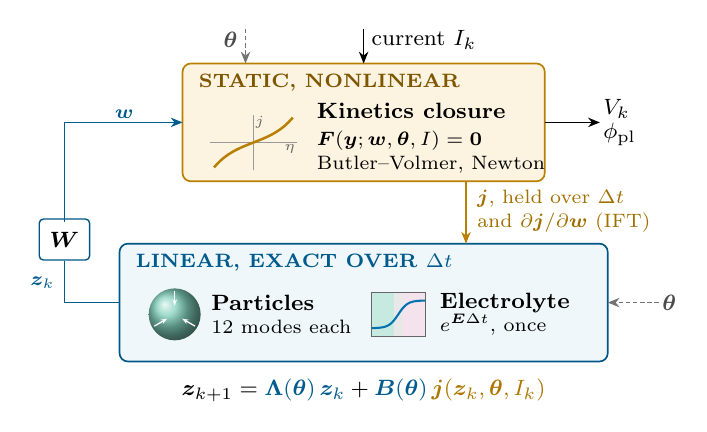
\begin{tikzpicture}[x=1mm, y=0.88mm, every node/.style={font=\footnotesize},
  arr/.style={-{Stealth[length=1.5mm, width=1.2mm]}, line width=0.55pt},
  lab/.style={font=\scriptsize, inner sep=1pt}]
% ---------- nonlinear block: kinetics closure ----------
\fill[cOra!12, rounded corners=3pt] (20,13) rectangle (66,30);
\draw[cOra!80!black, line width=0.6pt, rounded corners=3pt] (20,13) rectangle (66,30);
\node[anchor=north west, font=\scriptsize\bfseries, text=cOra!55!black, inner sep=0pt] at (22,28.6) {STATIC, NONLINEAR};
\begin{scope}[shift={(29,18.6)}]
  \draw[black!40, line width=0.3pt] (-5.5,0) -- (5.5,0) (0,-4) -- (0,4);
  \draw[cOra!80!black, line width=0.9pt] plot[smooth, domain=-5:5, samples=40] (\x,{3.6*sinh(0.36*\x)/sinh(0.36*5)});
  \node[font=\tiny, text=black!60, anchor=north east, inner sep=0.4pt] at (5.5,0) {$\eta$};
  \node[font=\tiny, text=black!60, anchor=north west, inner sep=0.4pt] at (0,4) {$j$};
\end{scope}
\node[anchor=west, align=left, inner sep=0pt] at (37,19.2) {\textbf{Kinetics closure}\\[0.2pt]{\scriptsize $\vF(\vy;\vw,\vth,I)=\bm 0$}\\[-0.6pt]{\scriptsize Butler--Volmer, Newton}};
% ---------- linear block: exact dynamics ----------
\fill[cBlu!6, rounded corners=3pt] (12,-13) rectangle (74,4);
\draw[cBlu!75!black, line width=0.6pt, rounded corners=3pt] (12,-13) rectangle (74,4);
\node[anchor=north west, font=\scriptsize\bfseries, text=cBlu!80!black, inner sep=0pt] at (14,2.6) {LINEAR, EXACT OVER $\Delta t$};
% particle icon
\shade[ball color=cGre!50] (19,-6.2) circle[radius=3.3mm];
\foreach \a in {90,210,330}{\draw[-{Stealth[length=0.8mm]}, white, line width=0.45pt] ([shift={(\a:3.0mm)}]19,-6.2) -- ([shift={(\a:1.1mm)}]19,-6.2);}
\node[anchor=west, align=left, inner sep=0pt] at (23.6,-6.2) {\textbf{Particles}\\[-1pt]{\scriptsize 12 modes each}};
% electrolyte icon
\begin{scope}[shift={(44,-9.4)}]
  \fill[cGre!22] (0,0) rectangle (2.8,6.4); \fill[black!9] (2.8,0) rectangle (4.0,6.4); \fill[cPur!22] (4.0,0) rectangle (6.8,6.4);
  \draw[black!60, line width=0.3pt] (0,0) rectangle (6.8,6.4);
  \draw[cBlu, line width=0.75pt] plot[smooth, domain=0:6.8] (\x,{3.2+2.0*tanh(0.85*(\x-3.4))});
\end{scope}
\node[anchor=west, align=left, inner sep=0pt] at (52.6,-6.2) {\textbf{Electrolyte}\\[-1pt]{\scriptsize $e^{\bm E\Delta t}$, once}};
% ---------- loop ----------
% state -> selector W -> w
\draw[line width=0.55pt, cBlu!80!black] (12,-4.5) -- (5,-4.5) -- (5,1.5);
\node[draw=cBlu!75!black, fill=white, line width=0.5pt, rounded corners=1.5pt, minimum width=6.4mm, minimum height=5.2mm, inner sep=0pt] (W) at (5,4.6) {$\bm W$};
\draw[arr, cBlu!80!black] (5,7.2) -- (5,21.5) -- (20,21.5);
\node[lab, text=cBlu!80!black, anchor=east] at (4.2,-1.6) {$\vz_k$};
\node[lab, text=cBlu!80!black, anchor=south, align=center] at (12.6,21.6) {$\vw$};
% j down into the linear block
\draw[arr, cOra!80!black] (56,13) -- (56,4);
\node[lab, text=cOra!70!black, anchor=west] at (57,10.5) {$\vj$, held over $\Delta t$};
\node[lab, text=cOra!70!black, anchor=west] at (57,7.1) {and $\partial\vj/\partial\vw$ (IFT)};
% inputs and outputs
\draw[arr] (43,35) -- (43,30); \node[anchor=west, inner sep=1pt] at (43.6,33.4) {current $I_k$};
\draw[arr] (66,21.5) -- (73,21.5) node[right, align=left, inner sep=1pt] {$V_k$\\[-1pt]$\phipl$};
\draw[arr, black!55, dash pattern=on 1.6pt off 1pt] (80.5,-4.5) node[right, text=black!70, inner sep=1pt] {$\vth$} -- (74,-4.5);
\draw[arr, black!55, dash pattern=on 1.6pt off 1pt] (28,35) -- (28,30); \node[anchor=east, text=black!70, inner sep=1pt] at (27.4,33.4) {$\vth$};
% ---------- the step ----------
\node[anchor=north, inner sep=1pt] at (43,-15) {$\vz_{k+1}=\textcolor{cBlu!80!black}{\mLam(\vth)\,\vz_k}+\textcolor{cBlu!80!black}{\mB(\vth)}\,\textcolor{cOra!75!black}{\vj(\vz_k,\vth,I_k)}$};
\end{tikzpicture}

\caption{The grey-box DFN as a loop. The linear dynamics (blue) are advanced exactly over each sampling interval; $\bm W$ reads the surface and electrolyte concentrations $\bm w$ from the state; the kinetics closure (orange), the only nonlinearity, gives the reaction currents $\bm j$, held over the next interval, the voltage and the plating potential, and $\partial\bm j/\partial\bm w$ by the implicit function theorem. Bottom: the step \eqref{eq:step}, same colours.}
\label{fig:scheme}
\end{figure}

This split makes the model both fast and easy to differentiate. If the reaction currents are held constant over a sampling interval $\Delta t$ (a zero-order hold, the only approximation in time), both linear parts can be advanced exactly, with no time-stepping error: each particle through its mean concentration and 12 exponentially decaying modes, plus a small correction for the faster modes we drop; the electrolyte, discretized in finite volumes as $\dot{\ce}=\bm E\ce+\bm G\vj$, through a matrix exponential computed once (Appendix~\ref{app:model}). Collecting these quantities in the state $\vz$, one step reads
\begin{equation}
\vz^{+}=\mLam(\vth)\,\vz+\mB(\vth)\,\vj(\vz,\vth,I),
\label{eq:step}
\end{equation}
where $\vth$ are the ageing parameters, $I$ is the applied current, $\mLam$ is block diagonal and $\mB$ maps the reaction currents into the state.

The reaction currents $\vj$, one per electrode cell, come from the \emph{kinetics closure} $\vF(\vy;\vw,\vth,I)=\bm 0$: 130 algebraic equations on the grid of Section~\ref{sec:grid}, solved by Newton's method at every step, whose unknowns $\vy$ are the reaction current and the electrolyte and solid potentials in each cell, and whose inputs $\vw$ are the surface and electrolyte concentrations read from $\vz$. Its solution also gives the voltage and the plating potential (Appendix~\ref{app:model}). We call this reorganized model the \emph{grey-box DFN}, and the EKF built on it the \emph{grey-box EKF}.

\subsection{The Derivative of the Step}\label{sec:ift}
A Kalman filter propagates its uncertainty with the Jacobian $\mA=\partial\vz^{+}/\partial\vz$, which says how the next state changes when the current one changes slightly, and learns the parameters through $\partial\vz^{+}/\partial\vth$. Differentiating \eqref{eq:step} gives
\begin{equation}
\mA=\mLam+\mB\,\mC,\qquad \mC=\frac{\partial\vj}{\partial\vz}=\frac{\partial\vj}{\partial\vw}\,\frac{\partial\vw}{\partial\vz}.
\label{eq:A}
\end{equation}
The first term, $\mLam$, is known. The second term, $\mB\mC$, says how the reaction currents respond to the state: $\mB$ is the known input matrix of the linear part and $\mC$ the response of the currents. The kinetics read only the concentrations $\vw$, so $\mC$ splits into two factors. $\partial\vw/\partial\vz$ is a fixed sparse matrix (a surface concentration, for instance, is the particle mean plus the modes evaluated at the surface). $\partial\vj/\partial\vw$ is the hard one: the currents are not an explicit formula of $\vw$ but the solution of $\vF(\vy;\vw)=\bm 0$, found by Newton's method. Yet this equation holds for every input: when $\vw$ changes, the solution $\vy$ moves so that $\vF$ stays zero. Differentiating this identity, $(\partial\vF/\partial\vy)(\partial\vy/\partial\vw)+\partial\vF/\partial\vw=\bm 0$, gives the implicit function theorem,
\begin{equation}
\frac{\partial\vy}{\partial\vw}=-\Big(\frac{\partial\vF}{\partial\vy}\Big)^{-1}\frac{\partial\vF}{\partial\vw},
\label{eq:ift}
\end{equation}
whose rows for the reaction currents are the missing factor in \eqref{eq:A}. In a scalar example, $F=y^3+y-w=0$ has no explicit solution $y(w)$, but \eqref{eq:ift} gives $\dd y/\dd w=1/(3y^2+1)$, that is $1/4$ at $w=2$, $y=1$. Replacing $\partial\vF/\partial\vw$ with $\partial\vF/\partial\vth$ gives in the same way the sensitivity to the ageing parameters.

In short, the derivative comes almost for free from the Newton solve the model performs anyway. The matrix $\partial\vF/\partial\vy$ is the one Newton has just factorized, so \eqref{eq:ift} costs a few triangular solves; and it is the derivative of the \emph{solution}, not of the procedure, so it does not depend on how many Newton iterations were taken or how they were started. The resulting $\mA$ agrees with automatic differentiation through the converged solver to $6\times10^{-13}$ in relative norm and costs \SI{0.5}{\milli\second} instead of \SI{122}{\milli\second} (Appendix~\ref{app:filter}). Because \eqref{eq:A} is a block-diagonal matrix plus a correction of rank $n_j$ (the number of electrode cells), the covariance prediction can also be formed blockwise, in $O(N^2n_j)$ instead of $O(N^3)$ operations. The model and all its derivatives then take only \SI{8}{\percent} of a filter step (Appendix~\ref{app:filter}); the rest is the dense covariance update.

\subsection{Filter and Spatial Grid}\label{sec:grid}
The filter is a standard EKF on the state $\vz$ augmented with the ageing parameters, which follow a random walk and are estimated in logit coordinates, a change of variable that keeps each within its physical range. The voltage noise is $\sigma_V=\SI{2}{\milli\volt}$ and the sampling interval $\Delta t=\SI{0.5}{\second}$. The initial cell state is known and the parameters start far from the truth; an unknown one would change little (Section~\ref{sec:ageing}). A state guard, a simple form of constrained filtering\cite{simon2010}, rejects any correction that would push a concentration outside its physical limits. Three parameters ($\Rf$, $\LAM$, $\Ds$) are estimated in Sections~\ref{sec:ageing}--\ref{sec:charge}, with $\LLI$ fixed; all four in Section~\ref{sec:tracking} (details in Appendix~\ref{app:filter}).

One choice mattered more than expected: where the grid cells are placed (Fig.~\ref{fig:grid}, mid-aged cell th2 of Section~\ref{sec:results}). With 20 cells per electrode and 10 in the separator, evenly spaced, the voltage error is only \SI{1.6}{\milli\volt} at 3C, yet fitting the parameters to noise-free reference data biases $\Ds$ by \SI{4.9}{\percent} of its range: the filter absorbs a small voltage error into the parameter to which the voltage is least sensitive. The bias comes from the grid, not from the particle model. On the coarsest grid, 12 modes instead of 8 change it only from 9.2 to 8.6\,\%, while each doubling of the uniform grid halves it (9.2, 4.9, 2.6\,\%), at a cost that grows from 1.3 to \SI{55}{\milli\second} per step. Shrinking the cells towards the separator, where plating starts, in a 4:1 geometric progression (negative-electrode cells from 7.8 to \SI{2.0}{\micro\metre}) reduces the voltage error to \SI{0.6}{\milli\volt} and the $\Ds$ bias to 1.3\,\%, with the same number of cells and the same cost as the uniform 20/10/20 grid: less bias than doubling the grid, at one seventh of its cost. This grid, with $N=653$ states including the parameters (654 when $\LLI$ is also estimated), is used throughout.
\begin{figure}[t]
\centering
% Effect of the spatial grid; value labels written from data/grid.csv. Data: data/grid.csv (mid-aged cell th2, M17; Table I merged into this figure)
\begin{tikzpicture}
\begin{groupplot}[paper, group style={group size=1 by 3, vertical sep=5mm, group name=g, x descriptions at=edge bottom},
  width=64mm, height=20mm, y label style={at={(axis description cs:-0.09,0.5)}, anchor=south}, xmin=-0.6, xmax=4.6, xtick={0,1,2,3,4},
  xticklabels={{10/5/10\\unif., 8\\248}, {10/5/10\\unif., 12\\328}, {20/10/20\\unif., 12\\653}, {40/20/40\\unif., 16\\1623}, {\textbf{20/10/20}\\\textbf{4:1, 12}\\\textbf{653}}},
  x tick label style={align=center, font=\scriptsize},
  xlabel={grid (cells), modes; number of states $N$}, /pgf/bar width=5pt,
  legend style={at={(0.98,0.97)}, anchor=north east, fill=none}, legend columns=3,
  legend style={/tikz/every even column/.append style={column sep=1.5mm}}]
\nextgroupplot[ymin=0, ymax=4.8, ytick={0,1,2,3,4}, ylabel={$E_V$ RMS (mV)}]
\addplot[ybar, bar shift=-3pt, fill=cSPMe, draw=none, barleg] table[x=x, y=panel_a_E_V_1C_mV, col sep=comma] {figures/data/grid.csv};
\addplot[ybar, bar shift=3pt, fill=cGB, draw=none, barleg, postaction={pattern=north east lines, pattern color=white}] table[x=x, y=panel_a_E_V_3C_mV, col sep=comma] {figures/data/grid.csv};
\legend{1C, 3C (30 s)}
\node[font=\tiny, inner sep=0.8pt, xshift=-3pt, rotate=90, anchor=west] at (axis cs:0,2.3041) {2.3};
\node[font=\tiny, inner sep=0.8pt, xshift=-3pt, rotate=90, anchor=west] at (axis cs:1,2.3045) {2.3};
\node[font=\tiny, inner sep=0.8pt, xshift=-3pt, rotate=90, anchor=west] at (axis cs:2,1.0668) {1.1};
\node[font=\tiny, inner sep=0.8pt, xshift=-3pt, rotate=90, anchor=west] at (axis cs:3,0.3975) {0.4};
\node[font=\tiny, inner sep=0.8pt, xshift=-3pt, rotate=90, anchor=west] at (axis cs:4,0.0309) {0.0};
\node[font=\tiny, inner sep=0.8pt, xshift=3pt, rotate=90, anchor=west] at (axis cs:0,3.5377) {3.5};
\node[font=\tiny, inner sep=0.8pt, xshift=3pt, rotate=90, anchor=west] at (axis cs:1,3.6632) {3.7};
\node[font=\tiny, inner sep=0.8pt, xshift=3pt, rotate=90, anchor=west] at (axis cs:2,1.5506) {1.6};
\node[font=\tiny, inner sep=0.8pt, xshift=3pt, rotate=90, anchor=west] at (axis cs:3,0.4915) {0.5};
\node[font=\tiny, inner sep=0.8pt, xshift=3pt, rotate=90, anchor=west] at (axis cs:4,0.6002) {0.6};
\nextgroupplot[ymin=0, ymax=13.5, ytick={0,4,8,12}, ylabel={$|$bias$|$ (\% of range)}]
\addplot[ybar, bar shift=-5.5pt, fill=cGre, draw=none, barleg] table[x=x, y=panel_b_abs_bias_Rf_pct_of_range, col sep=comma] {figures/data/grid.csv};
\addplot[ybar, bar shift=0pt, fill=cBlu, draw=none, barleg, postaction={pattern=crosshatch dots, pattern color=white}] table[x=x, y=panel_b_abs_bias_LAM_pct_of_range, col sep=comma] {figures/data/grid.csv};
\addplot[ybar, bar shift=5.5pt, fill=cPur, draw=none, barleg, postaction={pattern=north east lines, pattern color=white}] table[x=x, y=panel_b_abs_bias_Ds_pct_of_range, col sep=comma] {figures/data/grid.csv};
\legend{$R_{\mathrm{f}}$, LAM, $D_{\mathrm{s}}$}
\node[font=\tiny, inner sep=0.8pt, xshift=-5.5pt, rotate=90, anchor=west] at (axis cs:0,6.0773) {6.1};
\node[font=\tiny, inner sep=0.8pt, xshift=-5.5pt, rotate=90, anchor=west] at (axis cs:1,6.6249) {6.6};
\node[font=\tiny, inner sep=0.8pt, xshift=-5.5pt, rotate=90, anchor=west] at (axis cs:2,2.5903) {2.6};
\node[font=\tiny, inner sep=0.8pt, xshift=-5.5pt, rotate=90, anchor=west] at (axis cs:3,0.4373) {0.4};
\node[font=\tiny, inner sep=0.8pt, xshift=-5.5pt, rotate=90, anchor=west] at (axis cs:4,0.8967) {0.9};
\node[font=\tiny, inner sep=0.8pt, xshift=0pt, rotate=90, anchor=west] at (axis cs:0,0.5935) {0.6};
\node[font=\tiny, inner sep=0.8pt, xshift=0pt, rotate=90, anchor=west] at (axis cs:1,0.5497) {0.5};
\node[font=\tiny, inner sep=0.8pt, xshift=0pt, rotate=90, anchor=west] at (axis cs:2,0.3188) {0.3};
\node[font=\tiny, inner sep=0.8pt, xshift=0pt, rotate=90, anchor=west] at (axis cs:3,0.1767) {0.2};
\node[font=\tiny, inner sep=0.8pt, xshift=0pt, rotate=90, anchor=west] at (axis cs:4,0.1033) {0.1};
\node[font=\tiny, inner sep=0.8pt, xshift=5.5pt, rotate=90, anchor=west] at (axis cs:0,9.2066) {9.2};
\node[font=\tiny, inner sep=0.8pt, xshift=5.5pt, rotate=90, anchor=west] at (axis cs:1,8.6154) {8.6};
\node[font=\tiny, inner sep=0.8pt, xshift=5.5pt, rotate=90, anchor=west] at (axis cs:2,4.8878) {4.9};
\node[font=\tiny, inner sep=0.8pt, xshift=5.5pt, rotate=90, anchor=west] at (axis cs:3,2.5643) {2.6};
\node[font=\tiny, inner sep=0.8pt, xshift=5.5pt, rotate=90, anchor=west] at (axis cs:4,1.2624) {1.3};
\nextgroupplot[ymode=log, log origin=infty, ymin=0.5, ymax=300, ytick={1,10,100}, yticklabels={1,10,100}, ylabel={step cost (ms)}]
\addplot[ybar, bar shift=0pt, fill=cGB!70, draw=none] table[x=x, y=cost_ms, col sep=comma] {figures/data/grid.csv};
\node[font=\tiny, inner sep=0.8pt, anchor=south] at (axis cs:0,1.2996) {1.3};
\node[font=\tiny, inner sep=0.8pt, anchor=south] at (axis cs:1,1.8537) {1.9};
\node[font=\tiny, inner sep=0.8pt, anchor=south] at (axis cs:2,7.9039) {7.9};
\node[font=\tiny, inner sep=0.8pt, anchor=south] at (axis cs:3,54.8383) {55};
\node[font=\tiny, inner sep=0.8pt, anchor=south] at (axis cs:4,7.9370) {7.9};
\end{groupplot}
% panel (a): cell boundaries of the two 20/10/20 grids (Chen et al. thicknesses 85.2 / 12 / 75.6 um)
\begin{axis}[paper, name=grids, at={($(g c1r1.north west)+(0,13mm)$)}, anchor=south west, width=64mm, height=11mm, xmin=0, xmax=172.8, ymin=0, ymax=2,
  ytick={0.5,1.5}, yticklabels={4:1, uniform}, xtick={0,85.2,97.2,172.8}, xticklabels={0,85,97,173},
  xlabel={position across the cell ($\mu$m)}, axis line style={draw=none}, tick style={draw=none}, clip=false]
\fill[cGre!18] (axis cs:0,0) rectangle (axis cs:85.2,2);
\fill[black!6] (axis cs:85.2,0) rectangle (axis cs:97.2,2);
\fill[cPur!18] (axis cs:97.2,0) rectangle (axis cs:172.8,2);
\draw[line width=0.25pt] (axis cs:0.00,1.1) -- (axis cs:0.00,1.9) (axis cs:4.26,1.1) -- (axis cs:4.26,1.9) (axis cs:8.52,1.1) -- (axis cs:8.52,1.9) (axis cs:12.78,1.1) -- (axis cs:12.78,1.9) (axis cs:17.04,1.1) -- (axis cs:17.04,1.9) (axis cs:21.30,1.1) -- (axis cs:21.30,1.9) (axis cs:25.56,1.1) -- (axis cs:25.56,1.9) (axis cs:29.82,1.1) -- (axis cs:29.82,1.9) (axis cs:34.08,1.1) -- (axis cs:34.08,1.9) (axis cs:38.34,1.1) -- (axis cs:38.34,1.9) (axis cs:42.60,1.1) -- (axis cs:42.60,1.9) (axis cs:46.86,1.1) -- (axis cs:46.86,1.9) (axis cs:51.12,1.1) -- (axis cs:51.12,1.9) (axis cs:55.38,1.1) -- (axis cs:55.38,1.9) (axis cs:59.64,1.1) -- (axis cs:59.64,1.9) (axis cs:63.90,1.1) -- (axis cs:63.90,1.9) (axis cs:68.16,1.1) -- (axis cs:68.16,1.9) (axis cs:72.42,1.1) -- (axis cs:72.42,1.9) (axis cs:76.68,1.1) -- (axis cs:76.68,1.9) (axis cs:80.94,1.1) -- (axis cs:80.94,1.9) (axis cs:85.20,1.1) -- (axis cs:85.20,1.9) (axis cs:86.40,1.1) -- (axis cs:86.40,1.9) (axis cs:87.60,1.1) -- (axis cs:87.60,1.9) (axis cs:88.80,1.1) -- (axis cs:88.80,1.9) (axis cs:90.00,1.1) -- (axis cs:90.00,1.9) (axis cs:91.20,1.1) -- (axis cs:91.20,1.9) (axis cs:92.40,1.1) -- (axis cs:92.40,1.9) (axis cs:93.60,1.1) -- (axis cs:93.60,1.9) (axis cs:94.80,1.1) -- (axis cs:94.80,1.9) (axis cs:96.00,1.1) -- (axis cs:96.00,1.9) (axis cs:97.20,1.1) -- (axis cs:97.20,1.9) (axis cs:100.98,1.1) -- (axis cs:100.98,1.9) (axis cs:104.76,1.1) -- (axis cs:104.76,1.9) (axis cs:108.54,1.1) -- (axis cs:108.54,1.9) (axis cs:112.32,1.1) -- (axis cs:112.32,1.9) (axis cs:116.10,1.1) -- (axis cs:116.10,1.9) (axis cs:119.88,1.1) -- (axis cs:119.88,1.9) (axis cs:123.66,1.1) -- (axis cs:123.66,1.9) (axis cs:127.44,1.1) -- (axis cs:127.44,1.9) (axis cs:131.22,1.1) -- (axis cs:131.22,1.9) (axis cs:135.00,1.1) -- (axis cs:135.00,1.9) (axis cs:138.78,1.1) -- (axis cs:138.78,1.9) (axis cs:142.56,1.1) -- (axis cs:142.56,1.9) (axis cs:146.34,1.1) -- (axis cs:146.34,1.9) (axis cs:150.12,1.1) -- (axis cs:150.12,1.9) (axis cs:153.90,1.1) -- (axis cs:153.90,1.9) (axis cs:157.68,1.1) -- (axis cs:157.68,1.9) (axis cs:161.46,1.1) -- (axis cs:161.46,1.9) (axis cs:165.24,1.1) -- (axis cs:165.24,1.9) (axis cs:169.02,1.1) -- (axis cs:169.02,1.9) (axis cs:172.80,1.1) -- (axis cs:172.80,1.9);
\draw[line width=0.25pt] (axis cs:0.00,0.1) -- (axis cs:0.00,0.9) (axis cs:7.81,0.1) -- (axis cs:7.81,0.9) (axis cs:15.07,0.1) -- (axis cs:15.07,0.9) (axis cs:21.82,0.1) -- (axis cs:21.82,0.9) (axis cs:28.10,0.1) -- (axis cs:28.10,0.9) (axis cs:33.93,0.1) -- (axis cs:33.93,0.9) (axis cs:39.35,0.1) -- (axis cs:39.35,0.9) (axis cs:44.39,0.1) -- (axis cs:44.39,0.9) (axis cs:49.08,0.1) -- (axis cs:49.08,0.9) (axis cs:53.44,0.1) -- (axis cs:53.44,0.9) (axis cs:57.49,0.1) -- (axis cs:57.49,0.9) (axis cs:61.25,0.1) -- (axis cs:61.25,0.9) (axis cs:64.75,0.1) -- (axis cs:64.75,0.9) (axis cs:68.01,0.1) -- (axis cs:68.01,0.9) (axis cs:71.03,0.1) -- (axis cs:71.03,0.9) (axis cs:73.84,0.1) -- (axis cs:73.84,0.9) (axis cs:76.46,0.1) -- (axis cs:76.46,0.9) (axis cs:78.89,0.1) -- (axis cs:78.89,0.9) (axis cs:81.15,0.1) -- (axis cs:81.15,0.9) (axis cs:83.25,0.1) -- (axis cs:83.25,0.9) (axis cs:85.20,0.1) -- (axis cs:85.20,0.9) (axis cs:86.40,0.1) -- (axis cs:86.40,0.9) (axis cs:87.60,0.1) -- (axis cs:87.60,0.9) (axis cs:88.80,0.1) -- (axis cs:88.80,0.9) (axis cs:90.00,0.1) -- (axis cs:90.00,0.9) (axis cs:91.20,0.1) -- (axis cs:91.20,0.9) (axis cs:92.40,0.1) -- (axis cs:92.40,0.9) (axis cs:93.60,0.1) -- (axis cs:93.60,0.9) (axis cs:94.80,0.1) -- (axis cs:94.80,0.9) (axis cs:96.00,0.1) -- (axis cs:96.00,0.9) (axis cs:97.20,0.1) -- (axis cs:97.20,0.9) (axis cs:98.93,0.1) -- (axis cs:98.93,0.9) (axis cs:100.80,0.1) -- (axis cs:100.80,0.9) (axis cs:102.80,0.1) -- (axis cs:102.80,0.9) (axis cs:104.96,0.1) -- (axis cs:104.96,0.9) (axis cs:107.28,0.1) -- (axis cs:107.28,0.9) (axis cs:109.77,0.1) -- (axis cs:109.77,0.9) (axis cs:112.46,0.1) -- (axis cs:112.46,0.9) (axis cs:115.34,0.1) -- (axis cs:115.34,0.9) (axis cs:118.45,0.1) -- (axis cs:118.45,0.9) (axis cs:121.79,0.1) -- (axis cs:121.79,0.9) (axis cs:125.38,0.1) -- (axis cs:125.38,0.9) (axis cs:129.25,0.1) -- (axis cs:129.25,0.9) (axis cs:133.41,0.1) -- (axis cs:133.41,0.9) (axis cs:137.88,0.1) -- (axis cs:137.88,0.9) (axis cs:142.69,0.1) -- (axis cs:142.69,0.9) (axis cs:147.87,0.1) -- (axis cs:147.87,0.9) (axis cs:153.44,0.1) -- (axis cs:153.44,0.9) (axis cs:159.43,0.1) -- (axis cs:159.43,0.9) (axis cs:165.87,0.1) -- (axis cs:165.87,0.9) (axis cs:172.80,0.1) -- (axis cs:172.80,0.9);
\node[font=\scriptsize, anchor=south] at (axis cs:42.6,2) {negative};
\node[font=\scriptsize, anchor=south] at (axis cs:91.2,2) {sep.};
\node[font=\scriptsize, anchor=south] at (axis cs:135,2) {positive};
\end{axis}

\coordinate (L) at (current bounding box.west);
\foreach \p/\l in {grids/a, g c1r1/b, g c1r2/c, g c1r3/d}{\node[anchor=south west, font=\footnotesize, inner sep=0pt] at ($(L |- \p.north)+(0,1.2mm)$) {(\l)};}
\end{tikzpicture}

\caption{A non-uniform grid removes most of the model bias at no cost. (a) Cell boundaries across the cell for the uniform and the 4:1 grid, both with 20/10/20 cells (electrode thicknesses of the parameter set\cite{chen2020}): the 4:1 grid shrinks the electrode cells geometrically towards the separator, where plating starts, from 7.8 to \SI{2.0}{\micro\metre} in the negative electrode. (b) Closed-loop RMS voltage error against the reference at 1C and 3C (\SI{30}{\second}) for each grid, number of particle modes and number of states $N$; the last group is the 4:1 grid. (c) Absolute bias of a batch fit of the three ageing parameters to noise-free reference data; $\Ds$ is underestimated on every grid. (d) Cost of a full EKF step on one desktop core. All values for the mid-aged cell th2.}
\label{fig:grid}
\end{figure}


% ===================================================================
% ===================================================================
\section{Results}\label{sec:results}
All tests use the reference of Section~\ref{sec:model} as the truth. Five true ageing states $(\Rf,\LAM,\LLI,\Ds)$ are used: a fresh cell, th1 $(1,0,0,1)$; a mid-aged cell, th2 $(4,0.1,0.05,0.55)$; a cell at the corner of the range, th3 $(10,0.3,0.2,0.3)$; and two random draws, th4 $(8.51,0.179,0.058,0.330)$ and th5 $(9.49,0.108,0.157,0.714)$. Each test has two phases. The filter first learns the parameters on an estimation protocol (P6L, run twice: \SI{72}{\minute}) of $\pm$1C and $\pm$3C pulses, rests and slow discharges; its $-3$C pulses exceed \SI{4.2}{\volt}, so it is a test-bench protocol rather than BMS operation. It then continues, with what it has learned, on an evaluation protocol: a charge (F6Q: a 1C constant-current charge, then two 2C pulses that stop at \SI{4.2}{\volt}, as a BMS would) or a discharge with 1C, 2C and 3C pulses. For th3 the protocols start at a higher state of charge and its 1C charge is shorter (Appendix~\ref{app:protocols}). The analyses follow the order in which a BMS relies on the filter, each using what the previous one established: the filter must run fast enough (Section~\ref{sec:cost}), learn the ageing parameters of a cell of fixed age (Section~\ref{sec:ageing}), estimate with them the internal quantities that decide plating (Section~\ref{sec:charge}), and keep up as the cell ages (Section~\ref{sec:tracking}).
\subsection{Cost}\label{sec:cost}
One filter step takes \SI{7.9}{\milli\second} at $N=653$ on one desktop core (Fig.~\ref{fig:cost}), from \SI{0.64}{\milli\second} at $N=168$ to \SI{11.9}{\milli\second} at $N=813$, On a fixed grid the covariance propagation dominates and the cost grows as $N^2$; across Fig.~\ref{fig:cost} it grows more slowly, about as $N^{1.5}$, because $N$ is raised partly by adding cells, which enlarges the closure only linearly. An unscented Kalman filter (UKF) on the same model, which runs one Newton iteration of the kinetics at each of its $2N+1$ sigma points, takes \SI{287}{\milli\second}, 36 times more.

\begin{figure}[t]
\centering
% Cost of one filter step versus state dimension. Data: data/cost_*.csv
\begin{tikzpicture}
\begin{axis}[paper, width=60mm, height=32mm, xmode=log, ymode=log, xmin=150, xmax=950, ymin=0.4, ymax=500,
  xtick={200,300,400,600,800}, xticklabels={200,300,400,600,800}, minor xtick={}, 
  ytick={1,10,100}, yticklabels={1,10,100},
  xlabel={state dimension $N$}, ylabel={step cost (ms)}, legend style={at={(0.02,0.98)}, anchor=north west}]
\draw[cGrey, line width=0.3pt, dash pattern=on 1pt off 1pt] (axis cs:150,10) -- (axis cs:950,10);
\addplot[cGB, line width=0.8pt, mark=*, mark size=1.4pt] table[x=state_dimension_N, y=median_step_cost_ms, col sep=comma] {figures/data/cost_EKF.csv};
\addplot[only marks, cBlu, mark=diamond*, mark size=2pt] table[x=state_dimension_N, y=median_step_cost_ms, col sep=comma] {figures/data/cost_UKF_full.csv};
\legend{grey-box EKF, UKF on the same model}
\node[anchor=south west, font=\footnotesize, text=black!60] at (axis cs:155,10.5) {10 ms};
\node[anchor=north west, font=\tiny, inner sep=1pt, text=cGB!80!black] at (axis cs:168,0.638) {0.64};
\node[anchor=north west, font=\tiny, inner sep=1pt, text=cGB!80!black] at (axis cs:248,1.277) {1.28};
\node[anchor=north west, font=\tiny, inner sep=1pt, text=cGB!80!black] at (axis cs:328,1.813) {1.81};
\node[anchor=north west, font=\tiny, inner sep=1pt, text=cGB!80!black] at (axis cs:493,4.05) {4.05};
\node[anchor=north west, font=\tiny, inner sep=1pt, text=cGB!80!black] at (axis cs:653,7.94) {7.94};
\node[anchor=south east, font=\tiny, inner sep=1pt, text=cGB!80!black] at (axis cs:813,11.9) {11.9};
\node[anchor=east, font=\tiny, inner sep=1.5pt, text=cBlu!80!black] at (axis cs:653,287) {287};
\end{axis}
\end{tikzpicture}

\caption{Median cost of one filter step versus the number of states on one desktop core (JAX, Python dispatch); dotted: \SI{10}{\milli\second}. $N$ is varied through the 10/5/10 and 20/10/20 4:1 grids with 4 to 16 particle modes. UKF on the same grey-box model, with one Newton iteration of the kinetics at every sigma point (Table~\ref{tab:filters} in Appendix~\ref{app:filter}).}
\label{fig:cost}
\end{figure}


\subsection{Ageing Parameters of a Cell at a Given Age}\label{sec:ageing}
We first ask how well the filter recovers the ageing parameters of a cell whose age does not change. For each of the five states we ran the filter ten times over the estimation protocol, each time with its own noise sequence and from a wrong initial guess: the true values plus errors drawn uniformly within $\pm$\SI{40}{\percent} of each parameter's range (clipped to the range), with an initial standard deviation of \SI{30}{\percent} of the range (Appendix~\ref{app:filter}). Errors are absolute, in percent of each parameter's range (1\,\% is 0.09 for $\Rf$, 0.003 for $\LAM$): relative errors would be undefined at the fresh cell, where $\LAM$ and $\LLI$ are zero. Fig.~\ref{fig:mc} compares the final estimates with the true values: points on the diagonal are exact. The typical error (RMSE over the ten runs) is at most 1.1\,\% of the range at the four aged states and 2.6\,\% for $\Ds$ at the fresh cell (Fig.~\ref{fig:mc}d--f, blue bars).

An error figure alone mixes three causes, each with a different remedy: the data may not contain the information, the model may differ from the cell, or the filter may misjudge its own uncertainty. We separate them with three experiments.

\begin{figure*}[t]
\centering
% Static tests. Row 1: Monte Carlo estimates against the truth (data/mc_th*.csv). Row 2: error budget per state
% (data/mc_budget.csv: RMSE over 10 runs, |model bias|, Cramer-Rao bound; % of range).
\pgfplotsset{discard if not/.style 2 args={x filter/.append code={\edef\tempa{\thisrow{#1}}\edef\tempb{#2}\ifx\tempa\tempb\else\def\pgfmathresult{inf}\fi}}}
\pgfplotsset{mcth1/.style={only marks, mark=o, mark size=1.7pt, cOra, line width=0.5pt},
  mcth2/.style={only marks, mark=square, mark size=1.5pt, cSPMe, line width=0.5pt},
  mcth3/.style={only marks, mark=triangle, mark size=2pt, cGre, line width=0.5pt},
  mcth4/.style={only marks, mark=diamond, mark size=2pt, cPur, line width=0.5pt},
  mcth5/.style={only marks, mark=pentagon, mark size=1.8pt, cBlu, line width=0.5pt}}
\begin{tikzpicture}
\begin{groupplot}[paper, group style={group size=3 by 2, horizontal sep=13mm, vertical sep=11mm, group name=g}, width=40mm, height=25mm]
\nextgroupplot[xmin=0, xmax=11, ymin=0, ymax=11, xtick={0,5,10}, ytick={0,5,10},
  xlabel={true $R_{\mathrm{f}}$}, ylabel={estimated $R_{\mathrm{f}}$},
  legend style={at={(0.02,0.98)}, anchor=north west}]
\draw[cGrey, line width=0.3pt] (axis cs:0,0) -- (axis cs:11,11);
\addplot[mcth1] table[x=a_Rf_true_over_Rf0, y=a_Rf_estimated_over_Rf0, col sep=comma] {figures/data/mc_th1.csv};
\addplot[mcth2] table[x=a_Rf_true_over_Rf0, y=a_Rf_estimated_over_Rf0, col sep=comma] {figures/data/mc_th2.csv};
\addplot[mcth3] table[x=a_Rf_true_over_Rf0, y=a_Rf_estimated_over_Rf0, col sep=comma] {figures/data/mc_th3.csv};
\addplot[mcth4] table[x=a_Rf_true_over_Rf0, y=a_Rf_estimated_over_Rf0, col sep=comma] {figures/data/mc_th4.csv};
\addplot[mcth5] table[x=a_Rf_true_over_Rf0, y=a_Rf_estimated_over_Rf0, col sep=comma] {figures/data/mc_th5.csv};
\legend{th1, th2, th3, th4, th5}
\nextgroupplot[xmin=-0.02, xmax=0.32, ymin=-0.02, ymax=0.32, xtick={0,0.1,0.2,0.3}, ytick={0,0.1,0.2,0.3},
  xticklabel style={/pgf/number format/fixed}, yticklabel style={/pgf/number format/fixed},
  xlabel={true LAM}, ylabel={estimated LAM}]
\draw[cGrey, line width=0.3pt] (axis cs:-0.02,-0.02) -- (axis cs:0.32,0.32);
\addplot[mcth1] table[x=b_LAM_true, y=b_LAM_estimated, col sep=comma] {figures/data/mc_th1.csv};
\addplot[mcth2] table[x=b_LAM_true, y=b_LAM_estimated, col sep=comma] {figures/data/mc_th2.csv};
\addplot[mcth3] table[x=b_LAM_true, y=b_LAM_estimated, col sep=comma] {figures/data/mc_th3.csv};
\addplot[mcth4] table[x=b_LAM_true, y=b_LAM_estimated, col sep=comma] {figures/data/mc_th4.csv};
\addplot[mcth5] table[x=b_LAM_true, y=b_LAM_estimated, col sep=comma] {figures/data/mc_th5.csv};
\nextgroupplot[xmin=0.2, xmax=1.1, ymin=0.2, ymax=1.1, xtick={0.2,0.6,1}, ytick={0.2,0.6,1},
  xticklabel style={/pgf/number format/fixed}, yticklabel style={/pgf/number format/fixed},
  xlabel={true $D_{\mathrm{s}}$}, ylabel={estimated $D_{\mathrm{s}}$}]
\draw[cGrey, line width=0.3pt] (axis cs:0.2,0.2) -- (axis cs:1.1,1.1);
\addplot[mcth1] table[x=c_Ds_true_over_Ds0, y=c_Ds_estimated_over_Ds0, col sep=comma] {figures/data/mc_th1.csv};
\addplot[mcth2] table[x=c_Ds_true_over_Ds0, y=c_Ds_estimated_over_Ds0, col sep=comma] {figures/data/mc_th2.csv};
\addplot[mcth3] table[x=c_Ds_true_over_Ds0, y=c_Ds_estimated_over_Ds0, col sep=comma] {figures/data/mc_th3.csv};
\addplot[mcth4] table[x=c_Ds_true_over_Ds0, y=c_Ds_estimated_over_Ds0, col sep=comma] {figures/data/mc_th4.csv};
\addplot[mcth5] table[x=c_Ds_true_over_Ds0, y=c_Ds_estimated_over_Ds0, col sep=comma] {figures/data/mc_th5.csv};
\nextgroupplot[height=14mm, xmin=-0.6, xmax=4.6, ymin=0, ymax=1.5, ytick={0,0.5,1}, xtick={0,1,2,3,4}, xticklabels={th1,th2,th3,th4,th5}, /pgf/bar width=3.6pt, ylabel={\% of range}]
\addplot[ybar, bar shift=-4pt, fill=cBlu, draw=none, discard if not={param}{Rf}] table[x=x, y=rmse, col sep=comma] {figures/data/mc_budget.csv};
\addplot[ybar, bar shift=0pt, fill=cOra, draw=none, postaction={pattern=north east lines, pattern color=white}, discard if not={param}{Rf}] table[x=x, y=abs_bias, col sep=comma] {figures/data/mc_budget.csv};
\addplot[ybar, bar shift=4pt, fill=cGrey!70, draw=none, discard if not={param}{Rf}] table[x=x, y=crlb, col sep=comma] {figures/data/mc_budget.csv};
\nextgroupplot[height=14mm, xmin=-0.6, xmax=4.6, ymin=0, ymax=0.6, ytick={0,0.2,0.4}, xtick={0,1,2,3,4}, xticklabels={th1,th2,th3,th4,th5}, /pgf/bar width=3.6pt]
\addplot[ybar, bar shift=-4pt, fill=cBlu, draw=none, discard if not={param}{LAM}] table[x=x, y=rmse, col sep=comma] {figures/data/mc_budget.csv};
\addplot[ybar, bar shift=0pt, fill=cOra, draw=none, postaction={pattern=north east lines, pattern color=white}, discard if not={param}{LAM}] table[x=x, y=abs_bias, col sep=comma] {figures/data/mc_budget.csv};
\addplot[ybar, bar shift=4pt, fill=cGrey!70, draw=none, discard if not={param}{LAM}] table[x=x, y=crlb, col sep=comma] {figures/data/mc_budget.csv};
\nextgroupplot[height=14mm, xmin=-0.6, xmax=4.6, ymin=0, ymax=3, ytick={0,1,2,3}, xtick={0,1,2,3,4}, xticklabels={th1,th2,th3,th4,th5}, /pgf/bar width=3.6pt]
\addplot[ybar, bar shift=-4pt, fill=cBlu, draw=none, discard if not={param}{Ds}] table[x=x, y=rmse, col sep=comma] {figures/data/mc_budget.csv};
\addplot[ybar, bar shift=0pt, fill=cOra, draw=none, postaction={pattern=north east lines, pattern color=white}, discard if not={param}{Ds}] table[x=x, y=abs_bias, col sep=comma] {figures/data/mc_budget.csv};
\addplot[ybar, bar shift=4pt, fill=cGrey!70, draw=none, discard if not={param}{Ds}] table[x=x, y=crlb, col sep=comma] {figures/data/mc_budget.csv};
\end{groupplot}
\plab{g c1r1}{a}\plab{g c2r1}{b}\plab{g c3r1}{c}\plab{g c1r2}{d}\plab{g c2r2}{e}\plab{g c3r2}{f}
\end{tikzpicture}

\caption{Static tests. (a)--(c) Ageing parameters estimated from voltage against their true values at the end of the estimation protocol: film resistance, loss of active material, diffusivity. Five true states, ten runs each with random initial errors and noise; on the diagonal the estimate is exact. (d)--(f) Where the error comes from, in \% of each parameter's range. Blue: error of our filter (RMSE over the ten runs). Orange, hatched: error of a perfect filter on our model (model bias). Grey: best precision these data allow (Cram\'er--Rao bound, with $\LLI$ fixed as in the filter). Blue close to orange: the error comes from the model, not from the filter.}
\label{fig:mc}
\end{figure*}

\begin{figure}[t]
\centering
% Consistency in the twin experiment: histogram of the time-averaged NEES per run. Data: data/nees_*.csv, nees_means.csv
\begin{tikzpicture}
\begin{groupplot}[paper, group style={group size=2 by 1, horizontal sep=7mm, group name=g, y descriptions at=edge left},
  width=29mm, height=26mm, xmin=0, xmax=10, ymin=0, ymax=12, xtick={0,2,...,10}, xticklabels={0,2,4,6,8,${\geq}10$},
  xlabel={NEES per run}, /pgf/bar width=2.6pt, legend style={at={(0.98,0.98)}, anchor=north east, fill=none}]
\nextgroupplot[ylabel={runs}]
\fill[black!8] (axis cs:1,0) rectangle (axis cs:3,12);
\addplot[ybar, bar shift=-1.3pt, fill=cGB, draw=none, barleg] table[x=x, y=n, col sep=comma] {figures/data/nees_a_EKF.csv};
\addplot[ybar, bar shift=1.3pt, fill=cSPMe, draw=none, barleg, postaction={pattern=north east lines, pattern color=white}] table[x=x, y=n, col sep=comma] {figures/data/nees_a_UKF.csv};
\legend{EKF (2.21), UKF (11.2)}
\nextgroupplot
\fill[black!8] (axis cs:1,0) rectangle (axis cs:3,12);
\addplot[ybar, fill=cGB, draw=none, barleg] table[x=x, y=n, col sep=comma] {figures/data/nees_b_EKF.csv};
\legend{EKF (15.0)}
\end{groupplot}
\node[anchor=south west, font=\footnotesize, inner sep=0pt] at ($(g c1r1.north west)+(0,1.4mm)$) {(a) th2, mid-aged};
\node[anchor=south west, font=\footnotesize, inner sep=0pt] at ($(g c2r1.north west)+(0,1.4mm)$) {(b) th1, fresh};
\end{tikzpicture}

\caption{Is the filter honest about its uncertainty? Time-averaged NEES of $(\Rf,\Ds)$ in each twin run (expected 2); the band $[1,3]$ applies to the mean over runs, in parentheses. (a) Mid-aged cell th2: EKF and UKF with the same tuning, 20 runs each. (b) Fresh cell th1: EKF, 20 runs.}
\label{fig:nees}
\end{figure}

\emph{Do the data contain the information?} The Cram\'er--Rao bound is the smallest standard deviation that any unbiased method could reach from these data and this noise, computed from the Fisher information $\mathcal I=\sigma_V^{-2}\sum_k(\mathrm{d}V_k/\mathrm{d}\vth)^{\top}(\mathrm{d}V_k/\mathrm{d}\vth)$, with the total sensitivities propagated along the trajectory by the exact derivatives of Section~\ref{sec:model}, for the three estimated parameters with $\LLI$ fixed as in the filter (grey bars in Fig.~\ref{fig:mc}d--f). They stay at or below 0.55\,\% of the range, except for $\Ds$ at the fresh cell (1.6\,\%), whose voltage depends least on diffusion. An unknown initial state of charge raises the bound for $\LAM$, which it mimics, to 0.5\,\% at most, and moves the others by 0.12\,\% at most. The data are informative, except for one pair: on pulses, $\LAM$ and $\LLI$ change the voltage almost alike (correlation 0.89--0.98), so only one can be estimated; we fix $\LLI$.

\emph{Is the error the filter's or the model's?} We fit the parameters to noise-free reference data by Gauss--Newton, as a perfect filter would; the error that remains belongs to the model (orange bars in Fig.~\ref{fig:mc}d--f). Our filter's error is close to it. Removing it leaves at most 0.3\,\% of the range at the aged states (0.7\,\% for $\Ds$ at th2): most of the error belongs to the model, not to the filter.

\emph{Does the filter know how uncertain it is?} With each estimate the filter reports a covariance $\mP_\theta$, an error bar. In a \emph{twin} experiment the data come from the filter's own model plus noise, so the model is exact and any problem is the filter's. The normalized estimation error squared (NEES)\cite{barshalom2001}, $\epsilon=\tilde{\vth}^{\top}\mP_{\theta}^{-1}\tilde{\vth}$ with $\tilde{\vth}$ the error, measures the error in units of the reported bar and should average the number of parameters. We compute it on $(\Rf,\Ds)$ in logit coordinates, average it over time in each run and accept a mean over at least 20 runs in $[1,3]$ (expected 2); adding $\LAM$ does not change the verdicts (Appendix~\ref{app:filter}). At the mid-aged cell it is 2.2 (Fig.~\ref{fig:nees}), inside the band. An unscented filter on the same model and tuning does not pass (mean 11.2, five runs above 10), although its errors against the reference are similar to the EKF's (Table~\ref{tab:filters} in Appendix~\ref{app:filter}). At the fresh cell the NEES is 15. In six of 20 runs the film resistance, started several times too high, was approached slowly while the filter already reported a narrow error bar. The errors remain small (at most 2.1\,\% for $\Rf$), but at this corner of the range, where all three parameters sit at the edge, the reported uncertainty is too optimistic (Appendix~\ref{app:results}).

\subsection{Seeing Plating Coming During Charge}\label{sec:charge}
With the parameters it has learned, the filter continues on the charge protocol. The quantities that matter there are evaluated at the boundary between the negative electrode and the separator, where plating starts: the reaction overpotential $\eta$ and the plating potential
\begin{equation}
\phipl=\phi_{\mathrm s}-\phi_{\mathrm e}-\Rf R^{0}_{\mathrm f}\,j,
\label{eq:phipl}
\end{equation}
the potential of the solid ($\phi_{\mathrm s}$) against the electrolyte ($\phi_{\mathrm e}$), corrected for the drop across the film carried by the reaction current $j$ of that cell (its entry of the vector $\vj$ in \eqref{eq:step}), with $\Rf R^{0}_{\mathrm f}$ the film resistance. Plating is thermodynamically possible where $\phipl<0$\cite{arora1999}. The reference has no plating reaction: the zero crossing is an event to detect, not a prediction of plated lithium. We report the RMS error of $\phipl$ and $\eta$ and how late the estimate crosses \SI{0}{\milli\volt} after the reference (the early-warning thresholds $+20$ and $+10$\,mV are in Appendix~\ref{app:results}). A positive error of $\phipl$ places the cell farther from plating than it is: it is the unsafe side.

The current-practice baseline is an unscented Kalman filter on the SPMe that estimates the same three parameters with the same noise settings and initialization; its plating potential is the one the SPMe predicts at the separator from its single negative particle (Appendix~\ref{app:filter}).

Fig.~\ref{fig:charge}a--c shows the plating potential at the separator during the first 2C charge pulse. In the reference it drops below zero within the first second of every pulse and reaches $-23$ to \SI{-69}{\milli\volt} across the five states. Over both pulses and all states, the grey-box filter follows it within \SIrange{0.04}{0.56}{\milli\volt} RMS; the SPMe filter errs by \SIrange{4.1}{23.8}{\milli\volt}, 25 to 500 times more (Table~\ref{tab:pulse}; medians over ten runs). The reaction overpotential and the minimum electrolyte concentration, which limits the power the cell can deliver, show the same pattern (Table~\ref{tab:charge} in Appendix~\ref{app:results}). The SPMe error is mostly on the safe side, predicting the cell closer to plating than it is, which costs charging time; in the first pulse of th2, however, a median of 31\,\% of its samples were more than \SI{5}{\milli\volt} on the unsafe side (up to 65\,\% in single runs).

\begin{figure*}[t]
\centering
% Plating potential at the separator during charge. Data: data/pulse_th*.csv, data/cc_th*.csv, data/cc_crossings.csv
\begin{tikzpicture}
\begin{groupplot}[paper,
  group style={group size=3 by 2, horizontal sep=7mm, vertical sep=13mm, group name=g},
  width=50mm, height=29mm]
% ---------- row 1: first 2C charge pulse ----------
\nextgroupplot[xmin=-10, xmax=60, ymin=-110, ymax=140, ytick={-100,-50,0,50,100},
  xlabel={time from pulse start (s)}, ylabel={$\phi_{\mathrm{pl}}$ (mV)},
  legend to name=legcharge, legend columns=3, legend style={/tikz/every even column/.append style={column sep=6mm}}]
\fill[red!6] (axis cs:-10,-110) rectangle (axis cs:60,0);\draw[zero] (axis cs:-10,0) -- (axis cs:60,0);
\draw[cGrey, line width=0.3pt] (axis cs:30,-110) -- (axis cs:30,140);
\addplot[lref] table[x=t, y=phi_pl_reference_mV, col sep=comma] {figures/data/pulse_th1.csv};
\addplot[lgb] table[x=t, y=phi_pl_EKF_mV, col sep=comma] {figures/data/pulse_th1.csv};
\addplot[lspme] table[x=t, y=phi_pl_UKF_SPMe_mV, col sep=comma] {figures/data/pulse_th1.csv};
\legend{reference, grey-box EKF, SPMe UKF}
\node[anchor=south west, font=\footnotesize] at (rel axis cs:0.02,0.02) {th1, fresh};
\nextgroupplot[xmin=-10, xmax=60, ymin=-110, ymax=140, ytick={-100,-50,0,50,100}, yticklabels={},
  xlabel={time from pulse start (s)}]
\fill[red!6] (axis cs:-10,-110) rectangle (axis cs:60,0);\draw[zero] (axis cs:-10,0) -- (axis cs:60,0);
\draw[cGrey, line width=0.3pt] (axis cs:29,-110) -- (axis cs:29,140);
\addplot[lref] table[x=t, y=phi_pl_reference_mV, col sep=comma] {figures/data/pulse_th2.csv};
\addplot[lgb] table[x=t, y=phi_pl_EKF_mV, col sep=comma] {figures/data/pulse_th2.csv};
\addplot[lspme] table[x=t, y=phi_pl_UKF_SPMe_mV, col sep=comma] {figures/data/pulse_th2.csv};
\node[anchor=south west, font=\footnotesize] at (rel axis cs:0.02,0.02) {th2, mid-aged};
\nextgroupplot[xmin=-10, xmax=60, ymin=-110, ymax=140, ytick={-100,-50,0,50,100}, yticklabels={},
  xlabel={time from pulse start (s)}]
\fill[red!6] (axis cs:-10,-110) rectangle (axis cs:60,0);\draw[zero] (axis cs:-10,0) -- (axis cs:60,0);
\draw[cGrey, line width=0.3pt] (axis cs:21.5,-110) -- (axis cs:21.5,140);
\addplot[lref] table[x=t, y=phi_pl_reference_mV, col sep=comma] {figures/data/pulse_th4.csv};
\addplot[lgb] table[x=t, y=phi_pl_EKF_mV, col sep=comma] {figures/data/pulse_th4.csv};
\addplot[lspme] table[x=t, y=phi_pl_UKF_SPMe_mV, col sep=comma] {figures/data/pulse_th4.csv};
\node[anchor=south west, font=\footnotesize] at (rel axis cs:0.02,0.02) {th4, aged};
% ---------- row 2: 1C constant-current charge; markers at the first zero crossing ----------
\nextgroupplot[xmin=0, xmax=21.5, ymin=-25, ymax=60, xtick={0,5,10,15,20},
  xlabel={time from start of 1C charge (min)}, ylabel={$\phi_{\mathrm{pl}}$ (mV)}]
\fill[red!6] (axis cs:0,-25) rectangle (axis cs:21.5,0);\draw[zero] (axis cs:0,0) -- (axis cs:21.5,0);
\addplot[lref, forget plot] table[x=tmin, y=phi_pl_reference_mV, col sep=comma] {figures/data/cc_th1.csv};
\addplot[lgb, forget plot] table[x=tmin, y=phi_pl_EKF_mV, col sep=comma] {figures/data/cc_th1.csv};
\addplot[lspme, forget plot] table[x=tmin, y=phi_pl_UKF_SPMe_mV, col sep=comma] {figures/data/cc_th1.csv};
\node[anchor=south west, font=\footnotesize, text=red!55!black] at (axis cs:0.4,-24) {plating possible ($\phi_{\mathrm{pl}}<0$)};
\addplot[only marks, mark=o, mark size=2.2pt, cRef, line width=0.6pt] coordinates {(17.1333,0)};
\addplot[only marks, mark=x, mark size=2.6pt, cGB, line width=0.7pt] coordinates {(17.1,0)};
\addplot[only marks, mark=square, mark size=2pt, cSPMe, line width=0.7pt] coordinates {(19.1333,0)};
\nextgroupplot[xmin=0, xmax=21.5, ymin=-25, ymax=60, xtick={0,5,10,15,20}, yticklabels={},
  xlabel={time from start of 1C charge (min)}]
\fill[red!6] (axis cs:0,-25) rectangle (axis cs:21.5,0);\draw[zero] (axis cs:0,0) -- (axis cs:21.5,0);
\addplot[lref] table[x=tmin, y=phi_pl_reference_mV, col sep=comma] {figures/data/cc_th2.csv};
\addplot[lgb] table[x=tmin, y=phi_pl_EKF_mV, col sep=comma] {figures/data/cc_th2.csv};
\addplot[lspme] table[x=tmin, y=phi_pl_UKF_SPMe_mV, col sep=comma] {figures/data/cc_th2.csv};
\addplot[only marks, mark=o, mark size=2.2pt, cRef, line width=0.6pt] coordinates {(16.8667,0)};
\addplot[only marks, mark=x, mark size=2.6pt, cGB, line width=0.7pt] coordinates {(16.8333,0)};
\addplot[only marks, mark=square, mark size=2pt, cSPMe, line width=0.7pt] coordinates {(18.95,0)};
\nextgroupplot[xmin=0, xmax=21.5, ymin=-25, ymax=60, xtick={0,5,10,15,20}, yticklabels={},
  xlabel={time from start of 1C charge (min)}]
\fill[red!6] (axis cs:0,-25) rectangle (axis cs:21.5,0);\draw[zero] (axis cs:0,0) -- (axis cs:21.5,0);
\addplot[lref] table[x=tmin, y=phi_pl_reference_mV, col sep=comma] {figures/data/cc_th4.csv};
\addplot[lgb] table[x=tmin, y=phi_pl_EKF_mV, col sep=comma] {figures/data/cc_th4.csv};
\addplot[lspme] table[x=tmin, y=phi_pl_UKF_SPMe_mV, col sep=comma] {figures/data/cc_th4.csv};
\addplot[only marks, mark=o, mark size=2.2pt, cRef, line width=0.6pt] coordinates {(14.8,0)};
\addplot[only marks, mark=x, mark size=2.6pt, cGB, line width=0.7pt] coordinates {(14.75,0)};
\addplot[only marks, mark=square, mark size=2pt, cSPMe, line width=0.7pt] coordinates {(9.08333,0)};
\end{groupplot}
\node[anchor=south] at ($(g c2r1.outer north)+(0,3mm)$) {\pgfplotslegendfromname{legcharge}};
\plab{g c1r1}{a}\plab{g c2r1}{b}\plab{g c3r1}{c}\plab{g c1r2}{d}\plab{g c2r2}{e}\plab{g c3r2}{f}
\end{tikzpicture}

\caption{Plating potential at the separator during charge, for three ageing states; shaded: $\phipl<0$, where plating is possible. (a)--(c) First 2C charge pulse; dot: minimum of the reference; the vertical line marks the end of the pulse (\SI{4.2}{\volt} limit for th2 and th4). (d)--(f) 1C constant-current charge before the pulses; markers show where the reference (circle), the grey-box EKF (cross, coinciding with the circle) and the SPMe UKF (square) first cross \SI{0}{\milli\volt}. Both filters see only the voltage.}
\label{fig:charge}
\end{figure*}

\begin{table}[t]
\centering
\caption{Plating Potential at the Separator During the Two 2C Charge Pulses: RMS Error of the Estimate [mV] (Median Over Ten Runs; First / Second Pulse)}
\label{tab:pulse}
\footnotesize\setlength{\tabcolsep}{4pt}
\begin{tabular}{@{}lccc@{}}
\toprule
State & min $\phipl$ ref. [mV] & grey-box EKF & SPMe UKF\\
\midrule
th1 & $-$67.5 / $-$68.7 & 0.13 / 0.14 & 23.8 / 21.0\\
th2 & $-$63.0 / $-$59.7 & 0.14 / 0.56 & 7.0 / 14.0\\
th3 & $-$24.4 / $-$22.6 & 0.08 / 0.04 & 23.1 / 22.1\\
th4 & $-$55.3 / $-$53.6 & 0.17 / 0.08 & 13.1 / 20.6\\
th5 & $-$42.7 / $-$40.5 & 0.21 / 0.07 & 8.3 / 4.1\\
\bottomrule
\end{tabular}
\end{table}

\begin{table}[t]
\centering
\caption{Plating Alarm During the 1C Charge: When Each Filter Signals $\phipl<0$, Relative to the Reference (Median of Ten Runs)}
\label{tab:cc}
\footnotesize\setlength{\tabcolsep}{3pt}
\begin{tabular}{@{}llll@{}}
\toprule
State & Reference at 0\,mV & Grey-box EKF alarm & SPMe UKF alarm\\
\midrule
th1 & after 17.1 min & 1 s late & 94 s late\\
th2 & after 16.9 min & 1 s early & 128 s late\\
th4 & after 14.8 min & 2.5 s early & 5.5 min early\\
th3 & never & no alarm & false alarm (10/10)\\
th5 & never & no alarm & no alarm\\
\bottomrule
\end{tabular}\\[2pt]
\parbox{\columnwidth}{\footnotesize Late: the filter signals plating conditions after they occur (unsafe). Early: it stops the charge before necessary (lost charging time).}
\end{table}

Pulses make detection easy: the potential steps below zero and both filters flag it in the first sample. The harder case is the slow 1C charge (Fig.~\ref{fig:charge}d--f, Table~\ref{tab:cc}), where the plating potential creeps down and crosses zero after 15 to \SI{17}{\minute} for th1, th2 and th4. The grey-box filter signals the zero crossing within \SI{2.5}{\second} of the reference (all thresholds within \SI{3.5}{\second}, worst run \SI{12.5}{\second}; Appendix~\ref{app:results}), with an error of at most \SI{0.25}{\milli\volt} RMS. The SPMe filter's error changes sign during the charge: it crosses zero one and a half to two minutes late for th1 and th2 and five minutes early for th4, and for th3, which never reaches zero, it raises a false alarm in all ten runs. The SPMe filter's positive errors reach \SIrange{6}{11}{\milli\volt}; a plating-aware charger built on it would need a safety margin of that size.


In discharge, where electrolyte depletion rather than plating limits the cell, the picture is the same: at 3C the grey-box error in the reaction overpotential is \SIrange{0.8}{5.1}{\milli\volt} RMS against \SIrange{22}{30}{\milli\volt} for the SPMe filter (medians over ten runs; Appendix~\ref{app:results}).

\subsection{Following a Cell as It Ages}\label{sec:tracking}
\begin{figure*}[t]
\centering
% Tracking a cell that ages during operation (v0.8, redesigned after review).
% Data: data/trk_*.csv (M9 T1 = seed 0 "A", M10 T0 = seed 1 "B"; M10 Z1/Z2); data/trk_precv2.csv = read-outs before CV
% (seed 1 values interpolated from the seed-1 trace at the seed-0 read-out times).
\pgfplotsset{trk/.style={xmin=0, xmax=295, xtick={0,100,200}, xlabel={time (h)}},
  rdA/.style={only marks, mark=*, mark size=1.5pt, mark options={fill=cGB, draw=white, line width=0.3pt}},
  rdB/.style={only marks, mark=triangle*, mark size=1.9pt, mark options={fill=cBlu, draw=white, line width=0.3pt}},
  trace/.style={cGB!45, line width=0.35pt}}
\newcommand{\trkp}[5]{% #1 trace file key, #2 true key, #3 precv column stem, #4 ymin, #5 ymax
  \fill[black!6] (axis cs:100,#4) rectangle (axis cs:295,#5);
  \addplot[trace, forget plot] table[x=t, y=y, col sep=comma] {figures/data/trk_#1_A.csv};
  \addplot[lref, forget plot] table[x=t, y=y, col sep=comma] {figures/data/trk_#2_true.csv};
  \addplot[rdA, forget plot] table[x=t_h, y=#3_est_A, col sep=comma] {figures/data/trk_precv2.csv};
}
\begin{tikzpicture}
% ---------------- row 1: the four estimates ----------------
\begin{groupplot}[paper, trk, group style={group size=4 by 1, horizontal sep=14mm, group name=g},
  width=29.5mm, height=25mm]
\nextgroupplot[ymin=0, ymax=13, ytick={0,4,8,12}, ylabel={multiplier},
  legend to name=legtrk, legend columns=3, legend style={/tikz/every even column/.append style={column sep=4mm}}]
\trkp{Rf}{Rf}{Rf}{0}{13}
\addlegendimage{lref}\addlegendimage{rdA}\addlegendimage{trace, line width=0.8pt}
\legend{reference (truth), EKF read just before the CV phase, EKF at every step}
\node[anchor=south east, font=\scriptsize, text=black!55, inner sep=1pt] at (axis cs:292,0.3) {held-out};
\nextgroupplot[ymin=-0.01, ymax=0.3, ytick={0,0.1,0.2,0.3}, ylabel={fraction}, yticklabel style={/pgf/number format/fixed}]
\trkp{LAM}{LAM}{LAM}{-0.01}{0.3}
\nextgroupplot[ymin=-0.01, ymax=0.25, ytick={0,0.1,0.2}, ylabel={fraction}, yticklabel style={/pgf/number format/fixed}]
\trkp{inv}{LLI}{inv}{-0.01}{0.25}
\nextgroupplot[ymin=0.6, ymax=1.2, ytick={0.6,0.8,1,1.2}, ylabel={multiplier}, yticklabel style={/pgf/number format/fixed}]
\trkp{Ds}{Ds}{Ds}{0.6}{1.2}
\end{groupplot}
\node[anchor=south] at ($(g c1r1.outer north west)!0.5!(g c4r1.outer north east)+(0,5.5mm)$) {\pgfplotslegendfromname{legtrk}};
% ---------------- row 2: when to read, and why ----------------
\coordinate (r2) at ($(g c1r1.south west)+(0,-17mm)$);
\begin{scope}[shift={(r2)}]
\begin{groupplot}[paper, group style={group size=2 by 1, horizontal sep=14mm, group name=h},
  width=73mm, height=25mm, xmin=0.4, xmax=10.6, xtick={1,...,10}, xlabel={RPT}, /pgf/bar width=3pt]
\nextgroupplot[anchor=north west,
  ymin=-2, ymax=13, ytick={0,4,8,12}, ylabel={$R_{\mathrm{f}}$ error (\% of range)},
  legend style={at={(0.02,0.98)}, anchor=north west, fill=white}, legend columns=1]
\fill[red!8] (axis cs:0.4,3.9) rectangle (axis cs:10.6,13);
\draw[red!60!black, line width=0.4pt, dashed] (axis cs:0.4,3.9) -- (axis cs:10.6,3.9);
\draw[black!60, line width=0.3pt] (axis cs:0.4,0) -- (axis cs:10.6,0);
\node[anchor=north east, font=\scriptsize, text=red!60!black, inner sep=1pt] at (axis cs:10.5,12.9) {fail};
\node[anchor=north, font=\scriptsize, text=red!60!black, inner sep=1.5pt] at (axis cs:5,3.9) {allowed 3.9\,\%};
\addplot[ybar, bar shift=-1.6pt, fill=cGB, draw=none, barleg] table[x=rpt, y=seed0_precv, col sep=comma] {figures/data/trk_rf.csv};
\addplot[cRef, line width=0.6pt, mark=diamond*, mark size=1.8pt, dash pattern=on 2pt off 1pt] table[x=rpt, y=seed0_end, col sep=comma] {figures/data/trk_rf.csv};
\addplot[ybar, bar shift=1.6pt, fill=cBlu, draw=none, barleg] table[x=rpt, y=seed1_precv, col sep=comma] {figures/data/trk_rf.csv};
\legend{{before CV, seed 0}, {end of CV, seed 0}, {before CV, seed 1}}
\nextgroupplot[ymin=-0.5, ymax=2.5, ytick={-0.5,0,0.5,1,1.5,2}, xmin=-0.6, xtick={0,...,10}, ylabel={voltage error (mV)},
  yticklabel style={/pgf/number format/fixed}, legend style={at={(0.02,0.98)}, anchor=north west, fill=white}]
\draw[black!60, line width=0.3pt] (axis cs:-0.6,0) -- (axis cs:10.6,0);
\addplot[ybar, bar shift=-1.6pt, fill=cGre, draw=none, barleg] table[x=block, y=err_mean_mV_z1, col sep=comma] {figures/data/trk_z.csv};
\addplot[ybar, bar shift=1.6pt, fill=cPur, draw=none, barleg] table[x=block, y=err_mean_mV_z2, col sep=comma] {figures/data/trk_z.csv};
\legend{{true parameters, uniform film}, {true parameters, film as in the truth}}
\end{groupplot}
\end{scope}
\newcommand{\ptit}[3]{\node[anchor=south west, font=\footnotesize, inner sep=0pt] at ($(#1.north west)+(0,1.4mm)$) {(#2) #3};}
\ptit{g c1r1}{a}{film resistance $R_{\mathrm{f}}$}\ptit{g c2r1}{b}{active material lost}\ptit{g c3r1}{c}{lithium lost (inventory)}\ptit{g c4r1}{d}{diffusivity $D_{\mathrm{s}}$}
\ptit{h c1r1}{e}{error of $R_{\mathrm{f}}$ at each RPT}\ptit{h c2r1}{f}{model voltage error in the CV phase}
\end{tikzpicture}

\caption{Following a cell that ages during operation. (a)--(d) Estimates of the four ageing quantities against the truth (black). Dots: estimate at each check-up (RPT), read before the constant-voltage (CV) phase; thin line: every step. Grey: RPTs 4--10, not seen when the read-out point was chosen. (e) Error of the film-resistance estimate at each RPT; above the allowed value the RPT fails. Bars: read before the CV phase, two noise sequences; diamonds: read at the end of the one-hour CV phase. (f) Voltage error of the model alone, run with the true parameters, in the CV phase of each RPT, with our uniform film and with the film of the truth.}
\label{fig:tracking}
\end{figure*}

In a vehicle the cell ages while the filter runs. To test this we let the reference cell age for \SI{294}{\hour}: 100 charge--discharge cycles, with film growth and material loss faster than in a real cell. Every ten cycles the cell goes through a reference performance test (RPT), a short check-up with pulses and a slow full discharge and charge, which ends with a constant-voltage (CV) phase. The filter runs on all the data without interruption and estimates all four parameters; at each RPT we read its estimates and compare them with the truth, which the filter never sees: reading an estimate does not change it. Over the run the film resistance grows from 1 to 11.2, $\LAM$ to 0.24 and $\LLI$ to 0.19. The film also grows unevenly along the electrode, which our model, with a uniform film, cannot represent. Since $\LAM$ and $\LLI$ are hard to tell apart, we score the lost lithium through the total cyclable lithium in the estimated state, the \emph{inventory}.

An estimate passes an RPT if three conditions hold: its error is within an allowed value, the largest batch-fit bias over the five static states plus 3\,\% of the range (3.9\,\% for $\Rf$, 3.1\,\% for $\LAM$, 5.4\,\% for $\Ds$, 3.0\,\% for the inventory); the error lies within three times the error bar the filter reports; and the voltage the filter predicts stays within \SI{3}{\milli\volt} RMS of the measured one (details in Appendix~\ref{app:protocols}). When to read the estimates within each RPT, just before the CV phase rather than at its end, was chosen after looking at RPTs 1--3 only. RPTs 4--10 were then run with no further change, as a held-out test: it passes only if all seven RPTs pass.

All four estimates follow the truth over the whole run (Fig.~\ref{fig:tracking}a--d), but one of them decides the outcome. Up to RPT 8, $\LAM$, $\Ds$ and the inventory pass every condition at every RPT, with errors of at most 1.5, 3.0 and 1.7\,\% of the range. The film resistance fails first, so we follow it in detail (Fig.~\ref{fig:tracking}e) and then return to the others.

\emph{Read before the CV phase} (bars), the error of $\Rf$ stays within its allowed 3.9\,\% up to RPT 6 with one noise sequence and RPT 7 with the other. All estimates are therefore correct for \SI{178}{\hour} and \SI{207}{\hour}, three and four RPTs into the held-out test, while the film resistance grew 6.6- and 7.7-fold and both losses covered about half of their range. Then the estimate drifts upward, by up to 11\,\% of the range at RPT 9, and the held-out test fails. In the last RPT the true film resistance also leaves the range of the static tests (11.2 against 10).

\emph{Read one hour later, at the end of the CV phase} (diamonds), the same estimate fails already from RPT 3: in each CV phase it rises by about 4\,\% of the range. During this phase the voltage is held at \SI{4.2}{\volt} while the current fades, and the measured and predicted voltages differ by only \SI{0.14}{\milli\volt} on average (RPTs 3--6). The cause is a very small error of the model itself. Run alone with the true parameters, it overestimates the voltage in the CV phase by \SI{0.77}{\milli\volt} over the same RPTs (Fig.~\ref{fig:tracking}f, green). Near full charge the voltage hardly depends on the state inside the cell, so the filter explains this sub-millivolt mismatch by changing the parameters, and reports ageing that has not happened. The other quantities are pulled in the same way: in each CV phase $\LAM$ and the inventory fall by about 4 and 3\,\%, and they fail too. Letting the film vary along the electrode, as in the reference, removes \SI{44}{\percent} of the model error (Fig.~\ref{fig:tracking}f, purple). Adding the lithium-consuming SEI side reaction of the reference, as a uniform current on the negative electrode, removes only 13\,\%. The rest, and the late drift of $\Rf$, remain unexplained. Two remedies fixed in advance did not help: a smooth saturation of the surface concentration in the closure, and freezing the parameter updates while the measured voltage exceeds \SI{4.195}{\volt}, which left free the 0.6\,\% of CV steps where noise brought the measurement below it, enough to move the estimates as far as before. Freezing them over the whole CV segment, which the charger knows, does remove the rise: read at the end of the CV phase, all estimates then pass for \SI{179}{\hour} and \SI{208}{\hour}, as when read before it. The freeze changes neither the estimates read before the CV phase nor the late drift of $\Rf$ (Appendix~\ref{app:protocols}).

Two additions, by contrast, mattered for this run. A slow full discharge and charge in each RPT: with pulses alone the filter confused film resistance with loss of active material ($\Rf$ errors up to 6.5\,\% of the range, against 2.7\,\%), and the measured capacity tells them apart. The state guard helps less than we expected: without it the filter does not fail within \SI{120}{\hour}, but $\Rf$ and $\LAM$ drift beyond 10\,\% of their range somewhat earlier (about \SI{80}{\hour}) and $\Ds$ leaves its physical range.

% ===================================================================
\section{Discussion}
The question addressed here is not how fast a full-order model can be evaluated, where compiled solvers already do well\cite{petlion,pybamm}, but how it can become the transition model of an estimator. The answer has three parts: integrate what is linear exactly; take the derivative of the nonlinear part from the implicit function theorem rather than from the solver; and keep the structure of that derivative in the covariance. The cost is then set by the covariance of the 653 states rather than by the physics.

Four findings were not anticipated and hold beyond this model. The spatial grid, not the number of modes, set the bias of the estimated parameters (Section~\ref{sec:grid}): a filter reads a small, systematic model error as a change in the parameter to which the voltage is least sensitive. For the same reason, a learned kinetics closure that changed the predicted voltage by only \SI{0.6}{\milli\volt} moved the estimate of $\LAM$ by 2.4\,\% of its range (Appendix~\ref{app:closure}). A sub-millivolt model error in the CV phase, where the voltage is nearly insensitive to the state, was enough to fake ageing; \emph{when} the estimates are read, or which data update them, matters as much as how they are computed. And the EKF passed, at the mid-aged cell, the consistency test that an unscented filter on the same model failed.

The three-question test design is, we believe, the part most likely to transfer. It traced the $\Ds$ error of the uniform grid to the model (Section~\ref{sec:grid}); at the fresh cell it attributed most of the remaining $\Ds$ error (2.6\,\%) to the model (a bias of 2.4\,\%) rather than to the data (a bound of 1.6\,\%); separately, it found a consistency failure of the filter in $\Rf$. In the ageing run it traced the errors after the CV phase to a model error near full charge.

The limits are stated as results. The model is isothermal, keeps the kinetic prefactor (the rate constant of the reaction) fixed, has no side reaction, and diverges when the anode is almost empty, below \SI{2.5}{\volt} in discharge (Appendix~\ref{app:closure}). The reference shares the model's physics and non-ageing parameters, the current is exact, the initial state is known and the temperature is constant; real cells relax all of these. On pulses alone the filter cannot separate the two lithium losses; a slow full-range segment does, but adds about five hours to each test. Tracking holds for \SI{178}{\hour} of one accelerated, simulated ageing history with two noise seeds and a read-out before the CV phase or a parameter freeze during it. The filter is over-confident during the transient of the film resistance at a fresh cell. The reference has no plating reaction, so the results concern detecting the plating condition, not the amount of plated lithium. The SPMe baseline uses the noise settings of the grey-box filter; we did not retune it for its larger model error, nor test an SPMe-based EKF; but in open loop with the true parameters the SPMe errs as much (Appendix~\ref{app:results}). The costs are measured on a desktop core, not on BMS hardware, where the number of states would first have to be reduced. No experimental data enter the results, by design: the plating potential and the internal concentrations cannot be measured in a commercial cell, and a test on real cells first needs a parameter set for that cell. In preliminary tests on aged LG M50T cells\cite{kirkaldy2022}, literature parameters left voltage errors of 20 to \SI{60}{\milli\volt}, far above the sub-millivolt model errors that the filter already reads as ageing; cell-specific identification, with three-electrode cells to observe the anode potential, is the next step.

\section{Conclusion}
A full-order electrochemical model becomes a tractable Kalman-filter model once its linear part is integrated exactly and the derivative of its kinetics is taken from the implicit function theorem at the converged solution. The resulting 653-state EKF takes \SI{7.9}{\milli\second} per step, resolves the plating potential during charge within \SI{0.6}{\milli\volt}, and follows an ageing cell for \SI{178}{\hour} provided its parameters are not updated, or not read, in the constant-voltage phase. The next steps are to locate the model error near full charge, to validate on cells with measured plating onset, and to reduce the state for BMS hardware.

% ===================================================================
\appendices
\section{Model Details}\label{app:model}
\emph{Ageing parameters and reference.} $\Rf$ multiplies the resistance of an SEI film of uniform thickness along the electrode, in the model and in the reference of the static tests; in the ageing run of Section~\ref{sec:tracking} the reference film grows with a thickness that varies along the electrode. $\LAM$ scales the active-material volume fraction and the specific surface area of the negative electrode. In the static tests, $\LLI$ is an offset of the initial stoichiometry (the filling fraction of the electrode), in the model and in the reference; its treatment as an estimated parameter is in Appendix~\ref{app:protocols}. $\Ds$ multiplies the negative-electrode solid diffusivity, denoted $D$ in the formulas below. The mapping to PyBaMM's variables reproduces PyBaMM's algebraic solution to $1.5\times10^{-3}$ at the corners of the range. The reference is PyBaMM 26.9 with relative tolerance $10^{-9}$; it uses 300 radial nodes per particle because coarser radial grids err by up to \SI{20}{\milli\volt} in the first second of a 3C pulse.

\emph{Modal integration of particle diffusion.} In dimensionless radius $r\in[0,1]$ and time $t^{*}=tD/R^2$, the concentration in a sphere with flux boundary condition is $c=\bar c+\sum_m a_m\psi_m$ with $\psi_m=\sin(\lambda_m r)/(r\sin\lambda_m)$ and $\tan\lambda_m=\lambda_m$. Multiplying Fick's equation by $r^2$ and integrating gives $\dd\bar c/\dd t^{*}=3j_{\mathrm{in}}$; multiplying by $\psi_m r^2$ and integrating by parts twice gives $N_m\,\dd a_m/\dd t^{*}=-\lambda_m^2N_ma_m+\psi_m(1)j_{\mathrm{in}}$ with $N_m=\int_0^1\psi_m^2r^2\dd r=\tfrac12$ for every mode under $\psi_m(1)=1$, hence $\dd a_m/\dd t^{*}=-\lambda_m^2a_m+2j_{\mathrm{in}}$. Under a zero-order hold, $a_m^{+}=e^{-\kappa_m\Delta t}a_m+(1-e^{-\kappa_m\Delta t})\,2j_{\mathrm{in}}/\kappa_m$ with $\kappa_m=\lambda_m^2D/R^2$. An error below $10^{-3}$ requires $\lambda_M^2t^{*}\gtrsim60$, about 250 modes at $t^{*}=10^{-4}$ but 3 at $t^{*}=1$; two band states, for modes 13--24 and for modes 25--600 plus the remainder, replace the high modes; each reproduces exactly the static gain and the first-step response of its modes, with the gain-weighted mean of their decay factors, and is recomputed whenever $\Ds$ is updated. With 12 modes the voltage error is \SI{0.24}{\milli\volt} RMS (at most \SI{1.1}{\milli\volt}).

\emph{Electrolyte on a non-uniform grid.} Integrating the electrolyte equation over cell $i$ with face fluxes $D_{i+\frac12}(c_{i+1}-c_i)/h_{i+\frac12}$ gives $\dot{\ce}=\bm E\ce+\bm G\vj$, with $\bm E$ tridiagonal with rows summing to zero and $\bm G$ diagonal and zero in the separator; it is advanced with $\exp([\bm E,\bm G;\bm 0,\bm 0]\,\Delta t)$, the exponential of the augmented matrix. The face coefficients must be formed as the reference forms them: cell-width-weighted arithmetic means for the effective diffusivity and cell-width-weighted means of the $1/\ce$ factor of the diffusional conductivity.

\emph{Concentration-dependent electrolyte transport.} Replacing constant transport by the concentration-dependent functions of the parameter set\cite{chen2020} and linearizing per step about the cell-mean electrolyte concentration preserves \eqref{eq:step} with $\bm E$ recomputed each step. Against a reference with variable transport, the closed-loop voltage error at 3C for \SI{30}{\second} is \SI{0.74}{\milli\volt} (constant transport: \SI{1.45}{\milli\volt}), the anode overpotential error \SI{0.06}{\milli\volt} and the minimum-electrolyte-concentration error \SI{0.25}{\percent} (constant: \SI{36}{\percent}). With constant transport a 3C pulse depletes the electrolyte after 47 to \SI{64}{\second}, depending on the threshold.

\emph{Kinetics closure.} The equations are Butler--Volmer kinetics with the SEI overpotential, electrolyte charge conservation and the total-current constraint. On the same mesh the closure reproduces PyBaMM's algebraic solution to $1.2\times10^{-5}$ in reaction current and $8\times10^{-5}$ (relative) in voltage over 360 sampled states. Newton's method uses an analytical Jacobian, a line search and a step-halving fallback. The linear rows of the closure are satisfied exactly after one Newton iteration, so lithium is conserved to machine precision whatever the convergence of the nonlinear rows (drift at most $4\times10^{-13}$ over 8640 steps). The voltage does not depend directly on $\Ds$, which acts only through the dynamics. The parameter sensitivity $\partial\vz^{+}/\partial\vth$ adds to \eqref{eq:ift} the explicit dependence of $\mLam$ and $\mB$ on $\Ds$ and $\LAM$; $\partial\vF/\partial\vw$ and $\partial\vF/\partial\vth$ come from forward-mode differentiation of the explicit residual, and \eqref{eq:ift} costs one LU factorization and $n_j+1$ triangular solves.

\begin{figure*}[t]
\centering
% Current and reference voltage of the protocols. Data: data/prot_*.csv (reference simulations; th2 for F6Q and discharge, RPT 1 and the following ageing cycle).
% Current plotted as C-rate (1C = 5 A), positive in discharge.
\pgfplotsset{protI/.style={ymin=-3.6, ymax=3.6, ytick={-3,0,3}, yticklabels={$-3$,0,3}},
  protV/.style={ymin=2.4, ymax=4.35, ytick={2.5,3,3.5,4}}}
\begin{tikzpicture}
\begin{groupplot}[paper, group style={group size=4 by 2, horizontal sep=5mm, vertical sep=3mm, group name=g, x descriptions at=edge bottom},
  height=15mm, title style={font=\scriptsize, yshift=-1.2ex}]
% ----- row 1: current -----
\nextgroupplot[width=40mm, xmin=0, xmax=1.9, protI, ylabel={current (C-rate)}, title={(a) charge test (F6Q)}]
\fill[black!6] (axis cs:0,-3.6) rectangle (axis cs:1.2,3.6);
\draw[black!40, line width=0.3pt] (axis cs:0,0) -- (axis cs:1.9,0);
\addplot[cBlu, line width=0.5pt, const plot] table[x=t_h, y expr=\thisrow{I_A}/5, col sep=comma] {figures/data/prot_F6Q_th2.csv};
\node[anchor=north, font=\tiny, inner sep=1pt] at (axis cs:1.376,-1.05) {1C charge};
\node[anchor=north east, font=\tiny, inner sep=1pt] at (axis cs:1.89,-2.1) {2C pulses};
\nextgroupplot[width=32mm, xmin=0, xmax=1.5, protI, yticklabels={}, title={(b) discharge test}]
\fill[black!6] (axis cs:0,-3.6) rectangle (axis cs:1.2,3.6);
\draw[black!40, line width=0.3pt] (axis cs:0,0) -- (axis cs:1.5,0);
\addplot[cBlu, line width=0.5pt, const plot] table[x=t_h, y expr=\thisrow{I_A}/5, col sep=comma] {figures/data/prot_F6_th2.csv};
\node[anchor=north east, font=\tiny, inner sep=1pt, align=right] at (axis cs:1.49,-0.35) {1C, 2C, 3C\\pulses};
\nextgroupplot[width=52mm, xmin=0, xmax=7.5, protI, yticklabels={}, title={(c) check-up (RPT 1)}]
\fill[black!6] (axis cs:1.411,-3.6) rectangle (axis cs:2.009,3.6);
\fill[cGB!10] (axis cs:2.512,-3.6) rectangle (axis cs:6.978,3.6);
\draw[black!40, line width=0.3pt] (axis cs:0,0) -- (axis cs:7.5,0);
\addplot[cBlu, line width=0.5pt, const plot] table[x=t_h, y expr=\thisrow{I_A}/5, col sep=comma] {figures/data/prot_RPT.csv};
\node[anchor=north, font=\scriptsize, inner sep=1pt] at (axis cs:4.75,3.5) {slow C/2 segment};
\node[anchor=south, font=\tiny, inner sep=1pt] at (axis cs:0.45,0.55) {C/2};
\node[anchor=south, font=\tiny, inner sep=1pt] at (axis cs:2.9,0.55) {C/2 dis.};
\node[anchor=north, font=\tiny, inner sep=1pt] at (axis cs:5.1,-0.6) {C/2 ch.};
\node[anchor=north, font=\tiny, inner sep=1pt] at (axis cs:6.5,-0.6) {CV};
\nextgroupplot[width=22mm, xmin=0, xmax=2.4, protI, yticklabels={}, title={(d) ageing cycle}]
\draw[black!40, line width=0.3pt] (axis cs:0,0) -- (axis cs:2.4,0);
\addplot[cBlu, line width=0.5pt, const plot] table[x=t_h, y expr=\thisrow{I_A}/5, col sep=comma] {figures/data/prot_P4.csv};
\node[anchor=south, font=\tiny, inner sep=1pt] at (axis cs:0.47,0.55) {C/2};
\node[anchor=north, font=\tiny, inner sep=1pt] at (axis cs:1.17,-1.05) {1C};
\node[anchor=north, font=\tiny, inner sep=1pt] at (axis cs:1.8,-0.55) {CV};
% ----- row 2: reference voltage -----
\nextgroupplot[width=40mm, xmin=0, xmax=1.9, protV, ylabel={voltage (V)}, xlabel={time (h)}]
\fill[black!6] (axis cs:0,2.4) rectangle (axis cs:1.2,4.35);
\draw[red!60!black, line width=0.3pt, dash pattern=on 1.5pt off 1pt] (axis cs:0,4.2) -- (axis cs:1.9,4.2);
\addplot[cRef, line width=0.5pt] table[x=t_h, y=V_V, col sep=comma] {figures/data/prot_F6Q_th2.csv};
\node[anchor=south, font=\scriptsize, inner sep=1pt] at (axis cs:0.6,2.45) {estimation (P6L$\times$2)};
\nextgroupplot[width=32mm, xmin=0, xmax=1.5, protV, yticklabels={}, xlabel={time (h)}]
\fill[black!6] (axis cs:0,2.4) rectangle (axis cs:1.2,4.35);
\draw[red!60!black, line width=0.3pt, dash pattern=on 1.5pt off 1pt] (axis cs:0,4.2) -- (axis cs:1.5,4.2);
\addplot[cRef, line width=0.5pt] table[x=t_h, y=V_V, col sep=comma] {figures/data/prot_F6_th2.csv};
\nextgroupplot[width=52mm, xmin=0, xmax=7.5, protV, yticklabels={}, xlabel={time (h)}]
\fill[black!6] (axis cs:1.411,2.4) rectangle (axis cs:2.009,4.35);
\fill[cGB!10] (axis cs:2.512,2.4) rectangle (axis cs:6.978,4.35);
\draw[red!60!black, line width=0.3pt, dash pattern=on 1.5pt off 1pt] (axis cs:0,4.2) -- (axis cs:7.5,4.2);
\addplot[cRef, line width=0.5pt] table[x=t_h, y=V_V, col sep=comma] {figures/data/prot_RPT.csv};
\node[anchor=south, font=\scriptsize, inner sep=1pt] at (axis cs:1.71,2.42) {P6L};
\draw[cGB, line width=0.6pt] (axis cs:5.97,2.4) -- (axis cs:5.97,4.35);
\node[anchor=south east, font=\scriptsize, text=cGB, inner sep=1pt, align=right] at (axis cs:5.9,2.45) {read-out\\before CV};
\nextgroupplot[width=22mm, xmin=0, xmax=2.4, protV, yticklabels={}, xlabel={time (h)}]
\draw[red!60!black, line width=0.3pt, dash pattern=on 1.5pt off 1pt] (axis cs:0,4.2) -- (axis cs:2.4,4.2);
\addplot[cRef, line width=0.5pt] table[x=t_h, y=V_V, col sep=comma] {figures/data/prot_P4.csv};
\end{groupplot}
\end{tikzpicture}

\caption{Protocols for th2 and the ageing run: current (top; C-rate, positive in discharge, 1C $=$ \SI{5}{\ampere}) and reference voltage (bottom; dashed: \SI{4.2}{\volt}). Grey: estimation protocol P6L. (c) Check-up: C/2 discharge to \SI{3.65}{\volt}, P6L, then the slow segment: C/2 discharge to \SI{2.5}{\volt}, rest, C/2 charge to \SI{4.2}{\volt}, CV to C/50; vertical line: read-out.}
\label{fig:protocols}
\end{figure*}

\section{Filter Details}\label{app:filter}
The filter state is $(\vz,\bm\vartheta)$, with $\bm\vartheta$ the logit transform of $(\Rf,\LAM,\Ds)$, and of $\LLI$ when estimated, onto intervals wider than the ageing range ($\Rf\in[0.5,12]$, $\LAM\in[-0.05,0.4]$, $\Ds\in[0.15,1.3]$, $\LLI\in[-0.05,0.3]$). The update uses the Joseph form with a diagonal jitter of $10^{-12}$; the process noise is a random walk on the parameters only, with standard deviation $10^{-4}$ of the range per $\sqrt{\mathrm{s}}$, set in logit coordinates from the slope of the transform at the initial estimate; the initial parameter standard deviation is \SI{30}{\percent} of the range and the initial cell state is known. The state guard rejects a measurement update, keeping the predicted state and covariance, if the corrected electrolyte or surface concentration leaves its physical domain or if the next closure residual exceeds $10^{-2}$; it never triggered on the protocols of Sections~\ref{sec:ageing}--\ref{sec:charge}. All main results use the converged solver; Appendix~\ref{app:closure} tests a learned initialization followed by one Newton iteration, completed when the residual exceeds $10^{-4}$. With $\LAM$ included in the NEES (three degrees of freedom, band $[1.5,4.5]$), the twin tests give 3.8 for the EKF at th2, 16.8 for the UKF and 21.5 for the EKF at the fresh cell: the verdicts do not change. At $N=653$ the derivative \eqref{eq:ift} costs \SI{0.50}{\milli\second}, forward-mode differentiation of a step with one Newton iteration \SI{122}{\milli\second}, and the model with all its derivatives 0.62 of the \SI{7.9}{\milli\second} of a step. Timings are medians over at least 3600 calls (100 for the UKF) with the machine otherwise idle; the amortized cost in a compiled loop is \SI{17}{\percent} lower, and the slowest step takes 2.95 times the median. Timings of the same step vary by up to \SI{12}{\percent} between sessions (Tables~\ref{tab:filters} and~\ref{tab:ablation}).

\emph{Baselines.} The UKF on the same model is a square-root implementation with $2N+1$ sigma points, the same parameterization and tuning, and one Newton iteration of the kinetics at every sigma point, from the solution at the mean, and weights $\alpha=1$, $\beta=2$, $\kappa=0$; with four iterations (closure solved to machine precision), a pilot on four twin runs still left the NEES above 3 in three of them. The SPMe baseline is a UKF on the SPMe\cite{marquis2019,moura2017} with the same parameters, noise and initialization, on the same electrolyte grid. Its internal quantities at the separator are evaluated from its single negative particle, which carries a uniform reaction current, and its electrolyte at the separator. Table~\ref{tab:filters} compares the EKF with the UKF on the same grey-box model.

\begin{table}[t]
\centering
\caption{EKF Versus UKF on the Same Grey-Box Model (Mid-Aged Cell th2)}
\label{tab:filters}
\footnotesize\setlength{\tabcolsep}{3pt}
\begin{tabular}{@{}lccc@{}}
\toprule
Filter & NEES & RMSE $\Rf$/$\LAM$/$\Ds$ [\%] & Cost [ms]\\
\midrule
grey-box EKF & 2.21 $\pm$ 0.84 & 0.78 / 0.21 / 0.97 & 7.9\\
UKF, same model & 11.2 $\pm$ 11.2 & 0.81 / 0.30 / 0.94 & 287\\
\bottomrule
\end{tabular}\\[2pt]
\parbox{\columnwidth}{\footnotesize NEES of $(\Rf,\Ds)$: twin test, mean and 95\,\% CI over 20 runs (expected 2). RMSE: ten runs against the reference. Cost: one step, $N=653$.}
\end{table}

\section{Protocols and Tracking Criteria}\label{app:protocols}
\emph{Estimation protocol.} Fig.~\ref{fig:protocols} shows all protocols. P6L consists of $\pm$1C pulses of \SI{60}{\second} and $\pm$3C pulses of \SI{30}{\second} with rests, a \SI{300}{\second} 1C discharge, \SI{600}{\second} of rest and a \SI{780}{\second} C/5 discharge, repeated twice (\SI{4320}{\second}); it starts at a state of charge (SOC) of 0.5, except for th3, which starts at 0.75 because from 0.5 its second 3C pulse drives the reference below \SI{2.5}{\volt}.

\emph{Charge protocol F6Q.} After P6L (Fig.~\ref{fig:protocols}a), a 1C constant-current charge of \SI{1272}{\second} (\SI{372}{\second} for th3) brings the nominal SOC to 0.6, followed by \SI{600}{\second} of rest and two 2C charge pulses of \SI{30}{\second} separated by \SI{300}{\second} of rest, each terminated at \SI{4.2}{\volt}. It is the least severe pulse of a scan over SOC $\in\{0.6,0.7,0.8\}$ and 2C/3C that brought the reference plating potential below \SI{10}{\milli\volt} for two of th1, th3 and th4 without depleting the electrolyte or saturating the anode surface.

\emph{Discharge protocol.} After P6L (Fig.~\ref{fig:protocols}b), 1C, 2C and 3C discharge pulses of \SI{30}{\second}; for th4 and th5 the reference reaches \SI{2.5}{\volt} during the 3C pulse and the current is cut there.

\emph{Ageing reference.} Each ageing cycle (Fig.~\ref{fig:protocols}d) is a C/2 discharge to \SI{3.65}{\volt} followed by a 1C constant-current, constant-voltage (CC-CV) charge to \SI{4.2}{\volt}; SEI growth is reaction-limited, accelerated 450 times, with a film resistance distributed along the electrode, and the loss of active material is driven by the current; $\Ds$ stays nominal. An RPT precedes every block of ten cycles and closes the run. The enriched RPT appends to P6L a C/2 discharge to \SI{2.5}{\volt} and a C/2 charge to \SI{4.2}{\volt} with a CV phase down to C/50; it lasts about \SI{7.5}{\hour} (Fig.~\ref{fig:protocols}c).


\emph{Lithium loss as a parameter.} $\LLI$ is implemented as lithium removed from the anode particle averages, $\LLI\,\Delta x\,c_{\max}$ with $\Delta x$ the stoichiometry window, before the closure and the voltage are evaluated, so that the linear structure of \eqref{eq:step} is unchanged. The split of a lithium loss between $\LLI$ and the particle averages is set only by their prior covariances (\SI{3}{\percent} of $c_{\max}$ per anode node, \SI{30}{\percent} of the range for $\LLI$). The estimate is therefore judged on the lithium inventory implied by the estimated state, solid and electrolyte, relative to the anode capacity, which does not depend on that split and absorbs the correlation with $\LAM$.

\emph{Freezing in the CV phase.} With the parameter rows of the gain set to zero over the CV segment of each RPT and the cell state still updated, $\Rf$ and $\LAM$ change by less than 0.01\,\% of the range in each CV phase of RPTs 3--6 (by $+4.1$ and $-3.7$\,\% without freeze), the innovation RMS stays at \SI{2.0}{\milli\volt}, and the inventory, which now absorbs the correction, rises by 1.2 to 2.4\,\%, close to its 3\,\% limit. Suppressing all measurement updates in the CV phase instead makes the filter diverge after RPT 7.

\emph{Criteria.} At each RPT an estimate passes if its error is within the largest batch-fit bias over the five static states plus 3\,\% of the range ($\Rf$ 3.90, $\LAM$ 3.10, $\Ds$ 5.37, inventory 3.00\,\%), its error divided by the stated standard deviation satisfies $|z|\le3$ (for the inventory, the standard deviation of $\LLI$), its logit stays more than \SI{2}{\percent} from the boundary, and the innovation RMS stays below \SI{3}{\milli\volt}. The thresholds were fixed before the ageing runs: the bias is the error of a perfect filter on our model (Section~\ref{sec:ageing}) and is not charged to the filter; 3\,\% is about three times the largest error of the static tests at the aged states (Fig.~\ref{fig:mc}d--f); $|z|\le3$ is the three-sigma bound; \SI{3}{\milli\volt} is $1.5\sigma_V$. RPT 0 is excluded (initial transient).

\section{Additional Results}\label{app:results}
\emph{Charge pulses.} Table~\ref{tab:charge} collects both 2C pulses for all states. Both filters detect every threshold crossing in the first sample (20 of 20 per state and threshold). Run in open loop with the true parameters and initial state, the SPMe errs on $\phipl$ by \SIrange{3.7}{20.7}{\milli\volt} RMS over the pulses, the range of its filter (\SIrange{4.1}{23.8}{\milli\volt}); during the 1C charge it never crosses zero for th1 and th2, crosses \SI{318}{\second} early for th4 and raises the false alarm for th3. Its errors come from the uniform reaction current, not from the parameter estimates.

\begin{table*}[t]
\centering
\caption{Internal States During the Two 2C Charge Pulses of F6Q, Grey-Box EKF (GB) Versus SPMe UKF (Median of Ten Runs)}
\label{tab:charge}
\footnotesize\setlength{\tabcolsep}{2.4pt}
\begin{tabular}{@{}lcccccccc@{}}
\toprule
State & Pulse [s] & min $\phipl$ ref. [mV] & $E_{\phi}$ GB [mV] & $E_{\phi}$ SPMe [mV] & $E_\eta$ GB [mV] & $E_\eta$ SPMe [mV] & $E_{c_{\mathrm{e,min}}}$ GB / SPMe [\%] & min-$\phipl$ error SPMe [mV]\\
\midrule
th1 & 30.0 / 29.5 & $-$67.5 / $-$68.7 & 0.13 / 0.14 & 23.8 / 21.0 & 0.13 / 0.08 & 34.4 / 27.0 & 0.27, 0.25 / 20.8, 22.2 & $-$31.0 / $-$26.9\\
th2 & 29.0 / 25.0 & $-$63.0 / $-$59.7 & 0.14 / 0.56 & 7.0 / 14.0 & 0.08 / 0.24 & 27.9 / 26.2 & 0.20, 1.06 / 14.9, 15.9 & $-$13.5 / $-$25.1\\
th3 & 22.0 / 19.0 & $-$24.4 / $-$22.6 & 0.08 / 0.04 & 23.1 / 22.1 & 0.14 / 0.17 & 21.1 / 18.6 & 0.12, 0.25 / 8.0, 7.9 & $-$34.4 / $-$31.3\\
th4 & 21.5 / 19.0 & $-$55.3 / $-$53.6 & 0.17 / 0.08 & 13.1 / 20.6 & 0.11 / 0.15 & 26.4 / 22.3 & 0.10, 0.44 / 16.3, 18.0 & $-$26.0 / $-$32.6\\
th5 & 28.5 / 24.0 & $-$42.7 / $-$40.5 & 0.21 / 0.07 & 8.3 / 4.1 & 0.10 / 0.15 & 22.9 / 25.2 & 0.20, 0.58 / 8.3, 8.9 & $-$13.8 / $-$8.1\\
\bottomrule
\end{tabular}\\[2pt]
\parbox{\textwidth}{\footnotesize Pairs: first / second pulse. $E_{\phi}$, $E_\eta$: RMS error of $\phipl$ and $\eta$ at the separator over the pulse; $E_{c_{\mathrm{e,min}}}$: maximum relative error of the minimum electrolyte concentration (GB pulse 1, pulse 2 / SPMe pulse 1, pulse 2); last column: estimated minus true minimum of $\phipl$ (negative: closer to plating than it is). Pulses shorter than \SI{30}{\second} stopped at \SI{4.2}{\volt}.}
\end{table*}

\emph{1C charge: early-warning thresholds.} At \SI{+20}{\milli\volt} the grey-box filter crosses between \SI{2.75}{\second} early and \SI{2.5}{\second} late, at \SI{+10}{\milli\volt} between \SI{3.25}{\second} early and \SI{0.5}{\second} late, with no misses or false alarms; the SPMe filter crosses 2.5 to \SI{7}{\minute} early, except th3 at \SI{+20}{\milli\volt} (\SI{27}{\second} late), and for th3 it raises a false alarm at \SI{+10}{\milli\volt} in all runs (medians over ten runs).

\emph{Discharge.} Table~\ref{tab:baseline} gives the 3C pulse for th2, th4 and th5 (for th4 and th5 the reference reaches \SI{2.5}{\volt} after \SI{17.5}{\second} and \SI{4}{\second} and the current is cut); the SPMe filter over-estimates the overpotential during and after the pulse. The plating potential stays above \SI{0.4}{\volt}; its RMS error is \SIrange{0.7}{3.2}{\milli\volt} for the grey-box filter and \SIrange{6.6}{10.6}{\milli\volt} for the SPMe (medians over ten runs).
\begin{table}[t]
\centering
\caption{Internal-State Accuracy During the 3C Discharge Pulse (Median Over Ten Runs, Maximum in Parentheses)}
\label{tab:baseline}
\footnotesize\setlength{\tabcolsep}{3pt}
\begin{tabular}{@{}lccccc@{}}
\toprule
State & Pulse & $E_\eta$ GB & $E_\eta$ SPMe & Margin & $c_{\mathrm{e,min}}$ GB / SPMe\\
 & [s] & [mV] & [mV] & & [\%]\\
\midrule
th2 & 30 & 0.79 (1.09) & 24.2 (25.6) & 31 & 0.90 / 12.3\\
th4 & 17.5 & 1.42 (1.87) & 30.0 (43.2) & 21 & 0.17 / 11.8\\
th5 & 4.0 & 5.07 (5.31) & 22.1 (22.7) & 4.4 & 0.07 / 9.9\\
\bottomrule
\end{tabular}\\[2pt]
\parbox{\columnwidth}{\footnotesize Margin: ratio of the median SPMe and grey-box errors of $\eta$.}
\end{table}

\emph{Consistency at the fresh cell.} The NEES excess of th1 does not depend on the grid (14.97 non-uniform, 15.08 uniform) and is reduced but not removed by widening the initial covariance (10.2) or by sampling the initial error relative to the true value (6.5); final-error medians are 0.4\,\% ($\Rf$) and 1.9\,\% ($\Ds$). For $\Ds$ at the fresh cell, the filter's own error after bias subtraction reaches 3.4\,\% of the range (90th percentile over runs); half of the runs reach the edge of the filter's logit domain (Appendix~\ref{app:filter}) in the first minute.

\section{Learned Closure and the Residual Certificate}\label{app:closure}
\emph{Question.} Learned surrogates of the Newton solve have been proposed\cite{minn2024}; does one help our filter? We compare four closures with the same ten noise sequences (Table~\ref{tab:ablation}): a trained network alone, the network followed by one Newton iteration, and Newton to convergence from the previous solution (warm start) or a fixed guess (cold start).

\emph{The network.} It is a reduced multiple-input operator network (MIONet, \num{56802} trainable parameters) that maps the local fields, the current and the ageing multipliers to the reaction current in each grid cell, with the charge balance enforced exactly. It is trained on \num{80000} states of the 4:1 grid, taken from reference simulations that exclude every evaluation protocol and labelled by the converged Newton solver.

\emph{Step 1: network alone.} On held-out states its reaction currents have a median error of \SI{1.8}{\percent} and a 99th percentile of \SI{15.4}{\percent}. Used in place of Newton, it changes the voltage predicted by the filter by only \SI{0.60}{\milli\volt} RMS. Yet the estimates move: $\LAM$ shifts by 2.4\,\% of the range (Table~\ref{tab:ablation}), more than the model bias of Fig.~\ref{fig:mc}. The filter reads the error in how the current is distributed as ageing: a small voltage error is not enough to accept a closure.

\emph{Step 2: network plus one Newton iteration.} Starting Newton from the network, and completing it whenever the residual exceeds $10^{-4}$, removes this shift: the voltage differs by less than \SI{0.001}{\milli\volt} from the converged solver and the estimates by less than 0.02\,\%. Completion is needed in \SI{12.0}{\percent} of the steps, mostly when the current changes, and the step costs \SI{3}{\percent} more than warm-started Newton.

\emph{Result.} Warm-started Newton, used for all results of the paper, is exact; the network alone would save only \SI{5}{\percent} of a step dominated by the covariance update (Section~\ref{sec:model}).

\emph{Residual certificate.} The residual $\norm{\vF}_\infty$, the largest violation of the closure equations, is zero at the solution; a network always returns a number, right or wrong, with no sign of which. We therefore check the residual at every step: if it exceeds $10^{-4}$ after the network and one Newton iteration, Newton is run to convergence (\emph{completion}). On the protocols of the paper the residual is below $10^{-10}$ with the converged solver; after one iteration from the network its 99th percentile is $6\times10^{-3}$, and with the network alone 0.32. Fig.~\ref{fig:residual} tests this check where the network should fail, in a stress case outside the ageing range. The line is the residual before completion. At each 5C pulse it jumps above the threshold, by up to four orders of magnitude, and stays above it for up to a minute while the cell relaxes; on those steps (marks, \SI{24}{\percent} of the total) completion took over. The network alone would have returned a wrong current without warning.



\begin{figure}[t]
\centering
% Closure residual as a per-step certificate. Data: data/residual.csv, data/residual_fallback.csv
\begin{tikzpicture}
\begin{axis}[paper, width=60mm, height=25mm, ymode=log, ymin=1e-11, ymax=1e2, xmin=0, xmax=500,
  ytick={1e-10,1e-8,1e-6,1e-4,1e-2,1}, xlabel={time (s)}, ylabel={$\|\bm F\|_\infty$},
  legend style={at={(0.98,0.03)}, anchor=south east}]
\draw[black!60, line width=0.4pt, dash pattern=on 1.5pt off 1pt] (axis cs:0,1e-4) -- (axis cs:500,1e-4);
\addplot[cGB, line width=0.5pt] table[x=t_s, y=res, col sep=comma] {figures/data/residual.csv};
\addplot[only marks, mark=|, mark size=2pt, cGre, line width=0.5pt, barleg] table[x=t_s, y expr=2e1, col sep=comma] {figures/data/residual_fallback.csv};
\legend{residual before completion, Newton completed}
\node[anchor=south east, font=\footnotesize, text=black!60] at (axis cs:495,1.3e-4) {threshold $10^{-4}$};
\end{axis}
\end{tikzpicture}

\caption{Checking the learned closure where it should fail: residual of the closure equations after the network and one Newton iteration, before completion, in a stress case outside the ageing range (three 5C pulses of \SI{10}{\second}, film resistance 15 times nominal, initial electrolyte concentration halved, $\LAM=0.3$). Dashed: threshold for completion; marks: completed steps.}
\label{fig:residual}
\end{figure}

\begin{table}[t]
\centering
\caption{Ablation of the Learned Closure (th2, \num{10620} Steps, Mean Over Ten Runs)}
\label{tab:ablation}
\footnotesize\setlength{\tabcolsep}{3pt}
\begin{tabular}{@{}lcccc@{}}
\toprule
Closure & $\Delta V$ & Compl. & Final error $\Rf$/$\LAM$/$\Ds$ & Step\\
 & [mV] & [\%] & [\% of range] & [ms]\\
\midrule
Network alone & 0.60$^{\ast}$ & --- & $-$1.26/$-$2.55/$-$0.51 & 7.06\\
Network + 1 Newton & $<$0.001 & 12.0 & $-$1.45/$-$0.15/$-$0.45 & 7.61\\
Warm start & 0 & 0.11$^{\dagger}$ & $-$1.45/$-$0.15/$-$0.45 & 7.42\\
Cold start & 0 & --- & $-$1.45/$-$0.15/$-$0.45 & 8.70\\
\bottomrule
\end{tabular}\\[2pt]
\parbox{\columnwidth}{\footnotesize $\Delta V$: closed-loop voltage difference from the converged solver; Compl.: steps where Newton is completed; final error: at the end of the protocol. $^{\ast}$\SI{1.0}{\milli\volt} on a 3C pulse in open loop. $^{\dagger}$Steps needing the step-halving fallback.}
\end{table}

\emph{Validity limit.} The residual also marks where the model stops being valid. Below \SI{2.5}{\volt}, with the anode surface under \SI{2}{\percent} of its maximum, the aged cells made the model diverge even in open loop, as the open-circuit potential and the exchange current are singular there. In the static tests the anode surface stayed below \SI{77}{\percent} of its maximum and the guard never rejected an update; the residual peaks in the CV phases of the ageing run, where the model is weakest.

\section*{Data and Code Availability}
Code that regenerates every result, reference simulations included, is on GitHub under the MIT license: \url{https://github.com/lorenzo-brancato/dfn-ift-ekf}.

\section*{Acknowledgment}
The authors used Claude (Anthropic)~\cite{claude} to assist with: refactoring and documenting the simulation and filtering code; writing the scripts that produce the figures and the graphical abstract; and editing the language and structure of the manuscript text, including the abstract and Sections~I--V and the appendices. All methods, derivations, experiments and results are the authors' own; the authors checked every output of the tool and take full responsibility for the content.


% ===================================================================
\begin{thebibliography}{99}
\bibitem{arora1999} P. Arora, M. Doyle, and R. E. White, ``Mathematical modeling of the lithium deposition overcharge reaction in lithium-ion batteries using carbon-based negative electrodes,'' \emph{J. Electrochem. Soc.}, vol. 146, no. 10, pp. 3543--3553, 1999.
\bibitem{waldmann2018} T. Waldmann, B.-I. Hogg, and M. Wohlfahrt-Mehrens, ``Li plating as unwanted side reaction in commercial Li-ion cells---A review,'' \emph{J. Power Sources}, vol. 384, pp. 107--124, 2018.
\bibitem{birkl2017} C. R. Birkl, M. R. Roberts, E. McTurk, P. G. Bruce, and D. A. Howey, ``Degradation diagnostics for lithium ion cells,'' \emph{J. Power Sources}, vol. 341, pp. 373--386, 2017.
\bibitem{reniers2019} J. M. Reniers, G. Mulder, and D. A. Howey, ``Review and performance comparison of mechanical-chemical degradation models for lithium-ion batteries,'' \emph{J. Electrochem. Soc.}, vol. 166, no. 14, pp. A3189--A3200, 2019.
\bibitem{okane2022} S. E. J. O'Kane \emph{et al.}, ``Lithium-ion battery degradation: How to model it,'' \emph{Phys. Chem. Chem. Phys.}, vol. 24, no. 13, pp. 7909--7922, 2022.
\bibitem{doyle1993} M. Doyle, T. F. Fuller, and J. Newman, ``Modeling of galvanostatic charge and discharge of the lithium/polymer/insertion cell,'' \emph{J. Electrochem. Soc.}, vol. 140, no. 6, pp. 1526--1533, 1993.
\bibitem{ramadesigan2012} V. Ramadesigan, P. W. C. Northrop, S. De, S. Santhanagopalan, R. D. Braatz, and V. R. Subramanian, ``Modeling and simulation of lithium-ion batteries from a systems engineering perspective,'' \emph{J. Electrochem. Soc.}, vol. 159, no. 3, pp. R31--R45, 2012.
\bibitem{brosaplanella2022} F. Brosa Planella \emph{et al.}, ``A continuum of physics-based lithium-ion battery models reviewed,'' \emph{Prog. Energy}, vol. 4, no. 4, Art. no. 042003, 2022.
\bibitem{marquis2019} S. G. Marquis, V. Sulzer, R. Timms, C. P. Please, and S. J. Chapman, ``An asymptotic derivation of a single particle model with electrolyte,'' \emph{J. Electrochem. Soc.}, vol. 166, no. 15, pp. A3693--A3706, 2019.
\bibitem{moura2017} S. J. Moura, F. Bribiesca Argomedo, R. Klein, A. Mirtabatabaei, and M. Krstic, ``Battery state estimation for a single particle model with electrolyte dynamics,'' \emph{IEEE Trans. Control Syst. Technol.}, vol. 25, no. 2, pp. 453--468, 2017.
\bibitem{chaturvedi2010} N. A. Chaturvedi, R. Klein, J. Christensen, J. Ahmed, and A. Kojic, ``Algorithms for advanced battery-management systems,'' \emph{IEEE Control Syst. Mag.}, vol. 30, no. 3, pp. 49--68, 2010.
\bibitem{santhanagopalan2006} S. Santhanagopalan and R. E. White, ``Online estimation of the state of charge of a lithium ion cell,'' \emph{J. Power Sources}, vol. 161, no. 2, pp. 1346--1355, 2006.
\bibitem{rahimian2012} S. K. Rahimian, S. Rayman, and R. E. White, ``State of charge and loss of active material estimation of a lithium ion cell under low earth orbit condition using Kalman filtering approaches,'' \emph{J. Electrochem. Soc.}, vol. 159, no. 6, pp. A860--A872, 2012.
\bibitem{corno2015} M. Corno, N. Bhatt, S. M. Savaresi, and M. Verhaegen, ``Electrochemical model-based state of charge estimation for Li-ion cells,'' \emph{IEEE Trans. Control Syst. Technol.}, vol. 23, no. 1, pp. 117--127, 2015.
\bibitem{dey2015} S. Dey, B. Ayalew, and P. Pisu, ``Nonlinear robust observers for state-of-charge estimation of lithium-ion cells based on a reduced electrochemical model,'' \emph{IEEE Trans. Control Syst. Technol.}, vol. 23, no. 5, pp. 1935--1942, 2015.
\bibitem{bartlett2016} A. Bartlett, J. Marcicki, S. Onori, G. Rizzoni, X. G. Yang, and T. Miller, ``Electrochemical model-based state of charge and capacity estimation for a composite electrode lithium-ion battery,'' \emph{IEEE Trans. Control Syst. Technol.}, vol. 24, no. 2, pp. 384--399, 2016.
\bibitem{smith2010} K. A. Smith, C. D. Rahn, and C.-Y. Wang, ``Model-based electrochemical estimation and constraint management for pulse operation of lithium ion batteries,'' \emph{IEEE Trans. Control Syst. Technol.}, vol. 18, no. 3, pp. 654--663, 2010.
\bibitem{lee2012} J. L. Lee, A. Chemistruck, and G. L. Plett, ``Discrete-time realization of transcendental impedance models, with application to modeling spherical solid diffusion,'' \emph{J. Power Sources}, vol. 206, pp. 367--377, 2012.
\bibitem{plett2015} G. L. Plett, \emph{Battery Management Systems, Volume I: Battery Modeling}. Norwood, MA, USA: Artech House, 2015.
\bibitem{klein2013} R. Klein, N. A. Chaturvedi, J. Christensen, J. Ahmed, R. Findeisen, and A. Kojic, ``Electrochemical model based observer design for a lithium-ion battery,'' \emph{IEEE Trans. Control Syst. Technol.}, vol. 21, no. 2, pp. 289--301, 2013.
\bibitem{sturm2018} J. Sturm, H. Ennifar, S. V. Erhard, A. Rheinfeld, S. Kosch, and A. Jossen, ``State estimation of lithium-ion cells using a physicochemical model based extended Kalman filter,'' \emph{Appl. Energy}, vol. 223, pp. 103--123, 2018.
\bibitem{bizeray2015} A. M. Bizeray, S. Zhao, S. R. Duncan, and D. A. Howey, ``Lithium-ion battery thermal-electrochemical model-based state estimation using orthogonal collocation and a modified extended Kalman filter,'' \emph{J. Power Sources}, vol. 296, pp. 400--412, 2015.
\bibitem{plett2004} G. L. Plett, ``Extended Kalman filtering for battery management systems of LiPB-based HEV battery packs: Part 3. State and parameter estimation,'' \emph{J. Power Sources}, vol. 134, no. 2, pp. 277--292, 2004.
\bibitem{schmidt2010} A. P. Schmidt, M. Bitzer, \'A. W. Imre, and L. Guzzella, ``Experiment-driven electrochemical modeling and systematic parameterization for a lithium-ion battery cell,'' \emph{J. Power Sources}, vol. 195, no. 15, pp. 5071--5080, 2010.
\bibitem{forman2012} J. C. Forman, S. J. Moura, J. L. Stein, and H. K. Fathy, ``Genetic identification and Fisher identifiability analysis of the Doyle--Fuller--Newman model from experimental cycling of a LiFePO$_4$ cell,'' \emph{J. Power Sources}, vol. 210, pp. 263--275, 2012.
\bibitem{bizeray2019} A. M. Bizeray, J.-H. Kim, S. R. Duncan, and D. A. Howey, ``Identifiability and parameter estimation of the single particle lithium-ion battery model,'' \emph{IEEE Trans. Control Syst. Technol.}, vol. 27, no. 5, pp. 1862--1877, 2019.
\bibitem{perkins2012} R. D. Perkins, A. V. Randall, X. Zhang, and G. L. Plett, ``Controls oriented reduced order modeling of lithium deposition on overcharge,'' \emph{J. Power Sources}, vol. 209, pp. 318--325, 2012.
\bibitem{li2021} L. Li \emph{et al.}, ``Lithium-ion battery cathode and anode potential observer based on reduced-order electrochemical single particle model,'' \emph{J. Energy Storage}, vol. 44, Art. no. 103324, 2021.
\bibitem{chu2017} Z. Chu, X. Feng, L. Lu, J. Li, X. Han, and M. Ouyang, ``Non-destructive fast charging algorithm of lithium-ion batteries based on the control-oriented electrochemical model,'' \emph{Appl. Energy}, vol. 204, pp. 1240--1250, 2017.
\bibitem{tomaszewska2019} A. Tomaszewska \emph{et al.}, ``Lithium-ion battery fast charging: A review,'' \emph{eTransportation}, vol. 1, Art. no. 100011, 2019.
\bibitem{subramanian2009} V. R. Subramanian, V. Boovaragavan, V. Ramadesigan, and M. Arabandi, ``Mathematical model reformulation for lithium-ion battery simulations: Galvanostatic boundary conditions,'' \emph{J. Electrochem. Soc.}, vol. 156, no. 4, pp. A260--A271, 2009.
\bibitem{torchio2016} M. Torchio, L. Magni, R. B. Gopaluni, R. D. Braatz, and D. M. Raimondo, ``LIONSIMBA: A Matlab framework based on a finite volume model suitable for Li-ion battery design, simulation, and control,'' \emph{J. Electrochem. Soc.}, vol. 163, no. 7, pp. A1192--A1205, 2016.
\bibitem{petlion} M. D. Berliner, D. A. Cogswell, M. Z. Bazant, and R. D. Braatz, ``Methods---PETLION: Open-source software for millisecond-scale porous electrode theory-based lithium-ion battery simulations,'' \emph{J. Electrochem. Soc.}, vol. 168, no. 9, Art. no. 090504, 2021.
\bibitem{cao2003} Y. Cao, S. Li, L. Petzold, and R. Serban, ``Adjoint sensitivity analysis for differential-algebraic equations: The adjoint DAE system and its numerical solution,'' \emph{SIAM J. Sci. Comput.}, vol. 24, no. 3, pp. 1076--1089, 2003.
\bibitem{julier2004} S. J. Julier and J. K. Uhlmann, ``Unscented filtering and nonlinear estimation,'' \emph{Proc. IEEE}, vol. 92, no. 3, pp. 401--422, 2004.
\bibitem{wan2000} E. A. Wan and R. van der Merwe, ``The unscented Kalman filter for nonlinear estimation,'' in \emph{Proc. IEEE Adaptive Syst. Signal Process., Commun., Control Symp. (AS-SPCC)}, 2000, pp. 153--158.
\bibitem{minn2024} Y. Huang, C. Zou, Y. Li, and T. Wik, ``MINN: Learning the dynamics of differential-algebraic equations and application to battery modeling,'' \emph{IEEE Trans. Pattern Anal. Mach. Intell.}, vol. 46, no. 12, pp. 11331--11344, 2024.
\bibitem{andersson2019} J. A. E. Andersson, J. Gillis, G. Horn, J. B. Rawlings, and M. Diehl, ``CasADi: A software framework for nonlinear optimization and optimal control,'' \emph{Math. Program. Comput.}, vol. 11, no. 1, pp. 1--36, 2019.
\bibitem{blondel2022} M. Blondel \emph{et al.}, ``Efficient and modular implicit differentiation,'' in \emph{Adv. Neural Inf. Process. Syst. (NeurIPS)}, vol. 35, 2022, pp. 5230--5242.
\bibitem{pybamm} V. Sulzer, S. G. Marquis, R. Timms, M. Robinson, and S. J. Chapman, ``Python Battery Mathematical Modelling (PyBaMM),'' \emph{J. Open Res. Softw.}, vol. 9, no. 1, Art. no. 14, 2021.
\bibitem{chen2020} C.-H. Chen, F. Brosa Planella, K. O'Regan, D. Gastol, W. D. Widanage, and E. Kendrick, ``Development of experimental techniques for parameterization of multi-scale lithium-ion battery models,'' \emph{J. Electrochem. Soc.}, vol. 167, no. 8, Art. no. 080534, 2020.
\bibitem{simon2010} D. Simon, ``Kalman filtering with state constraints: A survey of linear and nonlinear algorithms,'' \emph{IET Control Theory Appl.}, vol. 4, no. 8, pp. 1303--1318, 2010.
\bibitem{barshalom2001} Y. Bar-Shalom, X. R. Li, and T. Kirubarajan, \emph{Estimation With Applications to Tracking and Navigation}. New York, NY, USA: Wiley, 2001.
\bibitem{kirkaldy2022} N. Kirkaldy, M. A. Samieian, G. J. Offer, M. Marinescu, and Y. Patel, ``Lithium-ion battery degradation: Measuring rapid loss of active silicon in silicon--graphite composite electrodes,'' \emph{ACS Appl. Energy Mater.}, vol. 5, no. 11, pp. 13367--13376, 2022.
\bibitem{claude} Anthropic, ``Claude,'' large language model, 2025--2026. [Online]. Available: \url{https://www.anthropic.com/claude}
\end{thebibliography}

\vspace{-4mm}
\begin{IEEEbiography}[{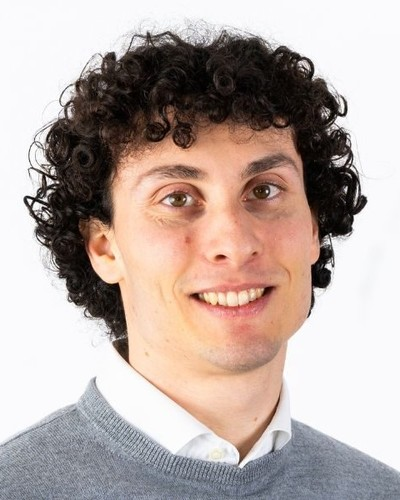
\includegraphics[width=1in,height=1.25in,clip,keepaspectratio]{figures/bio/brancato.jpg}}]{Lorenzo Brancato}
received the Ph.D. degree in mechanical engineering from Politecnico di Milano, Milan, Italy, in 2026. He is currently a Postdoctoral Researcher with the Department of Mechanical Engineering, Politecnico di Milano, where he works on the BATTAGE and EXTESA projects. His research focuses on prognostics and health management of critical systems, combining high-fidelity physics-based models with data-driven methods. He develops model-based state estimators and physics-informed operator learning for lithium-ion batteries, targeting state-of-charge estimation and the early detection and localization of internal short circuits. He also works on unsupervised anomaly detection in satellite telemetry and on digital twins for health monitoring of aerospace systems.
\end{IEEEbiography}
\vspace{-6mm}
\begin{IEEEbiography}[{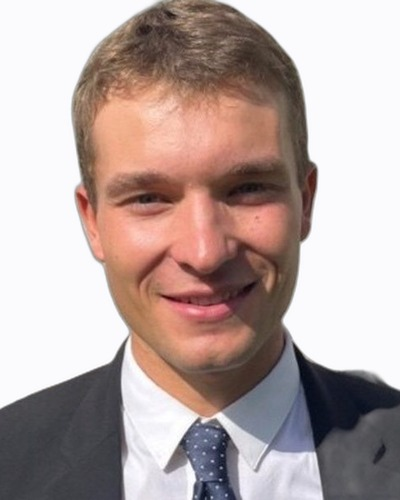
\includegraphics[width=1in,height=1.25in,clip,keepaspectratio]{figures/bio/harej.jpg}}]{Alexander Gabriel Harej}
is with the Department of Mechanical Engineering, Politecnico di Milano, Milan, Italy. His research focuses on health monitoring of lithium-ion batteries, combining physics-based electrochemical models with data-driven methods. Starting from a surrogate of the single particle model embedded in a Kalman filter for real-time state-of-charge estimation, his work now extends to state-of-health tracking and remaining useful life prediction, with a particular interest in operator networks.
\end{IEEEbiography}
\vspace{-6mm}
\begin{IEEEbiography}[{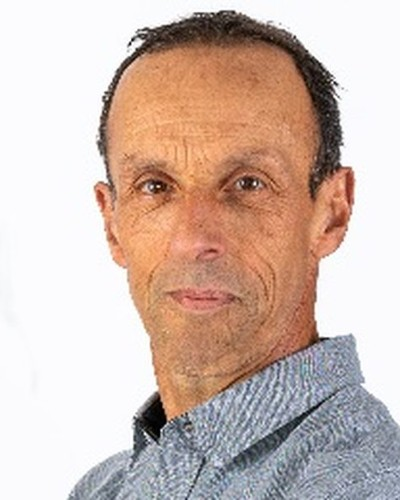
\includegraphics[width=1in,height=1.25in,clip,keepaspectratio]{figures/bio/giglio.jpg}}]{Marco Giglio}
graduated (cum laude) from Politecnico di Milano, Milan, Italy, in 1988. He is a Full Professor of Machine Design with the Department of Mechanical Engineering, Politecnico di Milano, and the Scientific Coordinator and Team Leader of SIGMA Lab. His research addresses the structural integrity of mechanical and aeronautical components and systems, from structural health monitoring and prognosis of helicopters and UAVs to ballistic impact, fatigue and crack growth. He has coordinated five European Defence Agency (EDA) projects, from HECTOR in 2009 to BATTAGE, started in 2025, and has been a Governmental Expert in the EDA CapTech Aerial Systems and Materials \& Structures since 2018. He has headed the department's Machine Design and Vehicles Section since 2013, and was Deputy Head of the department in 2018--2019. He has published more than 260 papers indexed in Scopus and was included in the October 2023 World Top 2\% Scientists ranking.
\end{IEEEbiography}
\vspace{-6mm}
\begin{IEEEbiography}[{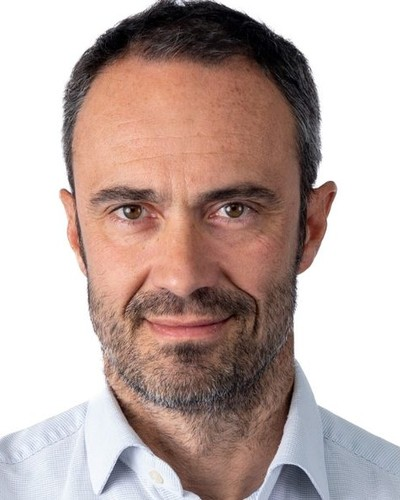
\includegraphics[width=1in,height=1.25in,clip,keepaspectratio]{figures/bio/cadini.jpg}}]{Francesco Cadini}
received the M.Sc. degree in aerospace engineering from the University of California, Los Angeles, CA, USA, in 2003, and the Ph.D. degree in radiation science and engineering from Politecnico di Milano, Milan, Italy, in 2006. He is an Associate Professor of Machine Design with the Department of Mechanical Engineering, Politecnico di Milano, where he is a core member of the SIGMA Lab research group. His research focuses on AI/ML-based methods for the integrity of complex engineering systems (structural health monitoring, prognostics and health management, digital twins, hybrid physics/data-driven modelling, explainable AI and uncertainty quantification), with applications to aerospace and space platforms, UAVs, lithium-ion and structural batteries, and defence systems. He is currently Scientific Coordinator or unit coordinator of several European (EDA, EDF) and national (ASI, MoD) research projects, including BATTAGE, COMMANDS, FMBTech, SYBIL, DIGES and EXTESA.
\end{IEEEbiography}

\end{document}
